\documentclass[11pt,a4paper,ngerman]{report}
% sostituire con report/book per il formato elettronico

\usepackage[nottoc,notlof,notbib,notindex]{tocbibind} % include l'elenco delle figure e la bibliografia nell'indice.
\usepackage{url}
\usepackage{pdfpages}
\usepackage{tocloft}
\usepackage{appendix}
\usepackage{tabularx, caption, boldline}
\usepackage{array}
%\usepackage{multirow}
\usepackage[ngerman, english]{babel}
\usepackage{ucs} %unicode sistema gli accenti
\usepackage[utf8]{inputenc} %unicode sistema gli accenti utf8x
\usepackage{csquotes}
\usepackage[bottom]{footmisc} % posiziona le note in footer sempre in basso
\usepackage{fancyhdr}
\usepackage{graphicx}
\usepackage{color}
%\usepackage{subfigure} % per figure affiancate
\usepackage{subcaption}
\usepackage{supertabular} % used to break tables
\usepackage{float} % per far bene le figures
%\usepackage{indentfirst}
\usepackage[Lenny]{fncychap} % per cambiare i capitoli
\usepackage{longtable} % piazza le note nelle tabelle fuori dalla tabella e permette tabelle che spannano su più pagine
\usepackage{lastpage} % total page count
\usepackage[hyphens]{url}
%\usepackage{breakurl}
\usepackage{tikz}
\usepackage{verbatim}
\usepackage{amsmath}
\usepackage{amssymb}
\usepackage{comment}
\usepackage[colorlinks=true, pdfstartview=FitV, linkcolor=blue, citecolor=blue, urlcolor=blue,breaklinks=true]{hyperref}
\usepackage{listings}
\usepackage{xcolor}
\usepackage{booktabs}
\usepackage{wrapfig}

\usepackage[T1]{fontenc}
\usepackage{inconsolata}


\definecolor{pblue}{rgb}{0.13,0.13,1}
\definecolor{pgreen}{rgb}{0,0.5,0}
\definecolor{pred}{rgb}{0.9,0,0}
\definecolor{pgrey}{rgb}{0.46,0.45,0.48}


% colori e variabili
% color definitions
\definecolor{red}{rgb}{0.9,0.1,0.1}
\definecolor{blue}{rgb}{0.07,0.55,0.73}
\definecolor{purple}{rgb}{0.4,0.3,0.4}
\definecolor{deep}{rgb}{0.1,0.07,0.3}
\definecolor{white}{rgb}{0.9,0.8,0.86}
% per modificare il colore dei link andare su layout.tex
%layout legacy commands
\renewcommand{\sectionmark}[1]{\markright{\thesection.\ #1}}
\renewcommand{\chaptermark}[1]{\markboth{\thechapter.\ #1}{}}

%user defined commands

% defnisce una pagina bianca con stile plain (migliore delle pagine bianche inserite in automatico dal model book)
\newcommand{\blankpage}{
	\newpage
	% toglie la barra alta dalla pagina vuota
	\thispagestyle{plain}
	% forza una pagina vuota
	\mbox{}
	\newpage
}

%comando per inserire la premessa nel documento (fuori indice)
\newcommand{\premise}[1][]{
	\renewcommand{\theenumi}{#1\roman{enumi}}
	\renewcommand{\labelenumi}{(\theenumi)}
	\thispagestyle{plain}
}


%comandi creati per le convenzioni del documento:
\newcommand{\istage}{\textit{stage}}
\newcommand{\iStage}{\textit{Stage}}
\newcommand{\idfda}{\textit{D.F.D. Assessment System}}
\newcommand{\idfd}{\textit{D.F.D. Consulting}}
\newcommand{\iIT}{\textit{IT}}
\newcommand{\iICT}{\textit{ICT}}
\newcommand{\ibusiness}{\textit{business}}





% indice analitico (comandi con la 'i' scrivono e aggiungono, quelli con 'ii' aggiungono solo, quelli senza niente scrivono solo)
\newcommand{\iASI}{ASI\index{ASI}} %scrive C sharp

%tecnologie
\newcommand{\CSharp}{C♯} %scrive C sharp
\newcommand{\iCSharp}{C♯\index{C♯}} % scrive C sharp e aggiunge l'indice %\unichar{9839}
\newcommand{\idotNET}{.NET\index{.NET}} % scrive .NEt e aggiunge l'indice
\newcommand{\iiWPF}{\index{WPF}} % aggiunge solo l'indice a WPF
\newcommand{\iWPF}{WPF\index{WPF}} % scrive WPF e aggiunge l'indice
\newcommand{\iiWF}{\index{WinForms}}
\newcommand{\iAW}{ANTLRWorks\index{ANTLRWorks}}
\newcommand{\iA}{ANTLR\index{ANTLR}}
\newcommand{\iU}{Unicode\index{Unicode}}
\newcommand{\iPSharp}{\texttt{PdfSharp}\index{PdfSharp@\texttt{PdfSharp}}}
\newcommand{\iTSharp}{\texttt{iTextSharp}\index{iTextSharp@\texttt{iTextSharp}}}

%grammatica
\newcommand{\iiCFG}{\index{CFG (context-free grammar)}}

%programmi
\newcommand{\iVS}{Visual Studio\index{Visual Studio}}
\newcommand{\iVSS}{Visual SourceSafe\index{Visual SourceSafe}}
\newcommand{\iSS}{SQL Server\index{SQL Server}}

% ciclo attivo e passivo
\newcommand{\iCA}{ciclo attivo\index{ciclo!attivo}} % scrive ciclo attivo e aggiunge l'indice
\newcommand{\iCP}{ciclo passivo\index{ciclo!passivo}} % scrive ciclo passivo e aggiunge l'indice
\newcommand{\iiCA}{\index{ciclo!attivo}} % aggiunge l'indice
\newcommand{\iiCP}{\index{ciclo!passivo}} % aggiunge l'indice
\newcommand{\iDCA}{ciclo attivo\index{documento!ciclo attivo}} % scrive ciclo attivo agigunge l'indice al ciclo attivo del documento
\newcommand{\iDCP}{ciclo passivo\index{documento!ciclo passivo}} % scrive ciclo passivo aggiunge l'indice al ciclo passivo del documento
\newcommand{\iiDCA}{\index{documento!ciclo attivo}} % aggiunge l'indice al ciclo attivo del documento
\newcommand{\iiDCP}{\index{documento!ciclo passivo}} % aggiunge l'indice al ciclo passivo del documento
\newcommand{\iGCA}{ciclo attivo\index{gestione!ciclo attivo}} % scrive ciclo attivo e aggiunge l'indice a gestione
\newcommand{\iGCP}{ciclo passivo\index{gestione!ciclo passivo}} % scrive ciclo passivo e aggiunge l'indice a gestione
\newcommand{\iiGCP}{\index{gestione!ciclo passivo}} % aggiunge l'indice a gestione

%componenti
\newcommand{\icMM}{\texttt{MapManager}\index{MapManager@\texttt{MapManager}}}
\newcommand{\iicMM}{\index{MapManager@\texttt{MapManager}}}
\newcommand{\icMF}{\texttt{MapFinder}\index{MapFinder@\texttt{MapFinder}}}
\newcommand{\iicMF}{\index{MapFinder@\texttt{MapFinder}}}
\newcommand{\icPA}{\texttt{PdfAnalyzer}\index{PdfAnalyzer (componente)@\texttt{PdfAnalyzer} (componente)}}

%package e classi
\newcommand{\iPFE}{\texttt{Plain.File.Extraction}\index{Plain.File.Extraction@\texttt{Plain.File.Extraction}}}
\newcommand{\iiPFE}{\index{Plain.File.Extraction@\texttt{Plain.File.Extraction}}}
\newcommand{\iPA}{\texttt{PdfAnalyzer}\index{Plain.File.Extraction@\texttt{Plain.File.Extraction}!PdfAnalyzer (classe)@\texttt{PdfAnalyzer} (classe)}}
\newcommand{\iPP}{\texttt{PdfPage}\index{Plain.File.Extraction@\texttt{Plain.File.Extraction}!PdfPage@\texttt{PdfPage}}}
\newcommand{\iPPar}{\texttt{PdfTextStreamParser}\index{Plain.File.Extraction@\texttt{Plain.File.Extraction}!PdfTextStreamParser@\texttt{PdfTextStreamParser}}}
\newcommand{\iPLex}{\texttt{PdfTextStreamLexer}\index{Plain.File.Extraction@\texttt{Plain.File.Extraction}!PdfTextStreamLexer@\texttt{PdfTextStreamLexer}}}
\newcommand{\iPF}{\texttt{PdfFont}\index{Plain.File.Extraction@\texttt{Plain.File.Extraction}!PdfFont@\texttt{PdfFont}}}
\newcommand{\iPT}{\texttt{PdfText}\index{Plain.File.Extraction@\texttt{Plain.File.Extraction}!PdfText@\texttt{PdfText}}}
\newcommand{\iPC}{\texttt{PdfChar}\index{Plain.File.Extraction@\texttt{Plain.File.Extraction}!PdfChar@\texttt{PdfChar}}}

%parti di un PDF
\newcommand{\iH}{\texttt{Header}\index{PDF!Header@\texttt{Header}}}
\newcommand{\iFT}{\texttt{File Trailer}\index{PDF!File Trailer@\texttt{File Trailer}}}
\newcommand{\iCRTable}{\texttt{Cross Reference Table}\index{PDF!Cross Reference Table@\texttt{Cross Reference Table}}}
\newcommand{\iB}{\texttt{Body}\index{PDF!Body@\texttt{Body}}}

% stream
\newcommand{\iS}{stream\index{stream}}
\newcommand{\iiS}{\index{stream}}
\newcommand{\iCS}{stream\index{content stream}}
\newcommand{\iiCS}{\index{content stream}}

%fasi dello stage
\newcommand{\iifS}{\index{studio del dominio!fase di}}
\newcommand{\iifA}{\index{analisi!fase di}}
\newcommand{\iifP}{\index{progettazione!fase di}}
\newcommand{\iifC}{\index{codifica!fase di}}
\newcommand{\iifV}{\index{verifica e validazione!fase di}}
\newcommand{\iifD}{\index{documentazione!fase di}}

%attività dello stage
\newcommand{\iiaS}{\index{studio del dominio!attività di}}
\newcommand{\iiaA}{\index{analisi!attività di}}
\newcommand{\iiaP}{\index{progettazione!attività di}}
\newcommand{\iiaC}{\index{codifica!attività di}}
\newcommand{\iiaV}{\index{verifica e validazione!attività di}}
\newcommand{\iiaD}{\index{documentazione!attività di}}

%matrici
\newcommand{\Tm}{$T_{m}$}
\newcommand{\Tlm}{$T_{lm}$}

%peratori
\newcommand{\Tc}{\texttt{Tc}\index{operatore!di stato}}
\newcommand{\Tw}{\texttt{Tw}\index{operatore!di stato}}
\newcommand{\Tz}{\texttt{Tz}\index{operatore!di stato}}
\newcommand{\TL}{\texttt{TL}\index{operatore!di stato}}
\newcommand{\Tf}{\texttt{Tf}\index{operatore!di stato}}
\newcommand{\Tr}{\texttt{Tr}\index{operatore!di stato}}
\newcommand{\Ts}{\texttt{Ts}\index{operatore!di stato}}

\newcommand{\Td}{\texttt{Td}\index{operatore!di posizionamento}}
\newcommand{\Tmm}{\texttt{Tm}\index{operatore!di posizionamento}}
\newcommand{\Tstar}{\texttt{T*}\index{operatore!di posizionamento}}

\newcommand{\Tj}{\texttt{Tj}\index{operatore!di stampa}}
\newcommand{\Tquote}{\texttt{'}\index{operatore!di stampa}}
\newcommand{\Tdblquote}{\texttt{\textquotedbl}\index{operatore!di stampa}}
\newcommand{\TJ}{\texttt{TJ}\index{operatore!di stampa}}










\graphicspath{{./pics/}} % cartella di salvataggio immagini

\pagestyle{fancy}

\lhead{\nouppercase{\rightmark}}
\rhead{\nouppercase{\leftmark}}

\fancypagestyle{plain}{
	\lhead{}
	\chead{}
	\rhead{}
	\lfoot{}
	\cfoot{\thepage}
	\rfoot{}
	\renewcommand{\headrulewidth}{0.0pt}% this command should not be add to variables.tex
	\renewcommand{\footrulewidth}{0.1pt}% this command should not be add to variables.tex
}

\fancypagestyle{blank}{
	\lhead{}
	\chead{}
	\rhead{\nouppercase{\rightmark}}
	\lfoot{}
	\cfoot{\thepage}
	\rfoot{}
	\renewcommand{\headrulewidth}{0.1pt}% this command should not be add to variables.tex
	\renewcommand{\footrulewidth}{0.1pt}% this command should not be add to variables.tex
}



% parte per il report
 %	\lhead{}
% 	\chead{}
% 	\rhead{\nouppercase{\rightmark}}
% 	\lfoot{}
% 	\cfoot{\thepage}
% 	\rfoot{}
% 	\renewcommand{\headrulewidth}{0.1pt}% this command should not be add to variables.tex
% 	\renewcommand{\footrulewidth}{0.1pt}% this command should not be add to variables.tex
 
 %\hypersetup{
 %	colorlinks=true,% false: boxed links; true: colored links
% 	linkcolor=blue,% color of internal links
% 	urlcolor=blue,% color of external links
% 	anchorcolor = blue,
% 	citecolor = blue
 %}
%parte per il report



% parte per il book
\fancyhead{}
%\fancyhead[EL]{\nouppercase{\leftmark}}
\fancyhead[OR]{\nouppercase{\rightmark}}
%\fancyfoot[EC,OC]{\thepage}

	\renewcommand{\headrulewidth}{0.1pt}% this command should not be add to variables.tex
	\renewcommand{\footrulewidth}{0.1pt}% this command should not be add to variables.tex
\hypersetup{
	colorlinks=true,% false: boxed links; true: colored links
	linkcolor=black,% color of internal links
	urlcolor=black,% color of external links
	anchorcolor = black,
	citecolor = black
}
%parte per il book
\newcommand{\changelocaltocdepth}[1]{%
	\addtocontents{toc}{\protect\setcounter{tocdepth}{#1}}%
	\setcounter{tocdepth}{#1}%
}

\setlength{\parindent}{0pt}

% indice analitico
\usepackage{makeidx}
\makeindex 

\let\textquotedbl=" % use to print also " in the code


\bibliographystyle{plain}%bibliografia stile inglese

\pagenumbering{Roman}
% fine layout

\newcommand{\figuresource}[1]{\small \par Quelle: #1}

\colorlet{punct}{red!60!black}
\definecolor{background}{HTML}{EEEEEE}
\definecolor{delim}{RGB}{20,105,176}
\colorlet{numb}{magenta!60!black}

\definecolor{pblue}{rgb}{0.13,0.13,1}
\definecolor{pgreen}{rgb}{0,0.5,0}
\definecolor{pred}{rgb}{0.9,0,0}
\definecolor{pgrey}{rgb}{0.46,0.45,0.48}

\lstset{language=Java,
  basicstyle=\footnotesize=7\ttfamily,
  morekeywords={@NotNull},
  numbers=left,
  stepnumber=1,
  showspaces=false,
  frame=lines,
  showtabs=false,
  breaklines=true,
  showstringspaces=false,
  breakatwhitespace=true,
  commentstyle=\color{pgreen},
  backgroundcolor=\color{background},
  keywordstyle=\color{pblue},
  stringstyle=\color{pred},
  moredelim=[il][\textcolor{pgrey}]{$$},
  moredelim=[is][\textcolor{pgrey}]{\%\%}{\%\%}
}

\lstdefinelanguage{json}{
	basicstyle=\normalfont\ttfamily,
	numbers=left,
	numberstyle=\scriptsize,
	stepnumber=1,
	showstringspaces=false,
	breaklines=true,
	frame=lines,
	backgroundcolor=\color{background},
	literate=
	{0}{{{\color{numb}0}}}{1}
	{1}{{{\color{numb}1}}}{1}
	{2}{{{\color{numb}2}}}{1}
	{3}{{{\color{numb}3}}}{1}
	{4}{{{\color{numb}4}}}{1}
	{5}{{{\color{numb}5}}}{1}
	{6}{{{\color{numb}6}}}{1}
	{7}{{{\color{numb}7}}}{1}
	{8}{{{\color{numb}8}}}{1}
	{9}{{{\color{numb}9}}}{1}
	{:}{{{\color{punct}{:}}}}{1}
	{,}{{{\color{punct}{,}}}}{1}
	{\{}{{{\color{delim}{\{}}}}{1}
	{\}}{{{\color{delim}{\}}}}}{1}
	{[}{{{\color{delim}{[}}}}{1}
	{]}{{{\color{delim}{]}}}}{1},
}

\lstdefinelanguage{SQL}{
	basicstyle=\normalfont\ttfamily,
	numbers=left,
	numberstyle=\scriptsize,
	stepnumber=1,
	numbersep=8pt,
	showstringspaces=false,
	breaklines=true,
	frame=lines,
	backgroundcolor=\color{background},
	literate=
	{0}{{{\color{numb}0}}}{1}
	{1}{{{\color{numb}1}}}{1}
	{2}{{{\color{numb}2}}}{1}
	{3}{{{\color{numb}3}}}{1}
	{4}{{{\color{numb}4}}}{1}
	{5}{{{\color{numb}5}}}{1}
	{6}{{{\color{numb}6}}}{1}
	{7}{{{\color{numb}7}}}{1}
	{8}{{{\color{numb}8}}}{1}
	{9}{{{\color{numb}9}}}{1}
	{:}{{{\color{punct}{:}}}}{1}
	{,}{{{\color{punct}{,}}}}{1}
	{\{}{{{\color{delim}{\{}}}}{1}
	{\}}{{{\color{delim}{\}}}}}{1}
	{[}{{{\color{delim}{[}}}}{1}
	{]}{{{\color{delim}{]}}}}{1},
}

\newcommand{\TODO}[1]{\marginpar{\color{red}\emph{\small{{\bf TODO: } #1}}}}
% layout
\begin{document}
%\hyphenation{
Plugin-Arch-it-ekt-ur
}


%word division

\selectlanguage{ngerman}

% Frontespizio
\begin{titlepage}
\begin{center}
	\vspace{6em}
	{\Large \textsc{Projektbericht}}\\
	\vspace{5em}
	{\huge \textsc{Hamaube}}\\
	\vspace{4em}
	{\Large \textsc{Kai Martinen, Fabian Kohler, Merlin Koglin, Arkadij Daschkewitsch, Rasmus Warrelmann, David Zschocke }}\\
	\vspace{3em}
	{\Large \textsc{\today}}\\
	\vspace{3em}
	
\includegraphics[scale=0.4]{uni-logo.jpg}\\
	\vspace{3em}
	{\Large \textsc{Universität Hamburg}}\\
	\vspace{1em}
	{\Large \textsc{Department of Computer Science}}\\
	\vspace{1em}
	{\Large \textsc{Chair of Distributed Systems and Information Systems}}\\
	\vspace{2em}
	{\Large \textsc{Betreut durch Steffen Friedrich}}\\
	
\end{center}
\end{titlepage}%for the cover title

%If want to write a dedication, modify the following.
%\dedication{Zitat, kluger Spruch oder Widmung}

\newpage
% brauchen wir nicht auf englsich. das liest eh nur steffen :D
%\chapter*{Abstract}
%\addcontentsline{toc}{chapter}{Abstract}
%Abstract in English

\chapter*{Kurzfassung}
\addcontentsline{toc}{chapter}{Kurzfassung} 
Diese Arbeit behandelt die Modularisierung und die Erweiterung des Petrinetz Simulators \textit{Renew} auf eine Mikroservice-Architektur.
\textit{Renew} wurde für die Modellierung von komplexen Systemen mit Hilfe der Petri Netze entwickelt. Da die Software viel Fachwissen voraussetze und sensibel auf Änderungen ungeübter Entwickler reagierte, entstand eine Plugin-Architektur, die \textit{Renew} mit Funktionalität anreichern lies ohne ihre innere Struktur zu verletzen. Diese Architektur ermöglichte die Entwicklung einer Großzahl an Plugins von Mitarbeitern aus verschiedenen Forschungsbereichen.
Dementsprechend blieb die Plugin-Architektur von \textit{Renew} in den letzten sechzehn Jahren unverändert.     
\bigbreak
Obwohl die Plugin-Architektur sich damit langfristig bewährt hat, ist sie nicht für die modernen Herausforderungen gewappnet. Da die moderne Rechenleistung sich in der parallelen und verteilten Datenverarbeitung befindet, kann \textit{Renew} in jetzigem Zustand sich diese nicht zunutze machen. 
Ziel dieser Arbeit ist die Vorbereitung und Umstrukturierung von \textit{Renew} für die Mikroservice-Architektur, um ihre interne Struktur verteilt ausführen zu können.
\bigbreak
Hier kommt der Stand der Dinge nachdem ich in der bib gesucht habe und wahrscheinlich nix finde.
Da hab ich was \hyperlink{https://kataloge.uni-hamburg.de/DB=1/SET=1/TTL=1/SHW?FRST=10}{\underline{ inf bib}} 
Noch was \hyperlink{https://kataloge.uni-hamburg.de/DB=1/SET=2/TTL=10/SHW?FRST=6}{\underline{kummer 2002 defenition Referenznetze}}
\bigbreak
Im ersten Abschnitt diese Arbeit wird die Code-Basis umstrukturiert und gestaltet \textit{Renew} modular. Folgerichtig wird \textit{Renew} auf die Korrektheit überprüft und nicht mehr unterstützten Legacy Architektur Entscheidungen überarbeitet. 
Im zweiten Abschnitt wird ein Teil von \textit{Renew} distributiv aufgesetzt.
Zum Schluss folgt eine Bewertung und Aussichten für die Weiterentwicklung von \textit{Renew}.




% Old Abstract
%\newpage
%\blankpage
%\premise{
%\noindent{\textbf{\begin{huge}Abstract\end{huge}}}\\
%\\
%Abstract 
%}
\linespread{1.25}\selectfont

% Wenn ihr Pakete braucht dann bindet die bitte in layout.tex ein und scheibt eine mail rum damit alle anderen merge konflikte vermeiden können.
\changelocaltocdepth{1}
\tableofcontents % indice dei contenuti
 %lista delle figure
\setcounter{lofdepth}{4}
 \listoffigures
%\listoftables
\blankpage
%\blankpage
\chapter{Einleitung}
\pagenumbering{arabic}

\section{Petrinetze} 
Das Konzept der Petrinetze wurde in der Arbeit von \textit{Carl Petri} beschrieben. 
Dieses besteht aus Stellen, Marken, Kanten und Transitionen, das nebenläufige und kommunizierende Prozesse darstellen kann.
Der ursprüngliche S/T-Netz Formalismus wurde mit der Zeit durch gefärbten Marken erweitert, mit dem Ziel äquivalente Strukturen zusammenzufassen und die darin befindlichen Marken zu typisieren.
Da die Struktur des Netzes immer noch stark zusammenhängend ist, bleibt die Organisation des Netzes schwer verständlich für das menschliche Auge. \newline 
Demzufolge sollte des Netzes auf logisch zusammenhänge Komponente aufgeteilt werden und trotzdem als ein Ganzes gelten.
Diese Anforderung wird von den synchronen Kanälen umgesetzt, indem die Netzkomponenten anstelle der Kanten mit synchronen Kanälen verbunden werden und zwingen die mit einander verbunden Transitionen synchron zu schalten.
Hiermit ist eine Trennung des Netzes nach ihrer Funktionalität erreicht, die qualitativ anspruchsvolle Modelle komplexer und verteilter Systeme entwerfen lässt.\bigbreak
Obwohl das erweiterte Petrinetz anspruchsvolle Modellierungswerkzeug bietet, bleibt das gesamte Netzwerk statisch.
Demzufolge wurde der nächste Evolutionsschritt in der Entwicklung der Petrinetze mit den Referenznetz Formalismus gemacht. 
Dieser erlaubt dynamisch und bei Bedarf Netzinstanzen zu erstellen und diese als Marken in einem anderen Netz zu bewegen. 
Somit kann es mehrerer Instanzen eines Netzes geben, die mit unterschiedlicher Belegung im Petrinetz existieren. 

\section{Renew} 
Renew ist ein Petrinetz Simulator, der die oben genannten Petrinetz Formalismen unterstützt. Dieser ist in Java geschrieben und bietet eine Oberfläche zum Zeichnen und einen Simulator zum Ausführen der Netze. \newline 
Da die empfindliche monolithische Architektur von Olaf Kummer viel Fachwissen voraussetzte, wurde diese zu einem Plugin Verband von Jörn Schumacher zu Gunsten der Robustheit und Erweiterung umstrukturiert. Nun kann Renew über die Plugin Schnittstellen erweitert werden, ohne die existierende Logik zu beeinflussen. \bigbreak
Mit seiner Umsetzung delegierte Jörn Schumacher die Ausführung von Logik an Plugins und erstellte eine zentrale Instanz, die den Lebenszyklus bekannter Plugins verwaltet und koordiniert. Die zentrale Instanz nennt sich Plugin-Manager und kann das Verhalten von Renew mit Hilfe der Plugins modifizieren.
Der Plugin-Manager baut auf zwei primären Namespaces auf. Zum einen braucht dieser zusätzliche Bibliotheken zum verwalten seiner Umgebung und zum anderen braucht er Plugins, die Funktionalität mit sich bringen. 
\bigbreak 

\section{Gegenstand}
Mit der Plugin Architektur hat Renew ihren Lebenszyklus weit überschritten, denn der Plugin-Manager und die Kernfunktionalität blieb lang unverändert. An manchen Stellen datiert die Code Basis aus dem Jahr 2002 (JDK 1.4). 
Somit entsprechen die erstmaligen Gestaltungsmöglichkeiten, Architekturentscheidungen und ihre Umsetzung, nicht mehr den aktuellen Stand der Technik (JDK 11). Vor allem durch die Einführung des Modulsystem von Java 9, mit dem der JDK sowie der darauf aufbauenden Code modularisiert wird. 
Im Zuge dessen ist das Portieren der Applikation nicht mängelfrei. Es ist unklar wie sich die benutzerdefinierten Namensräume und die so gut wie unberührten Kern-Plugins auf die neuen Modulstruktur übertragen lassen. Zumal die Suche nach zusätzlichen Plugin-Code eine zentrale Funktion in System vertretet.\bigbreak
Indem die Applikation neu strukturiert wird, sind zusätzliche Mängel zu erwarten, denn das Vernachlässigen der Gesamtarchitektur und die Konzentration nur auf das eigne Plugin führt zu Code-Duplizierung und Problemen in der Verständlichkeit der Plugin-Abhängigkeiten.\newline
Beifolgend stellt sich die Frage: Wie Portierbar ist Renew und was muss getan werden damit der Umstieg auf Java 11 gelingt. \bigbreak

\section{Ziel} 
Das Ziel dieser Arbeit ist die Anpassung von Renew an die neuen Anforderungen der Java Laufzeitumgebung sowie das Ausarbeiten einer möglichen Architektur für die verteilte Ausführung. Dementsprechend soll Renew einen einfachen Einstig in die existierende Kernlogik geben, sowie die Entwickler-Fähigkeiten in der Forschung verteilter Systeme vorantreiben, indem  selbst erstellte Simulation verteilt ausgeführt werden dürfen.

%- Ziel : Mikroservice
%- Wieso Mikroservices? 
%- Bis zum Ziel müssen die Plugins modularisiert werden
%- Die Plugins müssen sinnvoll gesplittet und die Berechnungsaufgabe aufgeteilt werden.
%- Es muss eine Kommunikationsinfrastruktur aufgestellt werden
%- Es müssen Umsetzungen von verteilten System evaluiert werden. 
\section{Umsetzung}
% Umsetzung
% Anforderungen
% Vergleich Umsätzung ähnlicher Anforderungen
1. Es entsteht ein Prototyp 
	- Dieser restrukturiert ein Teil von Renew modular.
	- Somit wird die Code Base, sowie Design-Entscheidungen modernisiert und auf die Java 11 Version angepasst. Dabei soll der Schwerpunkt beim Plugin-Manager liegen, der die zentrale Aufgabe der Plugin-Verwaltung trägt.    
	- Um die Plugins ausführen zu können, sollten die Plugins mit Hilfe des Gradle Build Tools compiliert und ausführbar verpackt werden. 
	-  Als nächstes sollten die Plugins fähig sein Verteilt und Kooperative arbeiten zu können. Dafür wird eine Architektur benötigt, die den modularen Prototypen erweitert. Somit einsteht eine Mikroservices-Architektur, die von einander unabhängig Einheiten ein globales Ziele verfolgen lässt. 
2. Da viele Modernen Applikationen ihre Code Base aufteilen und verteilt ausführen lassen, werde ich mehrere Umsetzungen untersuchen und die Vor- und Nachteile untersuchen. Die Rezension wird die Entscheidung für die Umsetzung der Verteilten Architektur beeinflussen.

% was muss getan werden um die Ziele zu erreichen, 
% was muss ich lesen lernen und analysieren,
% was kommt dabei raus 
- Java 9 und Module erste schritte zu Mikroservice und verteilten Anwendung  
- Java EE  EE Kontainer
- Swagger 
- Kafka
- Web Interface 
\section{Aufbau der Arbeit}
% Aufbau der Arbeit 
Hier kommt der Aufbau 


\chapter{Architektur}

\section{Einführung}
Ziel des Projekt ist es einen Twitter-Klon zu entwickeln. Als Mikroblogging-Dienst ist die zentrale Funktionalität:
\begin{itemize}
  \item Senden von Tweets
  \item Finden von Tweets (Anzeigen der Tweets in der eigenen Timeline, Suchen nach Schlüsselwörten/Hashtags)
\end{itemize}
Zusätzlich ist selbstverständlich eine Benutzerverwaltung nötig. Ebenso interessant sind Analytics-Funktionalitäten.

In diesem Projekt liegt der Fokus auf der Entwicklung  einer Architektur, die besondere Nicht-Funktionale Anforderungen
erfüllt. Diese ergeben sich aus den Anforderungen an das reale Twitter:
\begin{itemize}
  \item Skalierbarkeit
  \item Erweiterbarkeit um zusätzliche Funktionalität.
\end{itemize}

Geprägt ist Twitter durch enorme Datengeschwindigkeit (Velocity in Gartners Vs). Jede Sekunde werden im
Durchschnitt 6000 Tweets weltweit abgesetzt. Diese Zahlen varieren zudem
stark: Der Rekord liegt bei 140.000 Tweets pro Sekunde\footnote{\url{https://www.brandwatch.com/de/blog/twitter-statistiken/}
\url{http://www.gegen-den-strom.org/twitter/}}.. Zudem werden viele Features von Twitter nach und nach eingeführt,
ohne das Twitter in Wartungspausen geht (gehen musste).

Diesen Herausforderungen sind herkömmliche Webarchitekturen nicht gewachsen. Dieses Projekt entwickelt einen Twitter-Clon
mit den Technologien und einer Architektur, die diesen Anforderen im Prinzip gewachsen ist.

\section{Entwicklung der neuen Architektur}
Ausgangspunkt der Entwicklung der neuen Architektur ist eine einfache Client-Server-Architektur. Es gibt in ihr einen Server
mit viel Rechnenleistung sowie viele Clients. Die Clients verbinden sich mit dem Server, der sie parallel bedient. Die Parallellisierung
erfolgt also auf Thread-/Prozessebene.

Der nächste Schritt ist es, die Datenhaltung in eine Datenbank auszulagern. Es gibt jetzt drei Komponenten: die Clients,
der Webserver und der Datenbankserver. Wenn die Leistung des Serversystems nicht ausreicht gibt es unterschiedliche Möglichkeiten
für mehr Leistung zu sorgen:
\begin{itemize}
  \item Die einzelnen Server mit mehr Leistung auszustatten
  \item Mehr Webserver einzuführen
\end{itemize}
Möglichkeit 1 würde ein Aufrüsten der Server mit schnelleren Prozessoren, mehr Arbeitsspeicher, schnelleren Festplatten etc.
bedeuten. Möglichkeit 2 ist schon etwas komplizierter. Zwar werden die Daten zentral vom Datenbankserver gehalten,
trotzdem können nicht einfach mehr Webserver eingeführt werden. Die Clients müssen noch auf die Webserver verteilt werden.

Diese Aufgabe kann wieder auf zwei Arten erfolgen: Im Netzwerkprotokoll (z.B: über Anycast) oder durch eine zusätzliche
Komponente im Server, nämlich dem Load-Balancer. An ihn kommen alle Anfragen an die Webserver und der Loadbalancer
entscheidet mit mehr oder weniger komplexe Techniken welcher Webserver genutzt werden soll und leitet
den anfragenden Client an diesen Webserver weiter. Dabei achtet diese Komponete z.B. darauf, dass bereits stark
ausgelastete Webserver keine neuen Clients mehr zugewiesen bekommen, sondern nur Webserver mit aktuell
niedriger Auslastung.

Die Parallelisierung erfolgt in dieser Architektur bereits auf vielen Ebenen: Im Loadbalancer, in den Webservern und in der
Datenbank. Die Datenbank führt dafür ausgefeilte Mechansimen zur Verwaltung der parallelen Anfragen und zur
Datenkonsistenz aus.

Diese Architektur wird häufig mit dem LAMP Softwarestack implementiert: Linux als Betriebssystem der Server,
Apache als Webserver, MySQL als Datenbank und PHP als Serverprogrammiersprache.

So weit eine erste Einführung in die Verteilung von Webanwendungen mit herkömmlichen Architekturen.
Nun wollen wir die Art der Verteilung analysieren um darzustellen, weshalb eine andere Architektur für noch
mehr Verteilung nötig ist.

\subsection{Analyse der Verteilung}
Es kommen zwei Techniken der Verteilung zu Einsatz
\begin{itemize}
  \item Erhöhung der Rechenleistung der einzelnen Komponenten
  \item Loadbalancing
\end{itemize}

Die erste Technik wird auch Scale-Up genannt. Durch potentere Hardware kann ein Leistungszuwachs erzielt werden.
Allerdings - und das ist ein zentrales Problem, dass unsere neue Architektur lösen wird - sind dieser Möglichkeit
vergleichsweise enge Grenzen gesetzt. Der Prozessorgeschwindigkeit sind durch die Eigenschaften des verwendeten
Silizium und der Wärmeentwicklung enge Grenzen gesetzt. Über 5 GHz gehen die Taktraten nicht mehr hinaus.
Damit ist bereits bei einem Faktor von ca. 2,5 der Geschwindigkeitserhöhung hier ein Ende gesetzt. Von 2 GHz
geht es bis maximal 5 GHz hoch (und selbst 5 GHz erreichen die wenigsten Prozessoren). Ein Leistungszuwachs
kann jetzt nur noch durch mehr Prozessorkerne und mehr Prozessoren erreicht werden. Durch mehrere Sockel
in den Server (leicht bis zu 4 Stück) und mehr Kernen in den Prozessoren (leicht bis zu 20 Stück) lässt sich hier
bei sehr guter Parallelisierbarkeit der Anwendung\footnote{Amdahl‘s Law zeigt, dass sich durch mehr
Hardware die Geschwindigkeit nicht linear erhöht} theoretisch eine Erhöhung um das 80-fache erreichen.

Hier ist nun die Grenze für das Scale-Up erreicht. Herkömmliche Server lassen sich nun kaum mehr beschleunigen.
Sobald also eine Komponente in unserer Architektur mehr Leistung benötigt weil mehr Client-Anfragen kommen,
als sie bearbeiten kann, müssen wir etwas in der Architektur ändern. Die Ausnahme sind hier die Webserver.
In unserer Architektur können wir bereits mehr Webserver hinzufügen und die Last auf mehr Rechner verteilen,
anstatt auf schnellere Rechner. Das ist ein Grundgedanke unserer neuen Architektur. Im Gegensatz zum Scale-Up
wird dieser Ansatz Scale-Out genannt.

Die Komponente, die dementsprechend als erstes in unserer Architektur geändert werden muss, ist die Datenbank.
Damit beschäftigen wir uns im nächsten Abschnitt.

\subsection{Die Verteilung der Datenbank}
Wir müssen also unsere Datenbank beschleunigen. Wir nehmen an, dass wir kein Scale-Up mehr durchführen können oder
wollen.

Eine Möglichkeit wäre noch die Nutzung von sehr spezialisierter Datenbankhardware. Diese hat sehr große Investitionskosten
und legt einen auf eine spezielle Datenbanksoftware fest. Wir möchten diese deshalb nicht betrachten.

Ein erster Ansatz wäre es, das Load-Balancing der Webserver zu wiederholen. Mehr Datenbankserver und eine Komponente,
die die Anfragen an einen Datenbankserver mit genug verfügbarer Kapazität weiterleitet. Allerdings geht das
nicht mehr so einfach wie bei den Webservern. Die Webserver waren untereinander unabhängig. Die Datenbank ist
das nicht. Man kann nicht einfach einen Datenbankserver nehmen und dort Daten ändern. Wird der Nutzer nun
bei seiner nächsten Anfrage an einen anderen Datenbankserver geleitet, sind die Änderungen dort nicht vorgenommen.
Das ist also keine Alternative.

Aber diesen Ansatz kann man noch verfeinern und schlussendlich gewinnbringend einsetzen.  Das Problem war,
dass die geänderten Daten nur auf einem Server verändert wurden und der User plötzlich auf einen anderen
Datenbankserver landete. Dann muss der Nutzer also immer auf dem gleichen Datenbankserver landen.
Eine einfache Möglichkeit der Verteilung wäre es also, die Nutzer fest auf die Datenbankserver zu verteilen.
Beispielsweise werden alle Nutzer mit Nachnamen, die mit A-K beginnen auf den ersten Datenbankserver zugewiesen,
die anderen auf den zweiten Datenbankserver. In Verwaltungseinrichtungen wird so etwas sogar physisch betrieben.
Wenn der Nutzer nun ein zweites Mal kommt, wird er wieder an den gleichen Datenbankserver weitergeleitet und
seine Daten sind dort aktuell. Diese Aufteilung muss dann aber in der Applikationslogik fest eingebaut werden.
Besser wäre es, wenn das automatisch passieren würde.

Der andere Ansatz wäre es nicht den Benutzer immer auf den gleichen Datenbankserver weiterzuleiten, sondern
die Datenbankserver alle aktuell zu halten. Dann wäre es wieder egal, welchen Datenbankserver er beim nächsten
Besuch nutzt. Allerdings sieht man sofort, dass dann sehr viel Netzwerkverkehr nötig wäre um die Daten auf allen
Server aktuell zu halten. Es ist also zweifelhaft, ob das so viel schneller wäre.

Das wiederum hängt vom Nutzungsprofil ab. Wenn Daten z.B. nur selten geändert werden, aber häufig gelesen,
dann ergibt das wieder Sinn. Der Overhead für das Aktuellhalten der Daten wäre dann sehr gering und
der Leseoperationen würden skalieren. 

\subsection{Ein erste Blick auf die neue Architektur}
Im vorigen Abschnitt haben wir gesehen, dass es nötig wird die Datenbank verteilt auszulegen. Die eine Möglichkeit war
die händische Aufteilung der Anfragen auf verschiedene, unabhängige Datenbankserver. Diese Möglichkeit ist aufwendig.
Eine andere Möglichkeit war das Spiegeln auf mehrere Datenbankserver. Das funktioniert nur dann, wenn die Leseoperationen
die Schreiboperationen weit übertreffen und die Schreiboperationen nur eine Last erzeugen, die ein einzelner Datenbankserver
bearbeiten kann.

Nun betrachten wir eine dritte Möglichkeit: die Verwendung verteilter Datenbanken. Damit werden Datenbankprogramme
bezeichnet, die für den Einsatz auf mehreren Servern gebaut wurden. Sie sind eine Spielart der so genannten NoSQL-Datenbanken.
Zur Skalierung verwenden sie den Scale-Out-Ansatz statt des Scale-Up-Ansatzes. D.h. sie sind so designed, dass man mehr
Leistungsfähigkeit durch das Einbinden weiterer Server erreichen kann. Diese Server bestehen aus herkömmlicher Serverhardware.
Es ist keine spezialisierte Hardware erforderlich. Die Koordinierung erfolgt über Netzwerkprotokolle. Damit wandert die
Skalierbarkeit in die Software. Die Realisierung wird weiter untem in einem gesonderten Kapitel beschrieben.

In der herkömmlichen Architektur wird nun die SQL-Datenbank durch eine verteilte Datenbank ersetzt. Jetzt lässt sich
die benötigte Leistung durch die Verteilung der Datenbank auf genügend Server erreichen. Diese Komponente ist
zusätzlich noch skalierbar, d.h. wenn mehr Leistung benötigt wird, können weitere Server hinzugefügt werden.

Das ist ein Prinzip unserer neuen Architektur: Nicht skalierbare Softwarekomponenten werden durch skalierbare
Softwarekomponenten ausgetauscht. Wir haben mit der Datenbank begonnen. Jetzt ist es Zeit die benötigten Komponenten
für unseren Twitter-Klon zu ermitteln. Im nächsten Schritt setzen wir für die Komponenten Software ein, die skalierbar ist.

\subsection{Benötigte Komponenten}
Unser Twitter-Klon soll die folgende Funktionalität haben:
\begin{itemize}
  \item Nutzerverwaltung: Benutzerkonto mit Login-Funktionalitöt
  \item Kernfunktionalität: Tweets senden und lesen
  \item Tweets entdecken: Tweets suchen und Empfehlungen bekommen
  \item Statistische Auswertungen der Tweets
\end{itemize}

Es gibt offensichtlich eine Frontend-Komponente. Das Backend besteht nun aus verschiedenen Komponenten. Eine Komponente
für die Nutzerverwaltung und eine Komponente für die Kernfunktionalität. Sie greifen auf die Daten in der verteilten Datenbank
zu. Da ein eindeutiger Schlüssel bekannt ist, unterscheidet sich der Zugriff nur in Details vom der Nutzung einer normalen
SQL-Datenbank. Die verteilte Datenbank ist in der Lage die Datenmengen zu handeln und die benötigten Information zurückzuliefern.

Wir verwenden als verteilte Datenbank Cassandra.

Das ist anders beim Suchen der Tweets: Wir gehen davon aus, dass sich enorme Mengen von Tweets in der Datenbank befinden.
Ein naives Durchsuchen wäre sehr teuer und wird deshalb nicht von der verteilten Datenbank angeboten. Wir brauchen also
eine Komponente für das Durchsuchen der Tweets.  Für sie definiert man Kriterien, nach denen gesucht werden kann,
dann liest sie alle Tweets ein und erstellt die entsprechenden verteilten Indexstrukturen. Ab dann ist die Komponente einsatzbereit
und kann dann ebenfalls verteilt unter Zuhilfenahme der vorher erstellten Indexstrukturen die Suchanfragen beantworten.
Zudem hat sie Methoden des Rankings aus dem Dokument Retrieval implementiert um die Suchergebnisse gewerten zurückzugeben.

Die nächste Funktionalität, nämlich die statistische Auswertung der Tweets benötigt wiederum eine eigene Komponente, die
wiederum verteilt arbeiten muss. Für die statistischen Auswertungen werden in Regelfall alle Tweets untersucht,
damit handelt es sich wieder um enorme Datenmengen. Diese können nicht auf einen einzelnen Server geladen werden
und dort ausgewertet werden. Zumindest nehmen wir das bei der Entwicklung der Architektur an. Diese Komponente muss
also verteilte Auswertung unterstützen. Wie das funktioniert, wird ebenso später beschrieben.

Die Komponenten für die Suche existieren bereits und auch die Komponente für die verteilte Auswertung existiert schon:
ElasticSearch für die Suche und Empfehlung und Spark für die verteilte Auswertung.

WIr fassen nochmal zusammen:
\begin{itemize}
  \item Kernfunktionalität: Tweets rein wie raus
  \item Suche und Empfehlung: On-Demand-Berechnung von Antworten auf Suchanfragen unter Nutzung vorbereiter Datenstrukturen
  \item Analytics: Vorberechnung der Analyseergebnisse und dann einfache Rückgabe dieser Ergebnisse auf Anfrage
  \item Realtime-Analytics: Analyse von Stromdaten.
\end{itemize}

Es reicht nicht aus, skalierbare, verteilte Komponenten zu benutzen. Zwischen den Komponenten werden enorme
Datenmengen ausgetauscht. Damit hier keine Flaschenhälse entstehen, müssen auch die Verbindungen zwischen
den Komponenten verteilt sein, wenn sie die ganzen Daten auf einmal verarbeiten. Alternativ müssen die
Komponenten die Daten durchgehend während ihre Entstehung laden.

Es lohnt sich den Datenfluss in unserer Twitter-Klon-Architektur sich genauer anzuschauen.

\subsection{Datenfluss: Stromdatenverarbeitung}
Um zu verdeutlichen, wie der Datenfluss aussieht, betrachten wir kurz unterschiedliche Webanwendungen mit hohem
Leistungsanforderungen
\begin{itemize}
  \item Nachrichtenportal: Hier stehen viele Artikel zum Lesen bereit. Die Anzahl Lesezugriffe (Abrufe von Artikeln)
  übersteigt die Anzahl Schreibzugriffe (Einstellen von neuen Artikeln) deutlich. Es geht also im Wesentlichen darum,
  immer wieder neue Artikel sehr häufig auszuliefern.
  \item Video-On-Demand: Ähnlich wie das Nachrichtportal, nur dass die auszulieferenden Einheiten viel größer
  sind (Videos vs. Texte). Dafür müssen nicht so viele Einheiten in kurzer Zeit ausgeliefert werden
  Auch hier steht die Auslieferung im Vordergrund.
\end{itemize}
Das Anforderungsprofil eines Mikroblogging-Dienst ist etwas anders. Zum einen sind die einzelnen Einheiten sehr klein
(Tweets), zum anderen werden diese von den Nutzern selbst generiert. Und zwar sehr viele in sehr kurzer Zeit.
Die Tweets besonders populäre Nutzer müssen ebenfalls millionfach ausgeliefert werden. Der Fokus liegt aber
längst nicht mehr auf der Auslieferung von Daten. Vielmehr geht es um einen ständigen Strom von Daten
in das System ebenso wie aus dem System heraus. Es geht also um Stromdatenverabeitung.

Dieses Anforderungsprofil harmoniert mit dem Parallelisierungskonzept unser Architektur. Die einzelnen Komponenten
sind verteilt ausgelegt und verteilen die Arbeit auf mehrere einzelne Server. Das geht nun recht einfach. Die
einzelnen Tweets können als (nahezu) unabhängig voneinander betrachtet werden. Sie können insbesondere unabhängig
voneinander gespeichert werden. Damit können die Tweets zur Speicherung an einen beliebigen Datenbankserver weitergeleitet
werden.

Es gibt Ausnahmen von der Unabhängigkeit. Bei einer Folge von Tweets kann es sich um ein Gespräch handeln, d.h. Tweets
antworten aufeinander. Es ist wünschenswert, dass solche Folgen auch vollständig angezeigt werden (können) und nicht
plötzlich ein Tweet im Gespräch fehlt. Über die Realisierung solcher Anforderungen findet sich unten mehr.

Neben der Skalierbarkeit hat unsere Architektur auch weitere Ziele. Es stellt sich noch die Frage, wie die einzelnen
Komponenten verbunden werden und was sie funktional machen.

\subsection{Microservice-Architektur}
Eine ständige Herausforderung bei der Entwicklung von großen System ist die Aufteilung in kleinere Einheiten, die
dann besser gehandelt werden können. Schließlich werden diese Systeme meist von vielen Entwicklern geschrieben,
die häufig auch noch an verschiedenen Standorten sitzen. In unserem Fall werden sogar einige unterschiedliche Technologien
im Backend genutzt.

Der Ansatz der Aufteilung ist es, einzelne Komponenten mit jeweils einer Aufgabe zu entwickeln. Diese Komponenten sollen
unabhänig voneinander entwickelt werden können. Offensichtlich hängen die einzelnen Komponenten in unserem
Twitter-Clon stark voneinander ab. Alle brauchen zum Beispiel Zugriff auf die Tweets. Das ist kein Widerspruch zum 
Microservice-Ansatz, es müssen nur die Schnittstellen vorher erstellt werden (und später eingehalten werden).

Dabei ist es wichtig, dass die Schnittstellen nicht eine spezielle Technologie (insbesondere eine spezielle) Programmiersprache
voraussetzen. In unserer Architektur ist das Austauschformat an den Schnittstellen meist JSON. Die Tweets sind z.B.
JSON-Dateien bei ihrer Erzeugung. Das andere Austauschformat sind die Datenbanktabellen. Für die Datenbank existieren
Connectoren in diversen Programmiersprachen. Die einzelnen Spalten sind zum einen universale Datentypen (Ints, Strings, \dots)
zum anderen Verschachtelungen von den universalen Datentypen.

Hier soll nicht verschwiegen werden, dass dieses Konzept der definierten Schnittstellen vor allem ein Ideal darstellt.
Von ihm wird (und muss) manchmal davon abgewichen werden. Beispielsweise zeigt sich später, dass für die eine
Komponente zusätzliche Felder im JSON notwendig sind. Es ist nicht möglich, dass von Anfang alles
vollständig zu wissen. Zudem sind die Komponenten unabhängig voneinander.
Und nicht alle Komponenten stehen in der Kontrolle der Entwicklungsteams. Werden Daten von außen verwenden,
in unserem Fall benutzen wird Daten von Twitter, so können die das Format festlegen und auch ohne Nachfrage ändern.
In diesem Projekt ist das auch mehrmals passiert. Zwar lässt sich das häufig mit Wrappern, Schema Matching oder auch durch Anpassung
an die Änderungen von außen lösen. Allerdings darf der Aufwand dafür nicht unterschätzt werden.

Der zweite Punkt, der hier kritisch angemerkt werden soll, ist das diese Architektur auch nicht vor den typischen
Data Cleaning-Aufgaben schützt. Eine Definition des Austauschformats bedeutet nicht, dass  a. alle Felder Werte haben,
b. das die Werte korrekt sind und c. dass das Format eingehalten wird. Bei den Twitterdaten heißt das z.B. das bei
weitem nicht alle Tweets Geodaten haben. Trotzdem sind dafür einige Felder vorgesehen. Auch dieses Problem lässt sich
meist lösen. Es zeigte sich aber, dass in unserem Fall einer der Connectoren zur verteilten Datenbank grobe Schwierigkeiten
mit Null-Werten hatte.

Die Microservice-Architektur wird bei uns mit weiteren Konzepten erweitert, wodurch ihr Nutzen nochmal deutlicher
wird. Ohne diese Erweiterungen ist die Mikroservicearchitektur vor allem eine Empfehlung an die Systemdesigner Komponenten möglichst unabhängig
voneinader zu designen und dadurch eine niedrige Kopplung zu erreichen. Das bedeutet auch, programmiersprachenunabhängige Schnittstellen zu bevorzugen.

Wir erweitern das Microservice-Konzept um eine Publish-Subscribe-Architektur und später durch ein Denken in Ereignissen.
Das führt zu einer guten Erweiterbarkeit.

\subsection{Die Publish-Subscribe-Architektur}
Zur Übertragung der Datenströme zwischen den Komponenten nutzen wir Kafka. Es handelt sich dabei um eine verteilte
Streaming Plattform.  Diese Software kümmert sich um die Umsetzung der Datenströme. Sie ist selbst wieder natürlich
skalierbar, und zwar scale-out skalierbar. Im Kern geht es um die Weiterleitung von Nachrichten an alle interessierten Komponenten.
Ein Datenstrom besteht also aus einer Folge von Nachrichten.

Im Kern von Kafka steht das Publish-Subscribe-Modell. Es werden Kanäle angelegt, so genannte Topics. Eine Komponente
kann sich nun bei Kafka für diesen Kanal anmelden ("subscribe") und bekommt ab dann alle Nachrichten von Kafka zugestellt.
Eine Komponente kann dann auch Nachrichten an den Kanal schicken ("publish") und Kafka kümmert sich dann um die Verteilung
an alle Subscriber.

Dies ist eine der Stellen, bei der leicht ein Flaschenhals entstehen kann. Die verteilte Datenbank kann sich nicht direkt
mit Kafka verbinden. Stattdessen muss eine Komponente dazwischen geschaltet werden. Diese Komponente
muss wiederrum verteilt arbeiten. Ansonsten werden alle Tweets über einen Server geleitet. Bis zu einer gewissen
Geschwindigkeit (Tweets pro Zeiteinheit) mag das gut gehen, aber unsere Architektur soll ja gerade so designed sein,
dass man in diesem Fall einfach weitere Server hinzufügen kann.

Ein weiterer Fall sind die Webserver. Wenn sie für den Nutzer Tweets aus der Datenbank anfordern, dann läuft das wieder
über ein solches Topic in Kafka. Das Problem entsteht dann, wenn sich einfach alle Webserver auf das Topic subscriben.
Denn dann erhalten alle Webserver alle Tweets, die von Webservern angefordert worden. Sie sollen aber nur die
Tweets bekommen, die sie auch selbst angefordert haben. Kafka löst das Problem mit so genannten Consumer Groups.
Wie das genau funktioniert, wird weiter unten beschrieben.

Nun wollen wir uns noch anschauen, wie unsere Architektur Erweiterbarkeit unterstützt.

\subsection{Erweiterbarkeit des Systems}
Wir schauen uns das am Beispiel der Realtime-Analytics an. Ihre Aufgabe ist es einfache statistische Auswertungen zu den 
akutell abgesendeten Tweets zu liefern, z.B. die Top 10 Hashtags der aktuellen Stunde. Es gibt jetzt verschiedene Möglichkeiten
an die dafür benötigten Tweets zu kommen:
\begin{itemize}
  \item die Tweets aus der Datenbank lesen
  \item die Tweets vom Webserver nicht nur in die Datenbank schreiben lassen, sondern auch an die Realtime-Analytics-Komponente
zu schicken
\end{itemize}
Beide Verfahren haben erhebliche Nachteile. Das erste Verfahren würde in sehr vielen Datenbankanfragen münden, wenn man
die Stastistiken z.B. jede Sekunde aktualisieren möchte. Das zweite Verfahren würde eine Änderung des Webservers benötigen.

Beide Verfahren sind also nicht geeignet genug. Unsere Architektur kann das Problem hier komfortabel lösen. Es ist ähnlich dem
zweiten Verfahren. Allerdings sendet nicht der Webserver die Daten an die Realtime-Analytics-Komponente. Stattdessen
subscribt sie sich die Realtime-Analytics-Komponente auf das Topic, auf dem der Webserver die Tweets an die Datenbank
sendet. Und schon kümmert sich Kafka darum, dass die Tweets auch dieser Komponente in Echtzeit zur Verfügung gestellt werden.
Es müssen weder Änderungen am Webserver vorgenommen werden, noch an der Datenbank.

Ebenso einfach könnte man die Realtime-Analytics-Komponente auch wieder entfernen. Man meldet sie einfach von Kafka ab.

Hier sieht man, dass eine kleine Änderung im Verständnis der Komponenten vorteilhaft ist: Statt ein Topic für eine Aufgabe
zu benutzen, benutzt man eine Topic für Ereignis in der Realwelt.

\subsection{Denken in Ereignissen}
Bleiben wir im Beispiel des Hinzufügens der Realtime-Analytics-Komponente. Möglicherweise hätte man das Topic, in dem
der Webserver seine Tweets an die Datenbank schickt auch so benannt und gedacht: WebserverTweetsToDatabase. Sobald
jetzt aber die Realtime-Analytics-Komponente hinzugefügt werden soll, passt der Name nicht mehr. Eine Erweiterung auf
WebserverTweetsToDatabaseAndRealtimeAnalytics löst das Problem nicht. Sobald man die nächste Komponente hinzufügen
will, muss man wieder das Topic ändern. Also ziehen wir es zusammen zu WebserverTweetsToX. 

Unsere Architektur schlägt vor nicht in den verbundenen Komponenten zu denken, sondern in Realweltereignissen.
Was wäre nämlich dann, wenn Tweets nicht nur über Webserver gesendet werden könnten, sondern auch über Bots?
Dann würde man schnell bei XTweetsToY als Beschreibung landen. Und das zugehörige Ereignis in der Realwelt wäre:
Der Nutzer sendet einen Tweet ab. Und so sollte nach dieser Regel in der Architektur das Topic auch UserIssuesTweet genannt
werden.


\subsection{Ausfallsicherheit}

Zusätzlich zur Skalierbarkeit der Verteilung können die Komponenten eine gewisse Ausfalltoleranz sicherstellen.
Dadurch dass die Daten auf unterschiedliche Server verteilt werden, können die Daten auch jeweils an mehr als
einen Server geschickt werden.  Bei einer Datenbank können die Daten dann auf mehreren Servern gespeichert werden.
Dadurch entstehen lokale Kopien der Daten. Diese Kopien können dann beim Ausfall die Rolle des ausgefallen
Server übernehmen. Auch die verteilte Auswertesoftware hat ein Mechanismus zur Ausfallsicherheit.

Dabei handelt es sich um einen Tradeoff. Zum einen beim Speicherplatz. Je häufiger die Daten
gespeichert werden, desto mehr Platz wird für die gleiche Menge Daten benötigt. Zum anderen in zeitlicher Hinsicht.
Die Daten werden über das Netzwerk an die Server gesendet. Wenn man nun sicher gehen möchte, dass die Kopien
auch vorhanden sind, muss darauf warten dass die Server Erfolg signalisieren. Dies kann bei mehr als einem Server deutlich
länger dauern als bei einem Server.

Diese Überlegung führt zu Grenzen der Architektur. Durch die Verbindung über das Netzwerk können nicht alle gewünschten
Eigenschaften sichergestellt werden.

\subsection{Grenzen der Architektur}
Normalerweise wird die Software aus unserer Architektur in IP-basierten Netzwerken verwendet werden. Dies sind
so genannte asynchrone Netzwerke. Das heißt, dass die Nachrichtenlaufzeit zwischen zwei Servern ist nicht durch
einen festen Wert begrenzt. Das bedeutet, dass man nicht feststellen kann, ob einen Server ("Knoten") ausgefallen ist
oder die Nachricht nur verzögert ist und noch zugestellt werden würde. In der Praxis wird diese Eigenschaft simuliert,
indem nach einem gewissen Timeout angenommen wird, dass der andere Knoten ausgefallen ist. Er wird dann aus
dem System genommen.

Zum anderen kommt es zu Problemen, wenn die Rechner untereinander nicht mehr erreichbar sind. Dadurch, dass die
Ausführung verteilt wird, sind auch mehrere Server zum Funktionieren erfordert. Dadurch steigt die Ausfallwahrscheinlichkeit
mit der Anzahl der Rechner. Deshalb sind auch Mechanismen zur Ausfallsicherheit notwendig. Trotzdem besteht die
Möglichkeit, dass das Netzwerk zwischen den Servern ausfällt. Das CAP-Theorem besagt, dass in diesem Fall nur
entweder das System an jedem Knoten erreichbar bleibt oder konsistent ist. Für was man sich entscheidet, hängt von den
gewünschten Zieleigenschaften der Architektur ab.

\chapter{Umsetzung von Kommunikationsschemen über Kafka} 
\label{chap:Kafka}
\newcommand{\C}{\textit{Consumer}}
\newcommand{\Cn}{\textit{Consumern}}
\newcommand{\CG}{\textit{Consumer Group}}
\newcommand{\CGs}{\textit{Consumer Groups}}
\newcommand{\T}{\textit{Topic}}
\newcommand{\Tcs}{\textit{Topics}}
\newcommand{\Pt}{\textit{Partition}}
\newcommand{\Pts}{\textit{Partitionen}}
\newcommand{\Pd}{\textit{Producer}}
\newcommand{\Evs}{\textit{Events}}
\newcommand{\Ev}{\textit{Event}}
Um unsere Applikation skalierbar aufsetzen zu können, musste auf die Skalierbarkeit der Kommunikation zwischen den Microservices geachtet werden. In diesem Kapitel wird beschrieben, wie eine skalierbare Kommunikation über Kafka umgesetzt wurde. Hierfür werden zunächst die benötigten Grundlagen bezüglich Kafka beschrieben und anschließend wird auf die Realisierung von zwei Kommunikationsschemen mithilfe von Kafka eingegangen.
\section{Grundlagen Kafka}
Die in diesem Abschnitt beschriebenen Grundlagen stammen aus \cite{KafkaIntro} und \cite{KafkaDoku}.
\subsection{Registrieren eines Consumers}
Wird eine Nachricht über eine Kafka-Instanz verbreitet, so ist sie einem \T\ zugeordnet.
Möchte eine Komponente von Kafka Nachrichten erhalten, muss sie sich als \C\ registrieren. Hierbei muss sie mindestens ein \T\ angeben, an dem sie interessiert ist, sowie eine \CG. Wird nun eine Nachricht über Kafka verbreitet, wird ein \C\ jeder \CG, der an dem \T\ der Nachricht interessiert ist, ausgewählt und die Nachricht an diesen \C\ weitergeleitet. Abbildung \ref{fig:exampleKafkaConsumerRegistration} zeigt ein Beispiel für die Zuordnung von \Cn\ zu \CGs\ und die Registrierung der \C\ bei verschiedenen \Tcs. Wird in diesem Beispiel ein Nachricht für \T\ 2 hinterlegt, so werden \C\ 1 oder \C\ 2, sowie \C\ 4 informiert. Wird allerdings eine Nachricht für \T\ 1 hinterlegt, wird nur \C\ 1 oder \C\ 2 informiert.
\begin{figure}
	\caption{Beispiel für die Zuordnung von \Cn\ zu \CGs\ und \Tcs.}
	\label{fig:exampleKafkaConsumerRegistration}
	\centering
	\begin{tikzpicture}
		\draw (0,0) ellipse (2cm and 0.75cm);
		\node (CG2) at (0,1) {\CG\ 1};
		\draw (5,0) ellipse (2cm and 0.75cm);
		\node (CG2) at (5,1) {\CG\ 2};
		\node[fill=black, circle] (T1) at (-1,-2) {};
		\node[fill=black, circle] (T2) at (2.5,-2) {};
		\node[fill=black, circle] (T3) at (6,-2) {};
		\node[below=0.5cm] at (T1) {\T\ 1};
		\node[below=0.5cm] at (T2) {\T\ 2};
		\node[below=0.5cm] at (T3) {\T\ 3};
		\node[circle, minimum size=0.1cm] (C1) at (-1,0) {$C_1$};
		\node (C2) at (0,0) {$C_2$};
		\node (C3) at (1,0) {$C_3$};
		\node (C4) at (5,0) {$C_4$};
		\path[->] (C1) edge (T1) edge (T2)
		(C2) edge (T1) edge (T2) edge (T3)
		(C3) edge (T3)
		(C4) edge (T2) edge (T3);
	\end{tikzpicture}
\end{figure}
\subsection{Nachrichtenverteilung}
Ein \T\ von Kafka ist in mehrere \Pts\ unterteilt. Die Anzahl der \Pts\ muss angegeben werden, wenn ein \T\ erstellt wird. \\
Haben sich mehrere \C\ einer \CG\ bei Kafka registriert, um Nachrichten für ein \T\ zu erhalten, so werden die \Pts\ zunächst auf die \C\ der \CG\ verteilt. Erhält Kafka nun eine Nachricht für das \T, kann entweder vom \Pd\ - also dem Sender der Nachricht - festgelegt werden, in welche Partition die Nachricht gelegt werden soll, oder Kafka teilt die Nachricht so einer Partition zu, dass die Nachrichten möglichst gleichmäßig auf die \Pts\ verteilt sind. Nachdem die Nachricht einer \Pt\ zugeordnet ist, wird sie dem \C\ einer jeden \CG\ übermittelt, dem die \Pt\ zugeteilt ist. \\
Für die Zuordnung der \Pts\ zu den \Cn\ einer jeden \CG\ wird eine Zuordnungsstrategie verwendet. Hier liefert Kafka die beiden Strategien \glqq range\grqq\ und \glqq roundrobin\grqq\ mit, von denen eine ausgewählt werden kann. Alternativ lässt sich eine eigene Zuordnungsstrategie definieren.
\section{Realisierung der Kommunikationsschemen}
In unserem Projekt \glqq Hamaube\grqq\ haben wir die Semantik der Nachrichten so gewählt, dass sie als \Evs\ zu verstehen sind. Diese \Evs\ können potentiell von einer beliebigen Instanz ausgelesen werden. So ist beispielsweise unsere Analyseinstanz an mehrere \Tcs\ angeschlossen, um Analysen über die Nutzung von Hamaube bzw. die Twitterdaten durchzuführen. \\
\\
Trotz dieser \Ev-Charakteristik haben viele Nachrichten ein primäres Ziel. So hat beispielsweise ein \Ev, das signalisiert, dass ein Anwender eine Webserver-Instanz nach seiner Timeline gefragt hat, das primäre Ziel, dass es von einer beliebigen Cassandra\_Reader-Instanz aufgenommen wird, um die Einträge der Timeline aus der Datenbank zu laden. Anschließend sollte diese Cassandra\_Reader-Instanz ein \Ev\ verschicken, das signalisiert, welche Einträge dem Anwender angezeigt werden sollen. Dieses \Ev\ hat wiederum das primäre Ziel, dass die entsprechende Webserver-Instanz die Anfrage des Nutzers beantworten kann. Im Folgenden wird die Komponente, die das \Ev\ primär erhalten soll, Kommunikationspartner genannt.
\subsection{Beliebiger Kommunikationspartner}
Für viele Nachrichten, die Hamaube über Kafka verschickt, reicht es, wenn eine beliebige Instanz einer bestimmten Gruppe von Servern das Event erhält. Wenn beispielsweise eine Webserver-Instanz eine Cassandra\_Reader-Instanz darüber informieren möchte, dass die Einträge einer Timeline geladen werden sollen, ist für die Webserver-Instanz egal, welche Cassandra\_Reader-Instanz das Event zur Bearbeitung der Anfrage erhält.\\
Soll ein beliebiger Kommunikationspartner für ein Event ausgewählt werden, kann das Event von Kafka einer beliebigen Partition zugeteilt werden und eine der beiden Standard Zuordnungsstrategien gewählt werden, um die Partitionen den \Cn\ der \CG\ zuzuordnen.
\subsection{Ausgewählter Kommunikationspartner}
In einigen Fällen ist das \Ev\ allerdings primär nur für eine Instanz entscheidend. So sollte das \Ev, dass die Einträge einer Timeline enthält beispielsweise möglichst direkt die Webserver-Instanz erreichen, an der die Timeline angefragt wurde. Um dies zu realisieren, könnte die Webserver-Instanz der Anfrage ihre ID hinzufügen und dann das Antwort-\T\ nach ihrer ID filtern. Diese Lösung würde allerdings dazu führen, dass die Kommunikation nicht mehr skalierbar wäre, da dann jede Webserver-Instanz jede Antwort auf jede Anfrage erhalten müsste und zum Filtern der Antworten bearbeiten müsste. Dies ließe sich nicht skalierbar realisieren. Die \C\ müssen also der selben \CG\ zugeordnet sein. \\
Um nun zu gewährleisten, dass die Webserver-Instanz, die die Anfrage gestellt hat, die Antwort erhält, muss die Antwort zum einen in eine feste \Pt\ gelegt werden und zum anderen musste eine Strategie für die Zuordnung von Partitionen auf die \C\ implementiert werden, mit der garantiert werden kann, dass die Antwort auch bei erneuter Verteilung der \Pts\ beim richtigen \C\ landet. Dies können beide von Kafka mitgelieferten Verteilungsstrategien nicht gewährleisten, wie in Abbildung \ref{fig:roundrobin} beispielhaft für das \glqq roundrobin\grqq-Verfahren dargestellt ist.
\begin{figure}
	\caption{Beispiel für die Umverteilung der Partitionen mit dem \glqq roundrobin\grqq\ Verfahren: Zwischen Zustand 1 und Zustand 2 wurde der Consumer 2 entfernt.}
	\label{fig:roundrobin}	
	\centering
	\textbf{Zustand 1:} \\
	\begin{tabular}{c | c | c}
		Consumer 1 & Consumer 2 & Consumer 3 \\
		\hline
		Partition 1 & Partition 2 & Partition 3 \\
		Partition 4 & Partition 5
	\end{tabular} \\[0.5cm]
	\textbf{Zustand 2:} \\
	\begin{tabular}{c | c}
	Consumer 1 & Consumer 3 \\
	\hline
	Partition 1 & Partition 2 \\
	Partition 3 & Partition 4 \\
	Partition 5
	\end{tabular}
\end{figure} \\
\\
Wird eine Webserver-Instanz von Hamaube gestartet, muss ihr eine Partitionsnummer als Argument übergeben werden. Registriert sich die Webserver-Instanz bei Kafka als Consumer, kann sie eine ID übergeben, die später an den Verteilungsalgorithmus für die Partitionen weitergegeben wird. Durch die ID kann der selbst implementierte Verteilungsalgorithmus erkennen, welche Partition diesem Consumer zugeordnet werden muss. Ist eine Partition vorhanden, für die kein Consumer existiert, dessen ID die Nummer der Partition enthält, wird die Partition einem beliebigen Consumer zugeordnet.\\
\\
Schickt eine Webserver-Instanz nun eine Anfrage an eine Cassandra\_Reader-Instanz, enthält diese Anfrage ein Feld, das die Partition angibt, in die die Antwort gelegt werden soll. Durch den Verteilungsalgorithmus für die Partitionen ist garantiert, dass der Webserver-Instanz, solange sie erreichbar ist, diese Partition zugeordnet ist, sodass nur sie die Antwort erhält. Ist die Webserver-Instanz nicht mehr erreichbar, wird ihre Partition einer anderen Webserver-Instanz zugeordnet, die die Antwort erhält und verwirft, da sie die Anfrage nicht gestellt hat. Die Antwort geht in diesem Falle also verloren.

\section{Microservice übergreifendes Datenformat}
Wir haben beschlossen, Daten von Twitter in unserer Applikation zu verarbeiten. Hierfür haben wir einen Twitterstream angeschlossen, der Tweets aus Twitter in eines unserer Topics legt. Unter anderem sollte der Cassandra-Reader sich auf diesem Topic subscriben und die Tweets in Cassandra speichern.\\
Da zu Beginn des Projektes nicht klar war, was für Analysen wir später auf den Daten durchführen könnten und welche Teile der Twitterdaten wir dafür benötigen könnten, haben wir beschlossen, alle Daten über die Tweets von Twitter zu speichern und das Datenformat von Twitter für unsere Kommunikation und die Datenhaltung in Cassandra zu übernehmen. \\
\\
Wir mussten feststellen, dass das Format der Tweet-Daten von Twitter eine sehr große, verschachtelte Struktur ist, in der häufig $null$-Werte auftauchen. Die $null$-Werte haben dafür gesorgt, dass sich die Definition des Datenformats manuell nur schwer aus den Daten extrahieren ließ. Twitter stellt eine Api für die Schnittstelle zur Verfügung, aber auch hier wäre es sehr aufwändig gewesen, das gesamte Datenformat zu entnehmen.\\
\\
Um dennoch eine Definition des Datenformats zu finden, haben wir einen Parser geschrieben, der als Eingabe eine Datei mit Tweets von Twitter entgegen nimmt und aus diesen Daten das Datenformat in Form von Cql-Typ-Definitionen ausgibt. Das Ergebnis enthält alle Felder mit Typ-Angabe, für die in den Tweet-Daten aus der Datei mindestens ein Eintrag mit einem Wert außer $null$ gefunden wurde. Nur ein paar Felder konnten nicht übernommen werden, da sie immer mit $null$ befüllt waren. Für diese Felder ließ sich in der Twitter-Api nachlesen, dass diese $deprecated$ sind - also nicht mehr genutzt werden. Die Felder, die wir nicht in unsere Datenstruktur übernommen haben, können also keine relevanten Information enthalten.
\section{Webserver und Frontend}
Der Zugriff auf unsere Anwendung wurde mit dem Framework Angular realisiert. Als Schnittstelle zwischen Frontend und dem Message-Broker Kafka wurde ein Webserver geschaltet. Damit es von Außerhalb keine Möglichkeit gibt, direkt auf Kafka zuzugreifen. Ein weitere Vorteil bei dieser Konstellation ist, dass nur die Verbindung zwischen Frontend und dem Webserver abgesichert werden. Jede weitere Kommunikation innerhalb der einzelnen Prozesse findet in einem eigenen Netzwerk statt.

\subsection{Frontend}
Das Frontend wurde mit dem Framework angularjs erstellt. Es gab keinen speziellen Grund, warum sich das Team für angularjs entschieden hat. Zu beginn der Hamaube wurde auch kein Fokus auf eine Weboberfläche gesetzt. Der Fokus lag auf dem Backend und nicht dem Frontend. Da es keine Pflicht Aufgabe war und es "schnell" gehen sollte, wurde angularjs gewählt, da schon gewissen Vorkenntnisse vorhanden waren. Zudem bietet angularjs einem die Möglichkeit Module zu entwickeln, welche dann passend eingebunden werden. Der Vorteil daran ist, dass nur einmal das Layout eines Tweets definiert werden muss. Wenn der Webserver ein JSON-Dokument mit einer Liste von Tweets an das Frondend bereit stellt, kann einfach über diese Liste iteriert werden um eine Timeline zu erstellen. \\

%]Die Webanwendung sollte am Ende jedoch folgende Punkte ermöglichen.  \TODO{siehe oben?}


%\begin{itemize}
%	\item Registrieren \\
%	Ein User sollte sich in der Webanwendung Registrieren können. Dafür musste eine Username und zwei gleiche Passwörter eingegeben werden. Während dem Absenden wurde überprüft ob der Username schon belegt ist. \\
	
%	\item Einloggen \\
%	Es sollte möglich sein, nachdem sich ein User Registriert hat, sich einzuloggen.
	
%	\item Timeline anzeigen \\
%	Nach dem sich ein User eingeloggt hat, sollte der User eine Timeline sehen. Basierend auf seinen eigenen Tweets inklusiver einige aus den echten Twitter Daten. \\
	
%	\item Tweet absenden 
%	Ein User soll Tweets Absenden können. Welche im Anschluss direkt 

%\end{itemize} 
Die klassischen Probleme bei der Erstellung der Webanwendung war das zugreifen auf die JSON-Dokumente. Zum Beispiel wurde das Objekt in dem JSON-Dokument in einer anderen Ebene erwartet oder beim Bezeichner wurde die Groß/Kleinschreibung verwechselt.


\subsection{Webserver}
Der Webserver wurde mit dem Framework NodeJs erstellt. Dieser bietet verschiedene REST-Schnittstellen, welche mit Hilfe des Paket \textit{express} bereitgestellt wurden. Außerdem wurde eine Bibliothek für die Anbindung an Kafka implementiert. Da der Webserver nur als Vermittler fungiert, wurde eine Funktion implementiert welche zwei Parameter benötigt um das ganze so automatisiert wie möglich zu gestalten. Der erste Parameter dient dem Frage-Topic an den Kafka Server und der zweite für die Antwort in Kafka. Zusätzlich zu diesen zwei Parameter wurde eine Schnittstelle definiert, welche das Frontend mittels einer  HTTP REST-Methode ansprechen kann. Der folgende Teil beschreibt die oben beschriebene Funktion: 
Es wurde ein LoginController erstellt welcher mit den zwei Parameter \textit{USER\_ISSUES\_LOGIN} und \textit{LOGIN\_RESULT\_IS\_PROVIDED} die oben beschriebene Funktion aufruft: \\
\begin{lstlisting}[language=Java, basicstyle=\small] 
var kommunikationHandler = new KommunikationHandler
.constructor('USER_ISSUES_LOGIN', 'LOGIN_RESULT_IS_PROVIDED');
\end{lstlisting} 
Diese zwei Topics wurden in dem Kaptiel XYZ definiert. Im folgenden Code-Beispiel wird der LoginController mit einer REST-Schnittstelle \textit{/users/login} verknüpft. \\
\begin{lstlisting}[language=Java, basicstyle=\small] 
var LoginController = 	require('./endpoints/loginController');
app.use('/users/login', LoginController);
\end{lstlisting}

Durch dieses Vorgehen, konnte ohne großen Aufwand weitere REST-Endpunkte mit hinterlegtem Topics für das Frontend definiert werden. \\
Probleme gab es am Anfang zwischen der Kommunikation vom Frontend und der Springboot Anwendung. Durch die Überlastung der Springboot Anwendung, dauerte eine Antwort sehr lange. Damit der HTTP-Request nicht vorzeitig beendet wurde, musste ein ausreichender Timeout gesetzt werden, ansonsten lief eine Anfrage ins leere. Um die Benutzerfreundlichkeit und Sicherheit zu erhöhen generiert der Webserver nach einer erfolgreichen Authentifizierung eine Session-Id. Somit sind alle weiteren HTTP-Request, welche das Frontend versendet abgesichert. \\
Nachdem die Grundfunktionalität funktionierte wurde der Webserver erweitert. \\
Das Ziel war es, mehrere Webserver parallel laufen zu haben, damit ein "Load Balancing" simuliert werden konnte. Da wir aber nur eine Virtuelle Maschine zur Verfügung hatten und außerdem kein Netzwerktraffic simulieren konnten wurde das Frontend um eine weitere Funktion erweitert.
Im unteren Bereich der Webanwendung kann ein Port definiert werden. Voraussetzung, damit diese Funktion funktioniert, ist dass der Webserver drei mal auf einem verschiedenen Port gestartet wurde. Außerdem ist es nicht möglich, den Webserver während des Betriebs zu wechseln, da die drei Webserver nicht untereinander Kommunizieren und somit keine Session-Ids austauschen. \\
Damit der Webserver auch während des Benutzens des Frontends gewechselt werden kann, müssten weitere Vorkehrungen getroffen werden. Um dieses Szenario zu realisieren gibt es mehrere Möglichkeiten. 
Eine Möglichkeit wäre eine Sticky-Session-Id. Dabei wird sichergestellt, dass die REST-Anfragen immer nur an den Webserver gesendet wird, von welchem die Session-Id erzeugt wurde. Der Nachteil an einer Sticky-Session-Id ist aber, dass der Vorteil eines Load Balancing verloren geht, da der Client nach einem anmelden an den Webserver gebunden ist. Falls dieser Webserver nicht mehr verfügbar ist, muss sich der Client neu bei der Anwendung anmelden um von einem neuen verfügbaren Webserver eine neue Session-Id zu bekommen.
Damit ein Client im betrieb unabhängig vom jeweiligen Webserver agieren kann, müssen die Webserver untereinander kommunizieren und ihre verteilten Session-Ids austauschen. Dabei kann der Austausch über deine Datenbank oder ein Dateien-System realisiert werden. Zwar bedeutet die zweite Möglichkeit einen größeren Aufwand, dafür kann die Funktionalität des  Load Balancing voll ausgeschöpft werden. Zudem kann die Performance einer Anwendung deutlich erhört werden, in dem der Load Balancer dem Client jeweils einen Webserver Dynamisch zuteilt welcher im Moment genügen Kapazität zur Verfügung hat.

Wir sind davon ausgegangen, dass mehrere User gleichzeitig Anfragen im Frontend an den gleichen Webserver absenden. Da bei Kafka gesendete Anfragen nicht in der gleichen Reihenfolge abgearbeitet werden, wie sie abgesendet wurden und wir davon ausgehen, dass mehrere Anwender gleichzeitig einen Request an den selben Webserver senden,muss sichergestellt werden, dass die Antwort an den Richtigen Client gesendet wird. 
Um dieses Problem zu lösen, wurde jede Anfrage von der Webanwendung an den Webserver mit einer inkrementierenden Request-Id versehen.
Diese ID wurde dem JSON-Dokument, welches an Kafka zur Bearbeitung weiter gereicht wurde, hinzugefügt. Das Antwort-Topic enthielt diese zu beginn hinzugefügte Request-ID. Somit konnte der Webserver mehrere Anfragen gleichzeitig bearbeiten und es wurde sichergestellt, dass keine Anfrage an einen falschen Client versendet wird.

\section{Use Cases}
\label{Use Cases}
Um das Zusammenwirken aller Microservices innerhalb des Hamaube-Systems aufzuzeigen und nachvollziehen zu können, werden im Folgenden einige Use Cases und dazu gehörige Kommunikation vorgestellt, bei denen mehrere Microservices beteiligt sind.

\subsection{User erstellt einen neuen Tweet}
Wenn ein User einen Tweet erstellt (oder ein neuer Tweet über die Twitter API in das Hamaube-System gepusht wird),
wird dieser Tweet über das \textit{USER\_ISSUES\_TWEET} Topic verteilt.
Der Cassandrareader speichert den Tweet, damit dieser später für Hamaube Nutzer angezeigt wird. Nach dem Speichern wird über das Topic \textit{TWEET\_SAVED} eine entsprechende Meldung zurückgegeben, sofern der Tweet erfolgreich gespeichert wurde.
Nun sind aber noch weitere Microservices an das Topic angebunden. So verarbeitet auch der ElasticSearch Microservice den übermittelten Tweet um ihn z.B. später in Suchanfragen zu berücksichtigen. Und auch der SparkStreaming Microservice verabeitet den Tweet z.B. um Analysen zu erstellen.

\begin{figure}[htbp!]
	\centering
	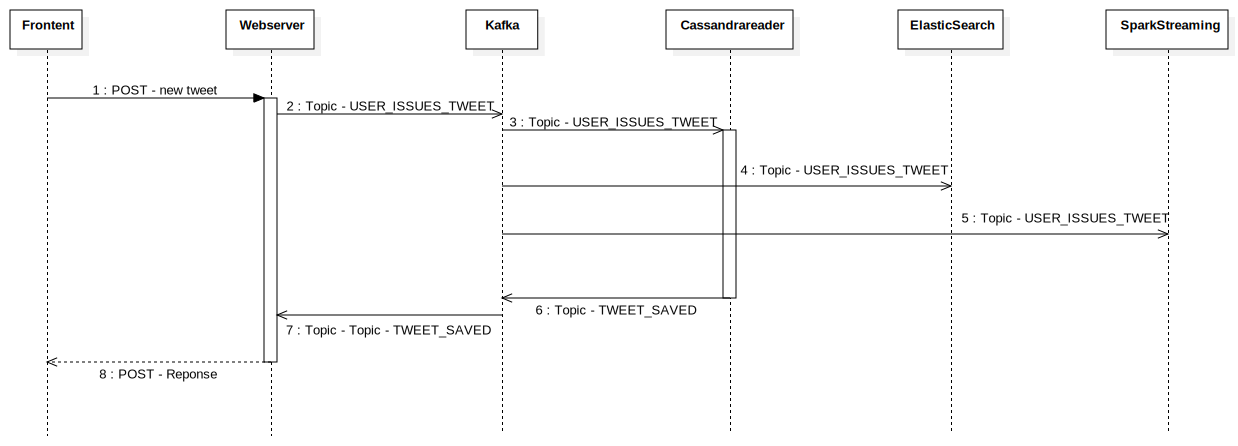
\includegraphics[width=\textwidth]{pics/useCases/IssueTweet}
	\caption{Sequence Diagram: User erstellt neuen Tweet}
\end{figure}

\subsection{User sucht einen Tweet (nach Text)}
Derzeit bietet das Hamaube-System Suchen von Tweets über Hashtags oder über den Tweet-Text.
Im Folgenden wird letzterer Fall betrachtet.
Sobald ein Nutzer im Frontend nach einem Tweet sucht, wird die Suchanfrage über Kafka an den ElasticSearch Microservice weitergereicht. Dieser vermittelt das Ergebnis der Suche als Tweet-IDs über ein Antwort-Topic, welches wiederum an den Cassandrareader geht.
Dieser liest die zugehörigen Tweets aus Cassandra und veröffentlicht das Ergebnis an den WebServer.
Gerade hier zeigt sich, dass die Meta-Information vom ursprünglichen WebServer bis zur letzten Stelle weitergereicht werden müssen, damit auch der richtige WebServer letztendlich die Tweets zur Anfrage erhält.


\begin{figure}[htbp!]
	\centering
	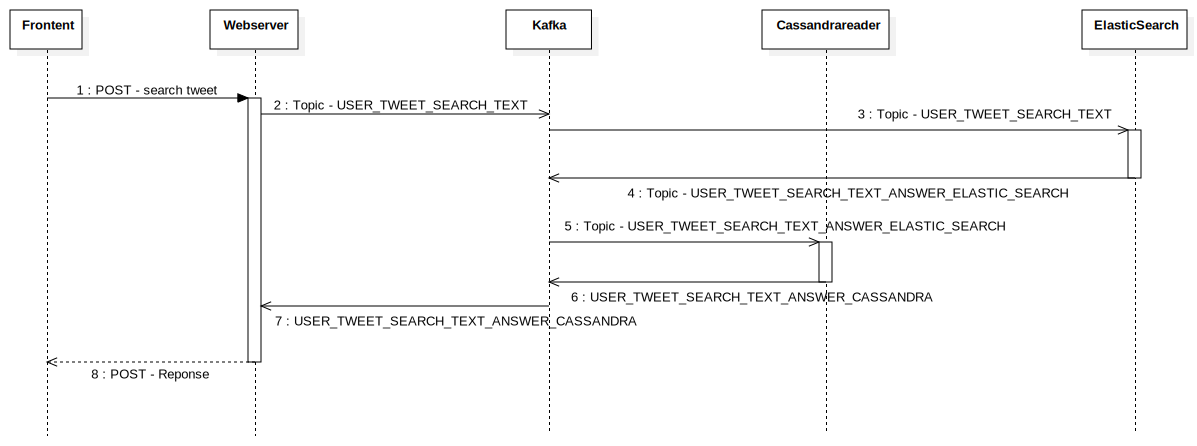
\includegraphics[width=\textwidth]{pics/useCases/SearchTweet}
	\caption{Sequence Diagram: User sucht nach einem Tweet (by text)}
\end{figure}
\chapter{Cassandra}
\label{chap:cassandra}
Cassandra ist die Quelle aller Daten von Twitter, die wir brauchen. Dazu werden die Daten direkt von der Twitter API über Kafka in Cassandra geladen und auf ein vorher für unsere Bedürfnisse zugeschnittenes Datenschema gemappt.

\section{Datenverwaltung}
Wir habe uns entschieden das Twitter Datenschema zu übernehmen. Da allerdings die Twitter Dokumentation nicht genau genug ist und nicht alle Attribute aller Datentypen übersichtlich darstellt, haben wir eine Applikation geschrieben, die sich Tweets vom Twitter Stream holt und daraus das Datenschema im JSON Format zusammenbaut. Nach dem wir die Applikation lange genug laufen lassen haben, hat sich an dem Datenschema nichts mehr geändert und wir konnten die Datentypen extrahieren.\\

\subsection{Datenschema}
\label{subsec:schema}
Nach einer eingehenden Untersuchung aller möglichen Use Cases sind wir zum Schluss gekommen, dass uns fünf Tabellen alle Funktionen bieten, die wir brauchen. Wir haben dabei zwei Tabellen für die User user\_by\_id und user\_by\_screen\_name entworfen wie man in Abbildung \ref{fig:schema} sehen kann.
\begin{figure}[htbp!]
	\centering
	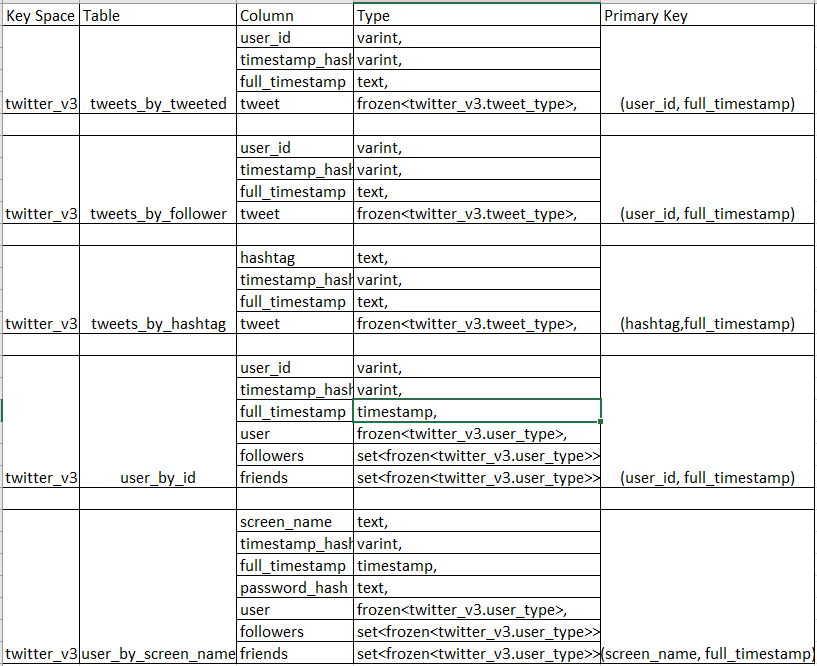
\includegraphics[scale=0.725]{pics/schema.PNG}
	\caption{Cassandra Schema}
	\label{fig:schema}
\end{figure}
Da man bei Cassandra nur über den Primary Key (PK) auf Zeilen zugreifen und Bereichsabfragen über CQL machen kann, gilt es hier den PK so zu wählen, dass alle unsere Funktionen abgedeckt sind. Deshalb haben wir neben der User-Id für user\_by\_id und dem Screen-Name des Users für user\_by\_screen\_name auch den Timestamp mit aufgenommen. Da Cassandra leider keine vollständige Konsistenz bietet, müssen wir uns selber darum kümmern. Durch den Timestamp können wir verschiedene Versionen eines Objektes auseinanderhalten und die neuste bestimmen. Somit können wir zumindest einen gewissen Grad an Konsistenz bieten. Die weiteren Attribute der beiden Tabellen lassen sich einfach erklären. Die Follower und Friends eines Users sind wichtig, um die Timeline zu erstellen. Den password\_hash in user\_by\_screen\_name brauchen wir für den Login.\\
Die anderen drei Tabellen sind dafür da, die Tweets zu speichern und alle Tweet betreffenden Anfragen zu beantworten. Auch hier haben wir wieder den Timestamp bei allen Tabellen mit in den PK aufgenommen um Teilkonsistenz zu gewährleisten. tweets\_by\_tweeted speichert alle Tweets nach der User-Id des Users ab, der den Tweet abgesetzt hat. tweets\_by\_follower hingegen speichert einmal alle Tweets nach User-Id eines jeden Followers ab. Das Konzept hier ist es, durch die mehrfache Speicherung eines Tweets die Zeit bei der Abfrage nach allen Tweets, die ein User auf seiner Timeline sehen kann, zu verkürzen. Da man einmal abgesetzte Tweets auch nicht mehr ändern kann haben wir auch kein Problem damit jedes Objekt für Änderungen wieder heraussuchen zu müssen. tweets\_by\_hashtag speichert dann die Tweets danach ab, welche Hashtags in ihnen verwendet werden. Somit können auch Abfragen über Tweets eines Hashtags effizient beantwortet werden.

\section{Cassandrareader}
Die zentrale Applikation, in der alle Funktionen und Schnittstellen umgesetzt werden ist der Cassandrareader und es ist eine modular aufgebaute in Java geschriebene Anwendung. Als Framework zur Unterstützung von verschiedenen Funktionen haben wir uns für SpringBoot entschieden. SpringBoot hat den Vorteil, dass es eine native API für Kafka besitzt, die es uns so sehr leicht ermöglicht Publisher und Subscriber für Kafka-Topics zu schreiben. So ist die Verbindung mit Kafka sehr einfach konfigurierbar und kann innerhalb von kurzer Zeit verwendet werden. In der Konfigurationsklasse werden Beans, also einzigartige Methoden, überschrieben, die die Kafka-Konfiguration für den Publisher und Subscriber erzeugen und in SpringBoot registriert sind. Diese werden für diese Konfiguration vorher in der application.properties Datei abgelegt und durch die Konfigurationsklasse eingelesen. SpringBoot erzeugt darauf aufbauend durch die Beans jeden Publisher und Subscriber nach dieser Konfiguration.
Für die Verbindung von Java zu Cassandra haben wir den DataStax Treiber genutzt \cite{DataStax}. Er bietet eine generische Schnittstelle über die man mit Cassandra über CQL kommunizieren kann. Da er gut dokumentiert ist und es sehr viele Beispiele für verschiedene Anwendungen im Internet gibt, verlief die Einarbeitung in die Nutzung des DataStax Treibers sehr schnell.
\begin{figure}[htbp]
	\centering
	
\includegraphics[scale=0.5]{pics/tech_stack.png}
	\caption{Technologie Stack des cassandrareaders}
	\label{fig:techStackCass}
\end{figure}
Alle hier und im Folgenden genutzten Bibliotheken werden über Maven eingebunden und der Applikation so zur Verfügung gestellt. Somit ist sichergestellt, dass immer die richtige Version geladen wird und keine Kompatibilitätsprobleme entstehen.

\subsection{Architektur}
Der Aufbau des Cassandrareaders ist sehr einfach gehalten wie man in Abbildung \ref{fig:archCass} sehen kann. Die Verbindung zu Cassandra wird vom Singleton CassandraConnector gemanaged. Diese Klasse stellt die Verbindung zu Cassandra her und bietet verschiedene Methoden an, Abfragen an Cassandra über CQL abzusetzen. Die eigentliche Funktion und Implementierung der Use Cases geschieht aber in den Kafka Subscribern. Dazu gibt es eine abstrakte Klasse AbstractKafkaSubscriber, die sozusagen die Infrastruktur bereitstellt. Diese besteht aus dem CassandraConnector, eine Gson-Instanz und mehreren Methoden, die die Optimierungen der Methoden aus dem Cassandra Connector darstellen, wie z.B. Batch-Queries und asynchrone Queries. Die Gson-Instanz kommt von der Google Gson Bibliothek, die für die JSON Konvertierung von Java Klassen zuständig ist. Sie wird in den abgeleiteten Klassen so benutzt, dass Kafka-Anfragen direkt in POJOs (Plain Old Java Objekte) gemappt werden, aus denen man dann alle relevanten Informationen bekommt. In den abgeleiteten Klassen wird dann auch die eigentliche Funktion eines Use Cases implementiert.
\begin{figure}[htbp]
	\centering
	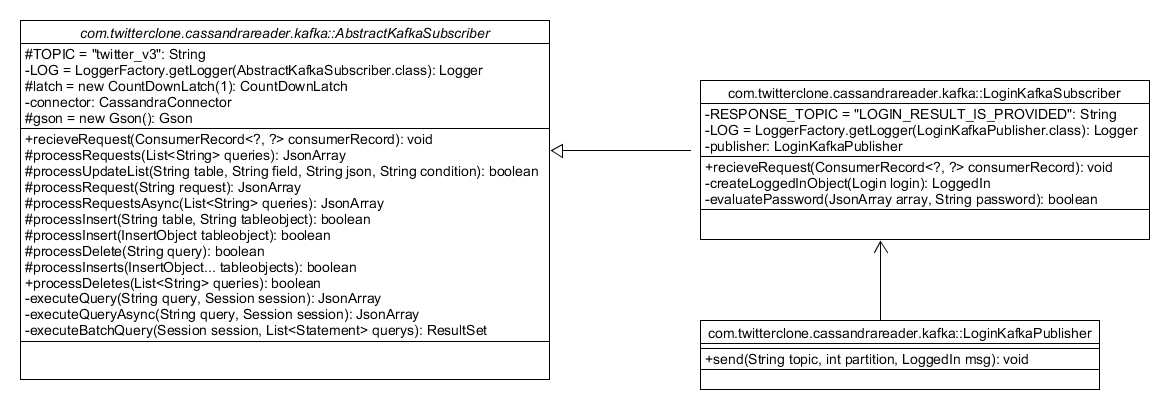
\includegraphics[scale=0.3]{pics/cassandrareader_architecture.png}
	\caption{Architektur der Publisher und Subscriber am Beispiel Login}
	\label{fig:archCass}
\end{figure}
Alle möglichen Anfragen und Antworten über Kafka sind als Java Klassen modelliert und können über Getter-Methoden abgefragt werden. Jeder der abgeleiteten Subscriber besitzt einen Publisher, über den die Antwort, durch Gson konvertiert, wieder versendet werden kann. Die Konfigurationsparameter sind in der Datei application.properties abgelegt und werden in den einzelnen Klassen angesprochen.


\section{Use Cases}
\label{sec:usecase}
Bei der Identifizierung der Use Cases, die für Cassandra relevant sind, haben wir uns für die Funktionen entschieden, die für einen Twitter-Client nach MVP-Prinzip (Minimal Viable Product) notwendig sind. Dabei haben wir vor allem die dazu gehören folgende Funktionen identifiziert:
\begin{itemize}
	\item Registrierung von User
	\item Anmelden von Usern
	\item Abfragen von Usern
	\item Absenden/Speichern von Tweets
	\item Abrufen der Timeline
	\item Folgen von Usern
\end{itemize}
Diese Schnittstellen machen es möglich die Grundfunktionen, also das Erstellen eines Users, das Anmelden des Users, das Senden und Lesen von Tweets über die Timeline von außen über vordefinierte Kafka Nachrichten anzusprechen.
Als weitere Schnittstellen für erweiterte Funktionen haben wir eine API für Volltextsuche über Elasticsearch gebaut, die die normale Volltextsuche aber auch Autocompletion unterstützt.\\

\subsection{Registrierung von Usern}
Die Registrierung von Usern bringt einen direkten Zugriff auf die Datenbank mit sich. Zunächst muss der User seine Anmeldedaten in unserem Frontend hinterlegen. Schickt er diese, bekommt der Cassandrareader über eine Zwischenstelle eine Nachricht über Kafka auf dem Topic ``USER\_ISSUES\_ REGISTRATION". Diese Nachricht enthält alle relevanten Daten wie Name, Username, Hashwert des Passworts, etc. die das System braucht um den User anzulegen. Der Cassandrareader reagiert auf diese Nachricht, indem er den User in den in Abschnitt \ref{subsec:schema} genannten Tabellen für die User ablegt. Der Cassandrareader schickt eine Nachricht auf dem Topic "REGISTRATION\_RESULT\_PROVIDED" als Bestätigung zurück, ob der User erfolgreich in beide Tabellen eingetragen wurde oder nicht. Basierend auf dieser Nachricht wird im Frontend angezeigt, ob die Registrierung erfolgreich war.

\subsection{Anmelden von Usern}
Die Anmeldung von Usern geschieht über den einzigartigen Username und ein selber gewähltes Passwort. Diese Informationen werden vom Frontend weitergeleitet und kommen beim Cassandrareader in einer Kafka Nachricht auf dem Topic ``USER\_ISSUES\_LOGIN" an. Diese Nachricht enthält nur den Username und das gehashte Passwort. Das gehashte Passwort wird mit dem verglichen, das in der Tabelle user\_by\_screen\_name gespeichert ist. Auch hier findet sich nur ein Hashwert des Passworts. Sind die Werte gleich, so gibt es hier eine Übereinstimmung und der Login kann genehmigt werden. Als Bestätigung dieses Vorgangs schickt der Cassandrareader eine Nachricht zurück, in der es eine Boolean Feld für das Login Ergebnis gibt. War der Login erfolgreich wird das Feld true, sonst false. Diese Nachricht wird vom Cassandrareader wieder über das Topic "LOGIN\_RESULT\_IS\_PROVIDED" verbreitet und somit auch an das Frontend weitergeleitet, das das Ergebnis darstellt und darauf reagiert.

\subsection{Abfragen von Usern}
\label{subsec:Userabfrage}
Das Abfragen von Usern braucht man vor allem, wenn man die Seite eines Users mit allen seinen Informationen aufrufen möchte. Dazu verarbeitet der Cassandrareader Nachrichten auf dem Topic "USER\_OPENS\_USER\_PAGE" in der eine User-Id angegeben ist, so dass er eine Abfrage auf Cassandra startet, in der er den User aus user\_by\_id abfragt. Dieser User wird dann als JSON in einer Kafka Nachricht über das Topic ``USER\_PAGE\_ENTRIES\_ PROVIDED" wieder verbreitet. So können die Information dann vom Frontend dann z.B. als User Seite verarbeitet werden.\\
Ein ähnlicher Use Case ist die Suche nach Usern. Der Cassandrareader bekommt auf dem Topic ``USER\_SEARCH\_ISSUED" eine Nachricht mit einem Usernamen. Da die Tabelle user\_by\_screen\_name nach Usernamen filterbar ist, kann der Cassandrareader eine effiziente Abfrage auf der Tabelle ausführen, die alle mit dem Namen aus der Nachricht übereinstimmenden User zurückgibt und danach den besten möglichen auswählt. Dieser wird dann in einer Nachricht auf dem Topic "USER\_SEARCH\_RESULT\_ PROVIDED" zurückgeschickt und kann dann weiterverarbeitet werden.

\subsection{Absenden/Speichern von Tweets}
\label{subsec:Tweetabfrage}
Das Absenden von Tweets ist im Endeffekt nichts anderes als ein Einfügen eines Tweets in die Datenbank. Da wir hier aber nicht mit einer relationalen Datenbank arbeiten, muss man Einfügen vor allem auf die Konsistenz des Datenschemas achten. Jeder Tweet muss nach dem Schema unabhängig voneinander in jedem der drei Tweet Tabellen richtig abgelegt werden. Dafür bekommt der Cassandrareader das Tweet Objekt über Kafka auf dem Topic ``USER\_ISSUES\_TWEET" zugeschickt. Dieses Objekt wird dann mit dem Absender als User in die Tabelle tweets\_by\_tweeted eingefügt. Zusätzlich lesen wir alle Hashtags des Tweets aus und speichern ihn in der Tabelle tweets\_by\_hashtag noch einmal für jeden Hashtag, das beschleunigt das Auslesen nach Hashtags. Als letztes wird der Tweet auch noch einmal in der Tabelle tweets\_by\_follower abgespeichert, in der jeder Tweet eines Users für jeden User, der ihm folgt, abgespeichert werden. Dafür müssen natürlich zunächst erst einmal alle Follower des Absenders abgefragt werden, bevor der Tweet für sie gespeichert werden kann. Diese redundante Speicherung von Tweets beschleunigt das Auslesen für spezifische und oft gebrauchte Use Cases ungemein und hat für uns die damit einhergehenden Performance Nachteile beim Speichern von Tweets überwogen. Der Cassandrareader führt diese Einfüge Operationen durch und bestätigt über Kafka auf dem Topic "TWEET\_SAVED", ob das Speichern erfolgreich war oder nicht.


\subsection{Abrufen der Timeline}
\label{subsec:Timeline}
Das Abrufen der Timeline ist einer der zentralen Use Cases unserer Anwendung, da sie der erste Teil ist, den User innerhalb unserer Anwendung sehen und die Basis für jede Aktion nach dem Anmelden ist. Die Timeline eines Users besteht aus den Tweets aller User, denen der eingeloggte User folgt. Daher müsste man diese User zunächst aus der Datenbank abfragen und dann für jeden einzelnen eine einzelne Abfrage starten. Um uns diesen Umweg zu sparen, pflegen wir die Tabelle tweets\_by\_follower. Somit können wir, um die Timeline aufzurufen, einfach eine Abfrage auf diese Tabelle ausführen und bekommen somit direkt den Inhalt der Timeline. Wir nehmen dabei für das Speichern von Tweets mehr Datenbankzugriffe und Redundanzen in Kauf, wie in Unterabschnitt \ref{subsec:Tweetabfrage} beschrieben, um das Auslesen so effizient wie möglich zu gestalten. Die so abgefragten Tweets werden danach als JSON verpackt und auf dem Topic "TIMELINE\_ENTRIES\_PROVIDED" verbreitet. So kann die Nachricht zum Frontend propagiert werden, das dann die Timeline anzeigt.


\subsection{Folgen von Usern}
Das Folgen von Usern bestimmt vor allem den Aufbau der Timeline, da hier, wie in Unterabschnitt \ref{subsec:Timeline} erwähnt, alle Tweets der gefolgten User angezeigt werden. Um das Folgen von Usern umsetzen zu können, erhält der Cassandrareader einer Nachricht auf dem Topic ``USER\_WANTS\_TO\_FOLLOW\_ USER", in der die User-Id des anderen Users und des eigenen steht. Followers werden in unserem Datenschema für jeden User als Liste gespeichert, einmal alle User, denen ein User folgt, und alle User, die einem User folgen. Jeder Eintrag für einen User in den Tabellen user\_by\_id und user\_by\_screen\_name enthält beide Listen. Außerdem enthält das User Profil einen Follower Count und eine Friends Count, der die Anzahl User zählt denen man selber folgt. Der Cassandrareader führt auf beiden Tabellen für jede Folgen Anfrage folgende Aktion durch. Er erhöht beim eigenen User den Friends Count und beim User, dem gefolgt werden soll, den Follower Count. Danach wird das User Profil des Users, dem gefolgt werden soll, in die Friends Liste des anfragenden Users hinzugefügt und das Profil des anfragenden Users in die Follower Liste der zu folgenden Users. Geschieht das alles ohne Fehler bestätigt der Cassandrareader die Anfrage auf dem ``USER\_FOLLOWS\_USER" Topic positiv.

\chapter{Search Engine}
Die Twitter-Klon Applikation soll mit einer Suchfunktion erweitert werden. Diese Suchfunktion wird mit einem Such-Service umgesetzt, der auf der Elasticsearch-Engine basiert. Elasticsearch setzt auf Apache Lucene auf, einer in Java geschriebenen Bibliothek für die Volltextsuche. Es ist open-source, dokumentenorientiert, in Java geschrieben und lässt sich über einen REST-API ansprechen. Damit ist es ein guter Kandidat für unser Use-Case.

\section{Zielsetzung}
Das Ziel des Suchservices ist die Ausgabe von \textit{best-match} Ranglisten über eine Tweets-Sammlung zu erstellen, indem man nach bestimmten Benutzern, Tags und Freitexteingaben sucht. Als Erweiterung der Suchfunktion wird ein Text-Vervollständigung Feature erstellt, das beim Suchen nach Tweets passende Vorschläge liefert. Und zum Schluss sollen ausgewählte Datensätze, mit Hilfe eines Analyse- und Visualisierungstools, auf der Homepage als eine Grafik angezeigt werden. 

\section{Vorgehen}
Zuerst wird eine \textit{Elasticsearch-Service} Architektur angefertigt. Diese stellt nur ein Teil der \textit{Twitter-Klon} Umsetzung und behandelt die Kommunikation zwischen \textit{Elasticsearch}, \textit{Elasticsearch-Service} wie den \textit{Kafka-Topics}. Nachfolgend wird Elasticsearch entsprechend der \textit{Twitter-Klone} Applikation konfiguriert und für die Datenaufnahmen vorbereitet. Infolgedessen wird der Such-Service implementiert, der \textit{Elasticsearch} mit den \textit{Kafka-Topics} verbindet und für den Datenaustausch zuständig ist. Anschließend werden Datenvisualisierungen mit Hilfe von \textit{Kibana} angefertigt. Zum Schluss wird der Elasticsearch Abschnitt mit einem Fazit beendet.

\section{Service Design}
Der komplette Nachrichtenaustauch der \textit{Twitter-Klon} Applikation wird mit einem skalierbaren und performanten Messaging-Service umgesetzt, nämlich \textit{Apache Kafka}. Dieser, bietet die Möglichkeit, mit Hilfe der Nachrichten-Topics den Overhead an Kommunikation zwischen den Services zu verringern, die Services von einander zu entkoppeln und die Daten parallel zu verarbeiten.
Diese Eigenschaft ermöglicht das Entkoppeln des Such-Service‘es von dem Restsystem, sodass die Suche unabhängig von den Schnittstellen der heterogenen Klienten bedient werden kann. 
Dafür wurden drei Topics erstellt und ein Datenformat vereinbart, das langfristig alle unsere Wünsche abdecken soll. Die Such-Service Use-Cases sind in drei Gruppen eingeteilt, die mit Hilfe von drei Kafka-Topics realisiert wurden: Neue Dokumente indexieren/abspeichern, Anfragen empfangen und Anfragen beantworten.
%\captionsetup{justification = raggedright,singlelinecheck = false}
\begin{figure}[htbp!]
  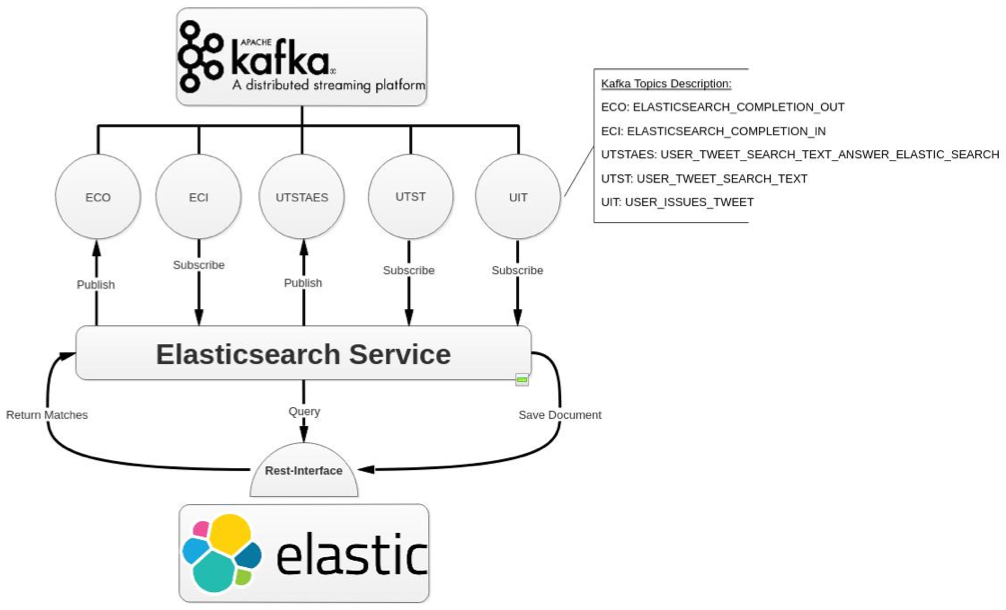
\includegraphics[scale=0.8]{material/architecture/Elasticsearch.png}
  \caption{Elasticsearch Service Architectur}
  \label{fig:ESA}
\end{figure}

Der Such-Service meldet sich an den entsprechenden Kafka-Topics an, öffnet ein Datenstrom und empfängt Nachrichten mit den Speicher-, Suchkriterien, sowie der dazugehörigen Benutzerkennung. Um den Speicherplatz optimal zu nutzen, werden aus der Nachricht nur für die Suche relevante Felder ausgelesen und an die Elasticsearch REST-Schnittstelle weitergeleitet, wie z.B. der Text, die Benutzerkennung, die Tags und der Zeitstempel.  

Das Verschicken der Nachrichten über unsere Applikation durchläuft den \textit{UIT} Topic, dieser bietet jedem Abonnenten den Zugriff auf die neu eingetroffenen Mitteilungen. Der Elasticsearch-Suchservice ist einer der bestehenden Abonnenten des \textit{UIT} Topics und bereitet die neu eingetroffenen Nachrichten für die Weiterleitung und das Speichern des Inhalts in Elasticsearch. Die, mit Metainformation bestückten, Nachrichten laufen eine Transformation durch wie Filterung, Umbenennung und Umstrukturierung, um der Elasticsearch erwarteten Datenstruktur zu entsprechen und Speicherplatz zu sparen. 

Für die Suchfunktion werden die Topics \textit{UTST} und \textit{UTSTAES} genutzt. Über den \textit{UTST} werden Suchanfragen entgegengenommen und in eine Elasticsearch-Rest-Anfrage umgeformt. Die Suchanfrage kann von dem Suchservice auf verschiedene Weise durchgeführt werden. Zum Beispiel durch eine Term-, Bollean-, Match-, Multimatch- und Match-Phrase- Suche. Jede Abfrageart, kann im bestimmten Fällen vorteilhaft ausgenutzt werden und kann Fallspezifisch eingesetzt werden. 
Das Suchergebnis wird anschließend als eine sortierte Identifikationsliste zu enthaltenen Nachrichten auf dem \textit{UTSTAES} Topic hinterlegt. Damit wäre die Suche beendet und das weitere Geschehen des Suchergebnisses den \textit{UTSTAES} Abonnenten überlassen.

Die Suchvervollständigung verhält sich ähnlich der Suchfunktion. Der Suchservice kommuniziert über die Topics \textit{ECI} und \textit{ECO}, die vervollständigung Anfragen für die Benutzereingabe publizieren und mögliche Eingabewünsche entgegennehmen. Die Eingabewünsche könne mit Hilfe der Elasticsearch Vervollständigung oder durch die nGrams-Implementation umgesetzt werden. Diese Ansätze sind in der Granularität, Umsetzung, Laufzeit und Speicherbedarf unterschiedlich und könne Fallabhängig ausgetauscht werden. 


\section{Elasticsearch Konfiguration}
Elasticsearch funktioniert \textit{out of the box}, das heißt, man muss den Service nur starten und das Indexieren, wie das Suchen der Dokumente funktioniert reibungslos. Im Gegensatz zu den relationalen Datenbanken ist eine Schema Definition für Elasticsearch nicht notwendig. Obwohl ein Schema nicht gefordert ist, ist es höchst ratsam dieses zu deferieren, denn das \textit{Type-Matching} der Felder wird ansonsten nach dem \textit{Best Guess} Prinzip erstellt und kann unter umstanden zum unerwünschten Verhalten führen.

\subsection{Index Settings}
Die \textit{out of the box} Fähigkeit von Elasticsearch ist toll zum Ausprobieren, jedoch ist es für den Betrieb ungeeignet, da die Einstellungen für die bestmögliche Skalierung von Elasticsearch, wie das Durchsuchen der Texte immer von der Domäne abhängt. Falsche oder keine Anpassung, kann die Skalierungsmöglichkeiten von Elasticsearch drastisch senken und damit den Betrieb unerwartet unterbrechen. Des Weiteren ist die Anpassung der Textvorverarbeitung eine Kernaufgabe jeder Such-Engine, dementsprechend sollte man sich besonders sorgfältig um diese Aufgabe kümmern, sodass alle relevanten Ergebnisse ermittelt und in einer passenden Ordnung dem Nutzer vorgelegt werden können.

\subsection{Sharding \& Replication}
Zuerst wird der Elasticsearch Index auf Shards und Replicas aufgeteilt. Damit enthält ein Shard eine Teilinformation oder ein Replikat der Teilinformation des Indexes, der auf unterschiedliche Hardware aufgeteilt werden kann. Obwohl die Verschiebung des Shards Knotenübergreifend realisiert werden kann, kann dieser nicht in zwei neue Shards gespalten werden, wenn die Hardware an ihre Grenzen stößt. Damit ist ein Shard die Skalierungseinheit des Indexes und muss sorgfältig gewählt werden. Der uns gegebene Elasticsearch Cluster arbeitet nur auf einem Knoten, dementsprechend ist der Skalierungsfaktor von fünf genug um zukunftssicher den Index bis auf fünf weitere Knoten aufteilen zu können. Der Replikationsfaktor beschreibt wie viele Replikate für einen Shard erstellt werden. Für eine Einstellung aus fünf Shards und einem Replikat entsteht eine Gesamtdatenmenge von 10 Shards. Daraus folgt ein immenser Anstieg an Speicherverbrauch für jeden nächsten Replikat eines Shardes. Die Replikate bieten im Gegensatz die Ausfallsicherheit und die Performance Steigerung der Lesezugriffe. Da die Performance und die Ausfallsicherheit für jeder skalierbare Applikation Kernkriterien sind, kann Elasticsearch diese bei Bedarf im laufenden Betrieb durch neue Replikate stärken. In unserem Fall steht nur einen Knoten zur Verfügung, dementsprechend folgt kein Anstieg der Performance wie Ausfallsicherheit mit Hilfe der Replikation.
% Bild  mit Reploikation der Shards und Replikas auf Knoten.
\\\\
\textbf{Initiale Index Einstellungen}
\begin{lstlisting}[language=json,firstnumber=1]
{
  "twitterindex": {
    "settings": {
      "index": {
        "number_of_shards": "2",
        "number_of_replicas": "0",
        "refresh_interval": "1s",
        "provided_name": "twitterindex",
        "creation_date": "1529674155106",
        ...
        "uuid": "wOHQnu5GQjOs7iP-Cv-_MQ",
        "version": {
          "created": "6020399"
        }
      }
    }
  }
}
\end{lstlisting}

\subsection{Textvorverarbeitung}
Als nächstes wird der Textvorverarbeitungsprozess definiert. Unter dem Schlüssel \textit{Analyzer} wird ein \textit{Custom Analyzer} und die dazugehörigen Vorverarbeitungsschritte erstellt. Dieser wird innerhalb Elasticsearch aufbewahrt und mit Funktionalität belegt. Der Analyzer zerlegt den Text mit dem \textit{Partial Word Tokenizer} in Tokens nach einem bestimmten Muster, nämlich nach einem Leerzeichen, nach einem Großbuchstaben Anfang und nach einer Zahl.
Dieser Zerlegungsschritt erfüllt die gegebenen Anforderungen, könnte aber auf Kosten des Speicherplatzes durch den mächtigeren \textit{Edge NGram Tokenizer} ausgetauscht werden. Nachfolgend laufen die Tokens eine Transformationskette durch. Zuerst werden die Tokens in Kleinbuchstaben umgewandelt, auf den Wortstamm zurückgeführt und Worte mit geringen Informationsgehalt, sowie verboten Worte entfernt. Zuletzt werden die Worte mit ähnlicher Bedeutung wie \textit{Universität Hamburg} und \textit{UHH} in Synonymlisten zusammengefasst und als gleichgültig behandelt. 
\\\\
\textbf{Analyzer}
\begin{lstlisting}[language=json,firstnumber=1]
"analyzer": {
...
  "my_analyzer": {
    "filter": [
      "my_tokenizer",
      "lowercase",
      "my_stemmer",
      "english_possessive_stemmer",
      "my_stop",
      "my_synonym"
    ],
    "type": "custom",
    "tokenizer": "standard"
  },
...
}
\end{lstlisting}

\subsection{Data Mapping}
Zuletzt braucht Elasticsearch ein Datenschema, um die automatische Fehleinschätzung des Mappings zu vermeiden. 
Elasticsearch baut einen Suchindex auf, der Dokumentenbasiert in einem JSON Format abgespeichert wird. Das Mapping garantiert eine Typenzusicherung wie das Format, der zu speichernden Felder und Dokumente. Zum Beispiel das Datumformat, das Regionsunabhängig vor dem Abspeichern von Elasticsearch normalisiert wird oder das Textfeld, das man mit bestimmten Eigenschaften und Funktionen anreichert, um das gewünschte Verhalten zu realisieren. 
Der Text, kann als \textit{Keyword} abgespeichert werden, das Eins-zu-eins durchsucht wird oder ein \textit{Text}, das mit Hilfe der Volltextsuche komplexen Suchkriterien umsetzen kann.
Das Elasticsearch Mapping für den Twitter-Klon definiert ein Dokumentenformat mit sieben Felder: id, message, tags, users, timeStamp, userLocation und userLocationCompletion. Für die Suche sind die Felder \textit{message}, \textit{tags} und \textit{use} relevant, diese werden vom Type \textit{Keyword} und \textit{Text} gespeichert. Das Feld \textit{timeStamp} wird auf ein \textit{Long} projiziert und für die Datenvisualisierung mit Kibana genutzt, um die wöchentlichen Trends anzuzeigen. Das Feld \textit{userLocation} hält die vom Benutzer eingetragene Standort, der mit der Textvervollständigungsinformation von Elasticsearch angereichert und durch das Feld \textit{userLocationCompletion} beschrieben. Zum Vergleich wird das Feld \textit{userLocation}  zusätzlich mit dem \textit{nGram Analyzer} belegt, um die Text-Verfollständigung von Elasticsearch mit der \textit{nGram} Methode vergleichen zu können.  
\\\\
\textbf{Mapping}
\begin{lstlisting}[language=json,firstnumber=1]
"userLocation": {
  "type": "text",
  "analyzer": "nGram_analyzer",
  "search_analyzer": "nGram_search_analyzer"
},
"userLocationCompletion": {
  "type": "completion",
  "analyzer": "simple",
  "preserve_separators": true,
  "preserve_position_increments": true,
  "max_input_length": 50
},
\end{lstlisting}


\section{Search Service}
Die Implementation des Such Service wird mit Java und Spring realisiert. Spring ist ein weit verbreitetes und etabliertes Enterprise Framework für Java. Dieses besitz eine große Palette an Werkzeigen, die das Arbeiten in einer heterogenen Umgebung stark vereinfachen. Daher eignet sich Spring besonders gut für unseren Anwendungsfall. Für den Nachrichtenaustausch zwischen Apache Kafka, Elasticsearch und dem Suchservice wird, die von Spring entwickelte \textit{Spring for Apache Kafka} und die von Elasticsearch angebotene \textit{Elasticsaerch Rest Client} Bibliotheken genutzt.
Die interne Logik des Suchservices wird von den Java Beans umgesetzt, die im Springkontext auf dem Apache Tomcat Application Server ausgeführt werden und die gewünschte Such-Funktionalität umsetzen.

\subsection{Such-Interface}
Um die Kommunikation und Fähigkeiten des Such Services übersichtlich zu gestalten, wird ein Interface mit den gewünschten Anfragen erstellt und anschließend implementiert. 

\begin{enumerate}
  \item über die Tags
  \item über die referenzierten Benutzer
  \item über angegebenen Standortnamen mit der Textvervollständigung
  \item über die Term-Suche auf den Tweet-Text
  \item über die Volltextsuche auf den Tweet-Text
  \item über den Text wie den Benutzet Standortnamen
  \item über einen Zeitraum
  \item über einen Zeitraum mit Benutzer und Tag Präferenz 
\end{enumerate}

\subsection{Such-Implementation}
Elasticsearch bietet eine JSON-ähnliche domänenspezifische Sprache, mit der man Abfragen ausführen kann. Dies wird als \textit{DSL Query} bezeichnet. Die Abfragesprache ist ziemlich umfassend und bietet komplexe Filter und Aggregation Möglichkeiten. Die Anfragen des Suchservices sind ausgelegt die wichtigsten Anfragemöglichkeiten von Elasticsearch darzustellen. Es werden \textit{term}, \textit{match}, \textit{multi match}, \textit{match phrase}, \textit{bool}, \textit{compleation} und \textit{aggregation} Anfragen behandelt. 
\\\\
\textbf{Suchen nach Tags}
\begin{lstlisting}[language=json,firstnumber=1]
{
  "query": {
    "terms": {
      "tags.keyword": "?"
         }
    }
}
\end{lstlisting}

\textbf{Suche nach Referenzierten Benutzer}
\begin{lstlisting}[language=json,firstnumber=1]
{
  "query": {
    "terms": {
      "users.keyword": "?"
    }
  }
}
\end{lstlisting}

Die Tag- und Benutzersuche wird mit der Term-Suche umgesetzt, diese sucht nach Dokumenten, die genau, die im angegebenen Feld angegebenen Begriffe enthalten. Die Tweets werden entsprechend den TF/IDF Relevanz sortiert und präsentiert.  
\\\\
\textbf{Textvervollständigung nach Standortnamen}
\begin{lstlisting}[language=json,firstnumber=1]
{
  "suggest": {
    "location_suggest": {
      "prefix": "?",
      "completion": {
        "field": "userLocationCompletion",
        "fuzzy": {
          "fuzziness": 1
        }
      }
    }
  }
}
\end{lstlisting}
Der Textvervollständigung bietet Funktionen zur automatischen Vervollständigung. Es werden Vorschläge wehrend des Tippens einer Anfrage getätigt und führt schneller zu relevanten Ergebnissen. Durch die zusätzliche \textit{fuzzy} Eigenschaft der Abfrage werden zusätzlich Tippfehler abgefangen um die Suche den Nutzer angenehmer zu gestalten.
\\\\
\textbf{Term-Suche auf den Tweet-Text}
\begin{lstlisting}[language=json,firstnumber=1]
{
  "query": {
    "match": {
      "message": "?"
    }
  }
}
\end{lstlisting}

\textbf{Volltextsuche auf den Tweet-Text}
\begin{lstlisting}[language=json,firstnumber=1]
{
  "query": {
    "match_phrase": {
      "message": {
        "query": "?",
        "slop": 1
      }
    }
  }
}
\end{lstlisting}

Die Suche über den Textkörper eines Tweets kann auf zwei Arten getan werden. Im ersten Fall wird eine Match-Suche \textit{metch} durchgeführt, diese normalisiert die Suchterme, verknüpft sie mit \textit{OR} und durchsucht den Textkörper nach Suchbegriff-Treffern. Im zweiten Fall nutzt man die zusammenhängende Suchanfrage \textit{phrase match}, welche im Gegensatz zu \textit{match} die Terme mit \textit{AND} verknüpft und eine Einschränkungen mitbringt, nämlich die Ordnung der Suchterme im Textkörper. Um die Suche flexibler zu gestalten, kann sie aufgeweicht werden, indem man die akzeptable Entfernung der Suchterme mit der \textit{Slope} Eingeschalt beeinflusst. In unseren Fall erlaubt diese eine Entfernung von einem Wort zwischen den Suchbegriffen.

\textbf{Standortabhängige Tweets}
 \begin{lstlisting}[language=json,firstnumber=1]
 {
  "query": {
    "multi_match": {
      "query": "?",
      "fields": [
        "message",
        "userLocation"
      ]
    }
  }
}
\end{lstlisting}

Die \textit{multi match} Abfrage sucht nach Nachrichten, dessen Inhalt einen Ort verweist und der Autor sich in dieser Region befindet. Diese Abfrage verhält sich wie \textit{match}, jedoch über eine Menge von Feldern.
\\\\
\textbf{Suche Tweets über den Zeitraum mit referenzierte Benutzer zuerst}
 \begin{lstlisting}[language=json,firstnumber=1]
{
  "query": {
    "bool": {
      "must": {
        "terms": {
          "tags": "?"
        }
      },
      "filter": {
        "range": {
          "timeStamp": {
            "gte": "now-1d/d",
            "lt": "now/d"
          }
        }
      },
      "should": [
        {
          "term": {
            "users": "?"
          }
        }
      ]
    }
  }
}
\end{lstlisting}
Diese Suchanfrage führt ein neues Konzept der \textit{bool} Anfrage, die aus mehreren Komponenten besteht. Die Suche besteht aus erforderlichen Feld-Treffern wie den optionalen Feld-Treffern. Daraus ergibt sich eine Rangordnung aus den relevanten Ergebnissen. Zuletzt läuft die Liste einen Zeitfilter durch um den Zeitraum einzuschränken. 
\\\\
\textbf{Top Tweets für die letzten sieben Tage }
 \begin{lstlisting}[language=json,firstnumber=1]
{
  "aggs": {
    "top_tags": {
      "significant_terms": {
        "field": "tags",
        "size": 10
      }
    }
  },
  "query": {
    "bool": {
      "must": [
        {
          "match_all": {}
        },
        {
          "range": {
            "timeStamp": {
              "gte": "now-7d/d",
              "lt": "now/d"
            }
          }
        }
      ]
    }
  }
}
\end{lstlisting}
Diese Anfrage ist zuständig für die Visualisierung in Kibana. In diesem Fall wird mit Hilfe der \textit{bool} Anfrage und der Elasticsearch-Aggregation, die am häufigsten verwendeten Tag über den Datensatz von sieben Tagen erarbeitet.  
\\\\
\section{Visualisierung mit Kibana}
Die Visualisierungsmöglichkeiten von Kibana sollen es ermöglichen große Datenmengen zu analysieren unterstützt durch flexible Filter. Es bietet Echtzeit-Analyse von Daten, individuell konfigurierbare Visualisierung, dynamische Dashboards und Browserbasiertes Interface, das Plattformunabhängige funktioniert.\\\\
Die Kibana Visualisierungen basieren auf den Aggregationsmöglichkeiten von Elasticsearch. Dieses aggregiert über den Elasticsearch Indexinhalt und erstellt Grafiken, die in HTML eingebunden werden können. Zur Verfügung stehende Visualisierungstypen: Area Chart, Data Table, Line Chart, Markdown Widget, Mertric, Pie Chart, Tile Map, Vertical Bar Chart.
%\captionsetup{justification = raggedright,singlelinecheck = false}
\begin{figure}[htbp!]
  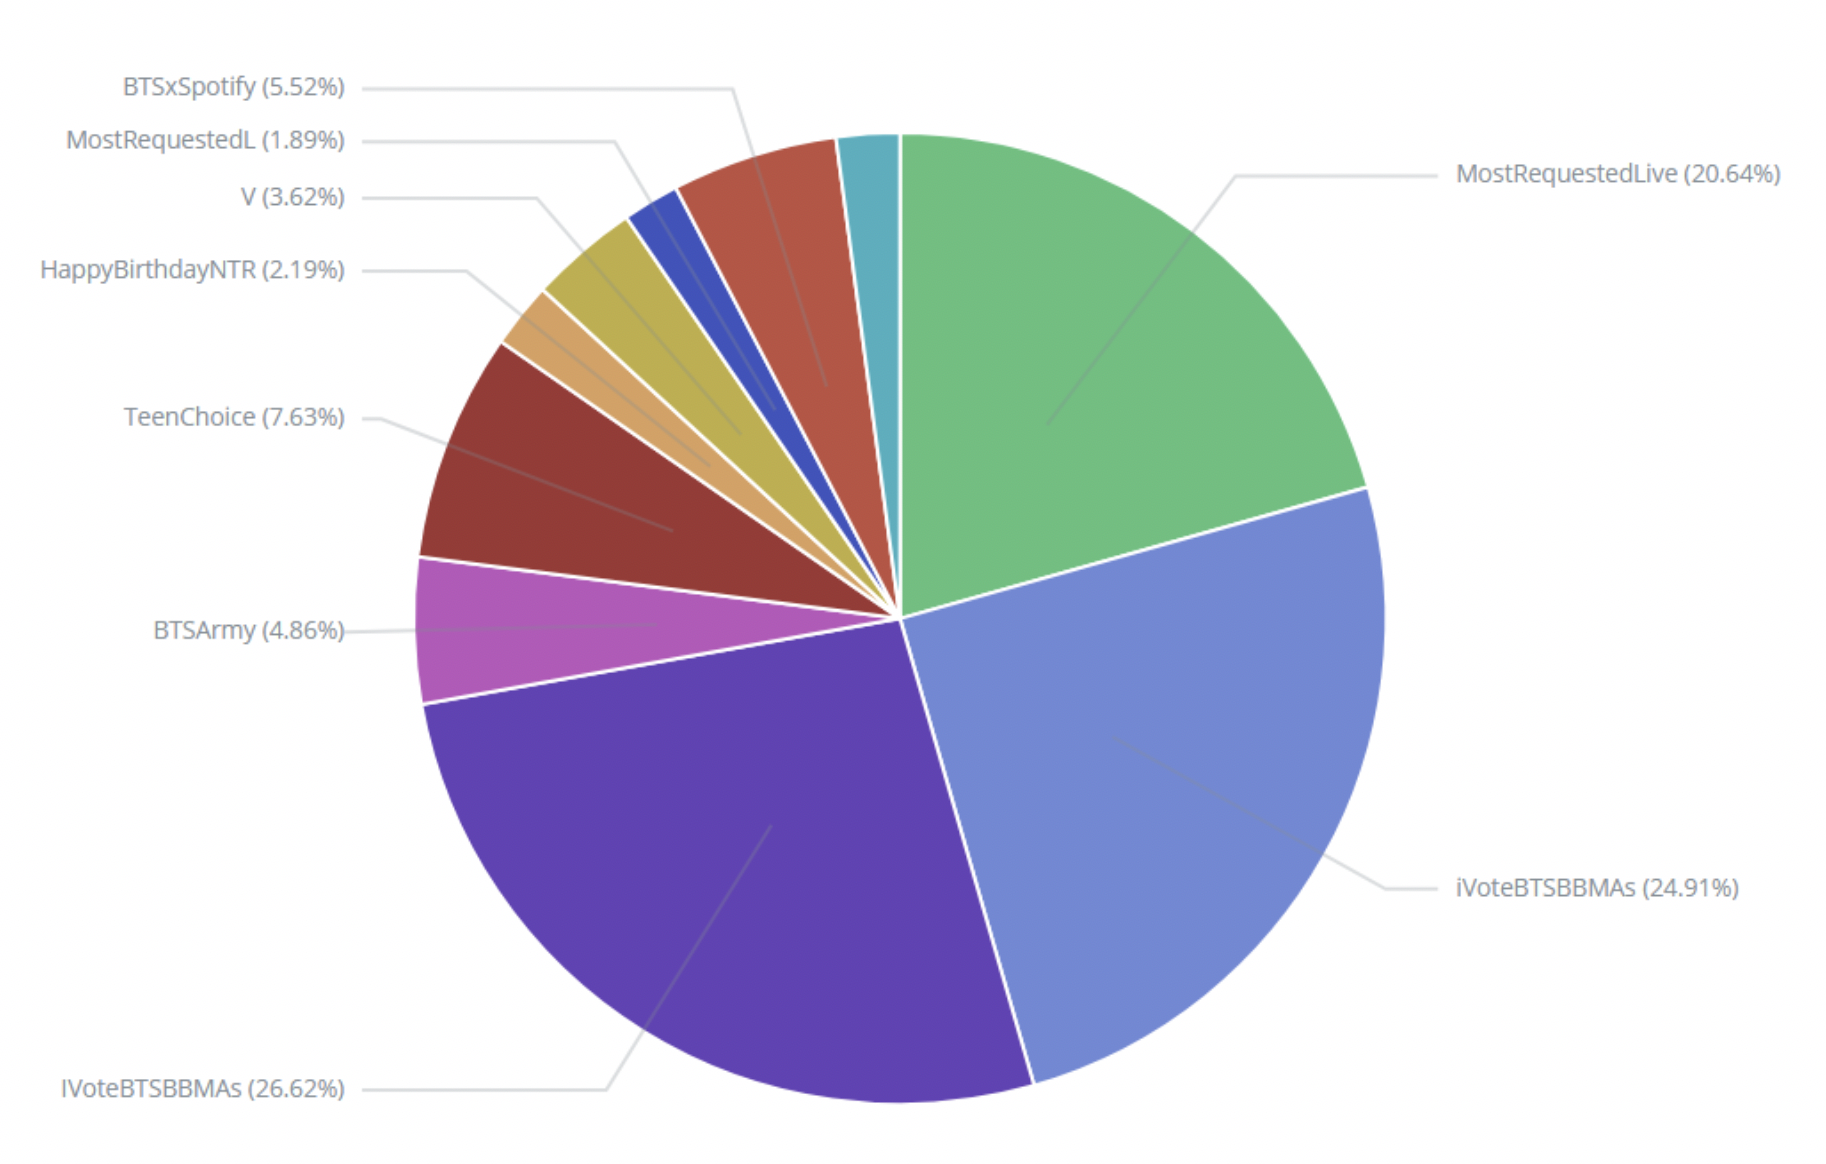
\includegraphics[scale=0.4]{material/architecture/kibana.png}
  \caption{Kibana Analyseplattform} 
  \label{fig:Kibana}
\end{figure}

\section{Fazit}
\subsection{Suchfunktionalität}
Jede moderne Software bietet eine Möglichkeit nach Daten zu suchen. Mit Hilfe von Elasticsearch kann eine einfache Suche nach einer Website oder einem Dokument innerhalb einer Sammlung implementiert werden. Anschließend kann eine Rechtschreibprüfung hinzugefügt werden. Höchstwahrscheinlich ist eine fuzzy Suche und automatische Vervollständigung nötig, möglicherweise sogar während der Eingabe. Da die Relevanz wichtig ist, können fortgeschrittene Ranking-Schemata erstellt werden. Zum Beispiel können Suchergebnisse basierend auf dem Standort, Zeit sowie des Benutzers ausgeführt werden. Und um zu wissen, was die Benutzer tatsächlich tun, kann die Nutzung der Software protokolliert und gespeichert werden für die spätere Analyse der Nutzerdaten.
\newline
Damit ist Elasticsearch eine moderne und mächtige Such-Engine, die fortgeschrittene Suchfunktionalität anbietet und für viele Anwendungsfälle geeignet ist.

\subsection{Performance}
Elasticsearch hat sich als eine robuste und fähige Such-Engine bewiesen, es konnte alle Ziele ohne Einschränkungen erfüllen und zusätzlich mit einer Vervollständigungsfunktion ergänzen. Die Index Konfiguration lässt sich einfach bedienen und über kleine Kalibrierungsschritte im JSON Format von einfachen bist komplexen Indexstrukturen erstellen. Von den Shards, Replicas bis zu den Data-Routings ist Cluster übergreifend alles möglich. Das Suchen ist eine etablierte IT-Disziplin, die mit Komfort, Kosten und Gewinn fest verbunden ist. Demgemäß ist Elasticsearch perfekt geeignet große Datenmengen zu durchsuchen und scheint mit der Anfragegeschwindigkeit, die mit jedem weiteren gefüllten Hardwareknoten die Anfragen automatisch parallelisiert. 
Somit bleibt die Geschwindigkeit im grünen Bereich auch nach dem Anstieg der Datenmenge.  
Allerdings haben die positiv gelisteten Eigenschaften ihre Tücken. Die Konfiguration des Indexes kann im Kleien so wie im Großen geschehen. Die richtige Hardware- (RAM/SSD/HDD) wie Indexkonfiguration muss gewissenhaft gewählt werden, um die versprochenen Geschwindigkeiten zu erreichen. Dementsprechend gewinnt man Zeit durch die automatisierte Datenverwaltung und verliert durch die Elasticsearch Wartung/Feinabstimmung. 

\subsection{Dokumentation und API}
Ebenso problematisch sind die Elasticsearch Abfragen, die einerseits gut im JSON-Format beschrieben und dokumentiert sind, jedoch in der Umsetzung, durch die von Elasticsearch zur Verfügung gestellten JAVA Bibliothek in JAVA schwer verständlich und Komplex in der Umsetzung.
Erst zum Ende des Projekts bin ich auf \textit{Mustach} gestoßen, die \textit{JSON-Templats} für die Abfragen erstellt und diese in einer simplen Form an Elasticsearch weiterleitet.  

\subsection{Tools}
Besondere positiv aufgefallen ist die WebUI Kibana die mit Elasticsearch über REST Anfragen kommuniziert. Es ist möglich nach Daten zu suchen, den Clusterstatus abzufragen sowie aussagekräftige Grafiken zu erstellen. Diese Werkzeuge bieten dem Entwickler einen einfachen und übersichtlichen Einstig in die Elasticsearch-Umgebung.    



\chapter{Analytics}
\label{Analytics}

Ziel: Analyse von Twitterdaten

Live analytics und offline batch analytics bla.
\TODO{Some Goalgs to be defined bla}

\begin{figure}[htbp!]
	\centering
	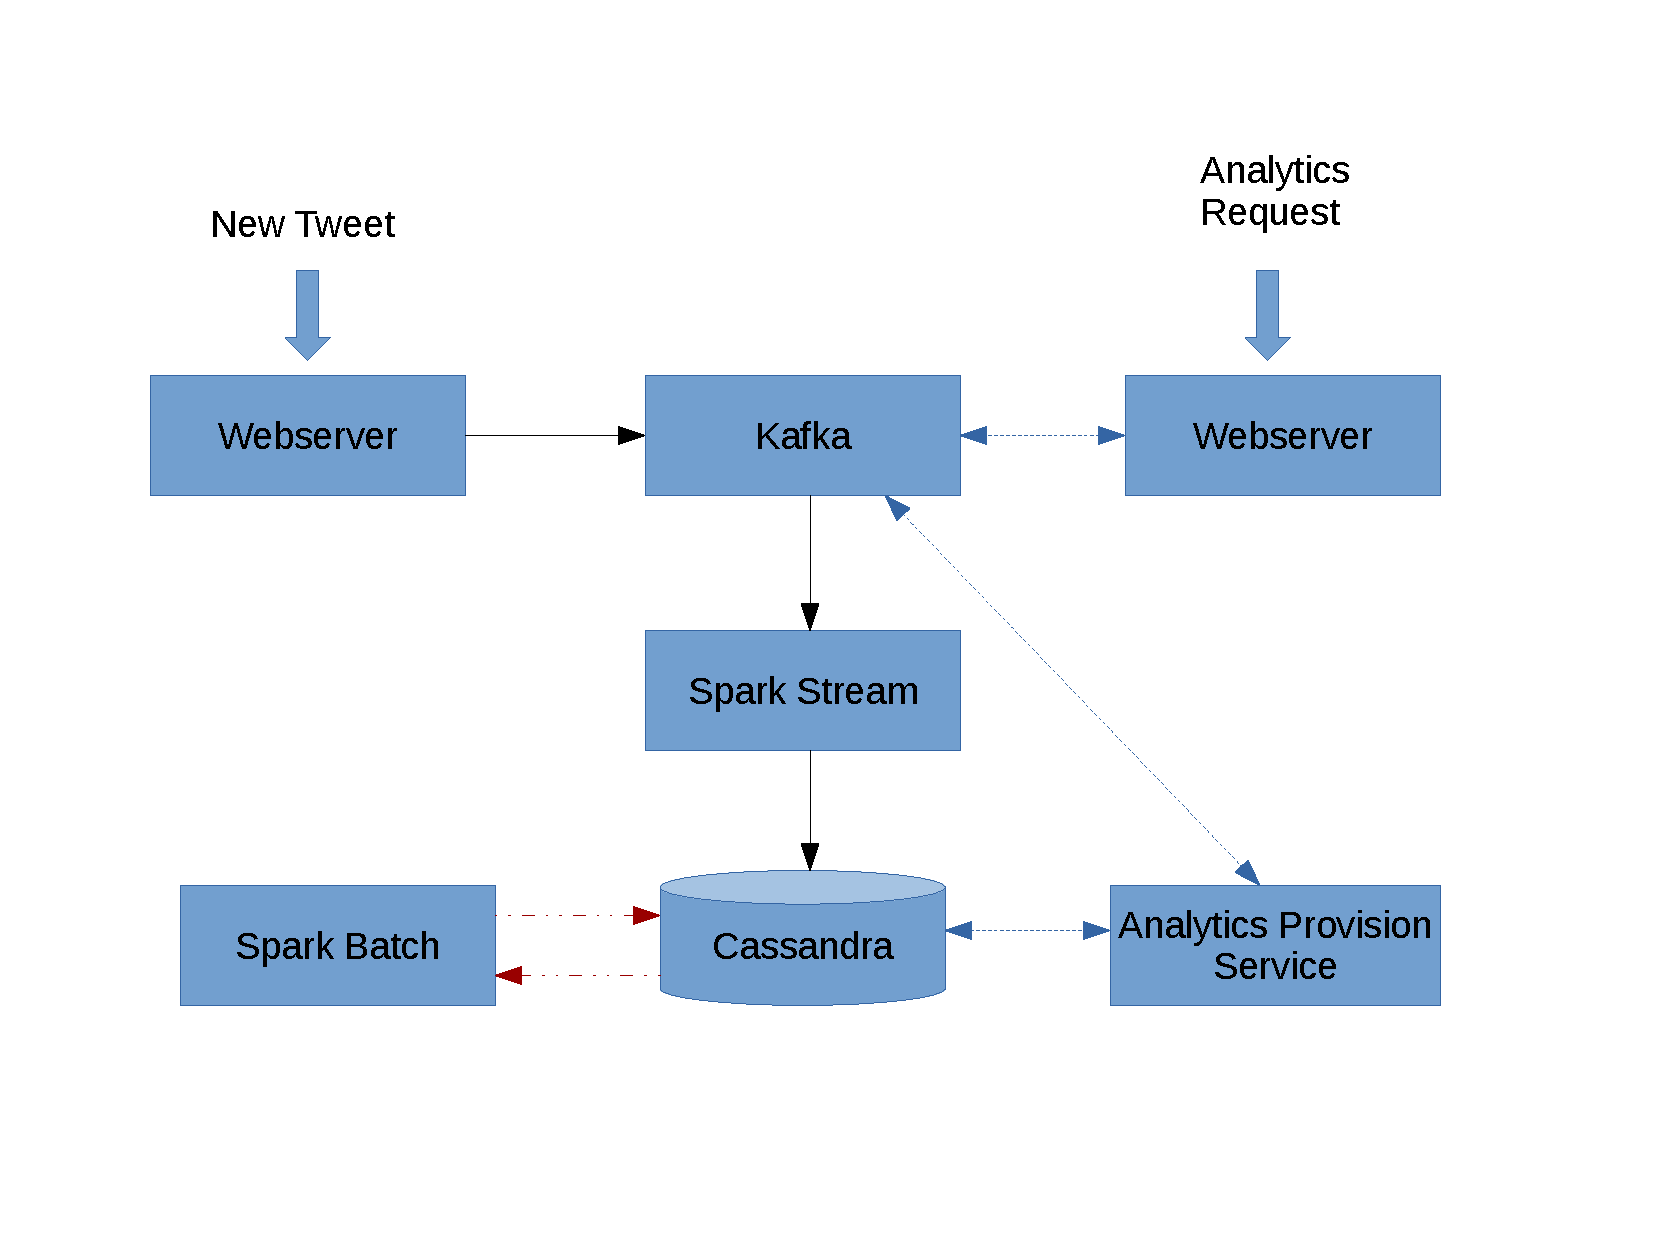
\includegraphics[width=\textwidth]{pics/analytics/archi}
	\caption{Übersicht der Analytics Komponenten}
\end{figure}

\section{Stream}

Die Streamverarbeitung innerhalb des Hamaube-Systems ist als eigenständiger Service geschrieben. Für die Umsetzung wurde SparkStreaming im Verbund mit Scala verwendet.

Folgende Ziele haben sich während des Projekt herausgebildet:
\begin{itemize}
	\item Vorverarbeitung der eingehenden Tweets für eine spätere Prozessierung mittels Spark
	\item Verarbeitung der Streamdaten für live Analyseergebnisse.
\end{itemize}


Als Input dienen bisher die beiden gegebenen Datenquellen:
\begin{enumerate}
	\item Tweets, welche aus der Twitter API in unsere Anwendung gestreamt werden.
	\item Hamaube-Tweets, welche in unserer Anwendung erzeugt werden.
\end{enumerate}

Auch die Streamverarbeitung ist über Kafka angebunden und erhält die Tweets über das \textit{USER\_ISSUES\_TWEET} Topic.


\subsection*{Vorverarbeitung für Spark Batch Processing}
Aus verschiedenen Gründen wurde für die Tweets im Hamaube-System das Datenmodell von Twitter übernommen.
Dadurch enthalten Tweets (vorallem solche, die direkt von Twitter kommen) eine Vielzahl von nicht gesetzten Feldern oder Daten, welche für die Analyse wenig interessant sind.
In der Vorverarbeitung wird nur ein definierter Teil der Felder eines Tweets übernommen und der Rest verworfen.
Zusätzlich werden (sofern vorhanden) die im Tweet enthaltenen Hashtags extrahiert und neben dem eigentlichen Tweet gespeichert.
Außerdem wird anhand des Tweet-Textes eine Sentiment Analyse durchgeführt, welche dem Tweet einen Score zuordnet, der dessen Stimmung wiederspiegelt (negativ - negative Stimmung, positiv - positive Stimmung). Auch dieser Score wird neben dem eigentlichen Tweet gespeichert.

Wir haben uns dazu entschieden, die Tweetdaten zusätzlich - also dupliziert - zu den schon gespeicherten Tweets des 'CassandraReaders' in Cassandra zu speichern, da wir in Hinsicht auf ein produktives System die kritischen Tabellen nicht zusätzlich mit Anfragen belasten wollen.
Für die Analyse würde also ein separate Umgebung für Cassandra aufgebaut, dies haben im Hamaube-System aufgrund der Einfachheit noch nicht umgesetzt.

\subsection*{Live Analyse}
Zudem wird auf den durch Kafka eingehenden Tweetstream eine Live Analyse durchgeführt.
Das Spark Streaming Framework teilt den Stream dafür in Micro-Batches, die dann weiter verarbeitet werden können.
So werden z.B. die Anzahl von Hashtag pro Stunde/pro Minute ermittelt, daraus werden dann aktuell beliebte Hashtags erkannt.
Auch diese Ergebnisse werden in Cassandra gespeichert.
Um eine Skalierungs zu ermöglichen müssen die Ergebnisse z.B. pro Stunde von mehreren Instanzen geupdated werden können, ohne dass dabei dirty reads oder Überschreibungen auftreten dürfen. Cassandra bietet hier den Datentyp \textbf{Counter}, der atomare \textit{increase} und \textit{decrease} Operationen anbietet. Damit lassen sich die meisten Szenarien realisieren, ohne weitere  komplexe (und möglicherweise verlangsamende) Isolierungsmechaniken zu implementieren.
\begin{figure}[htbp!]
\centering
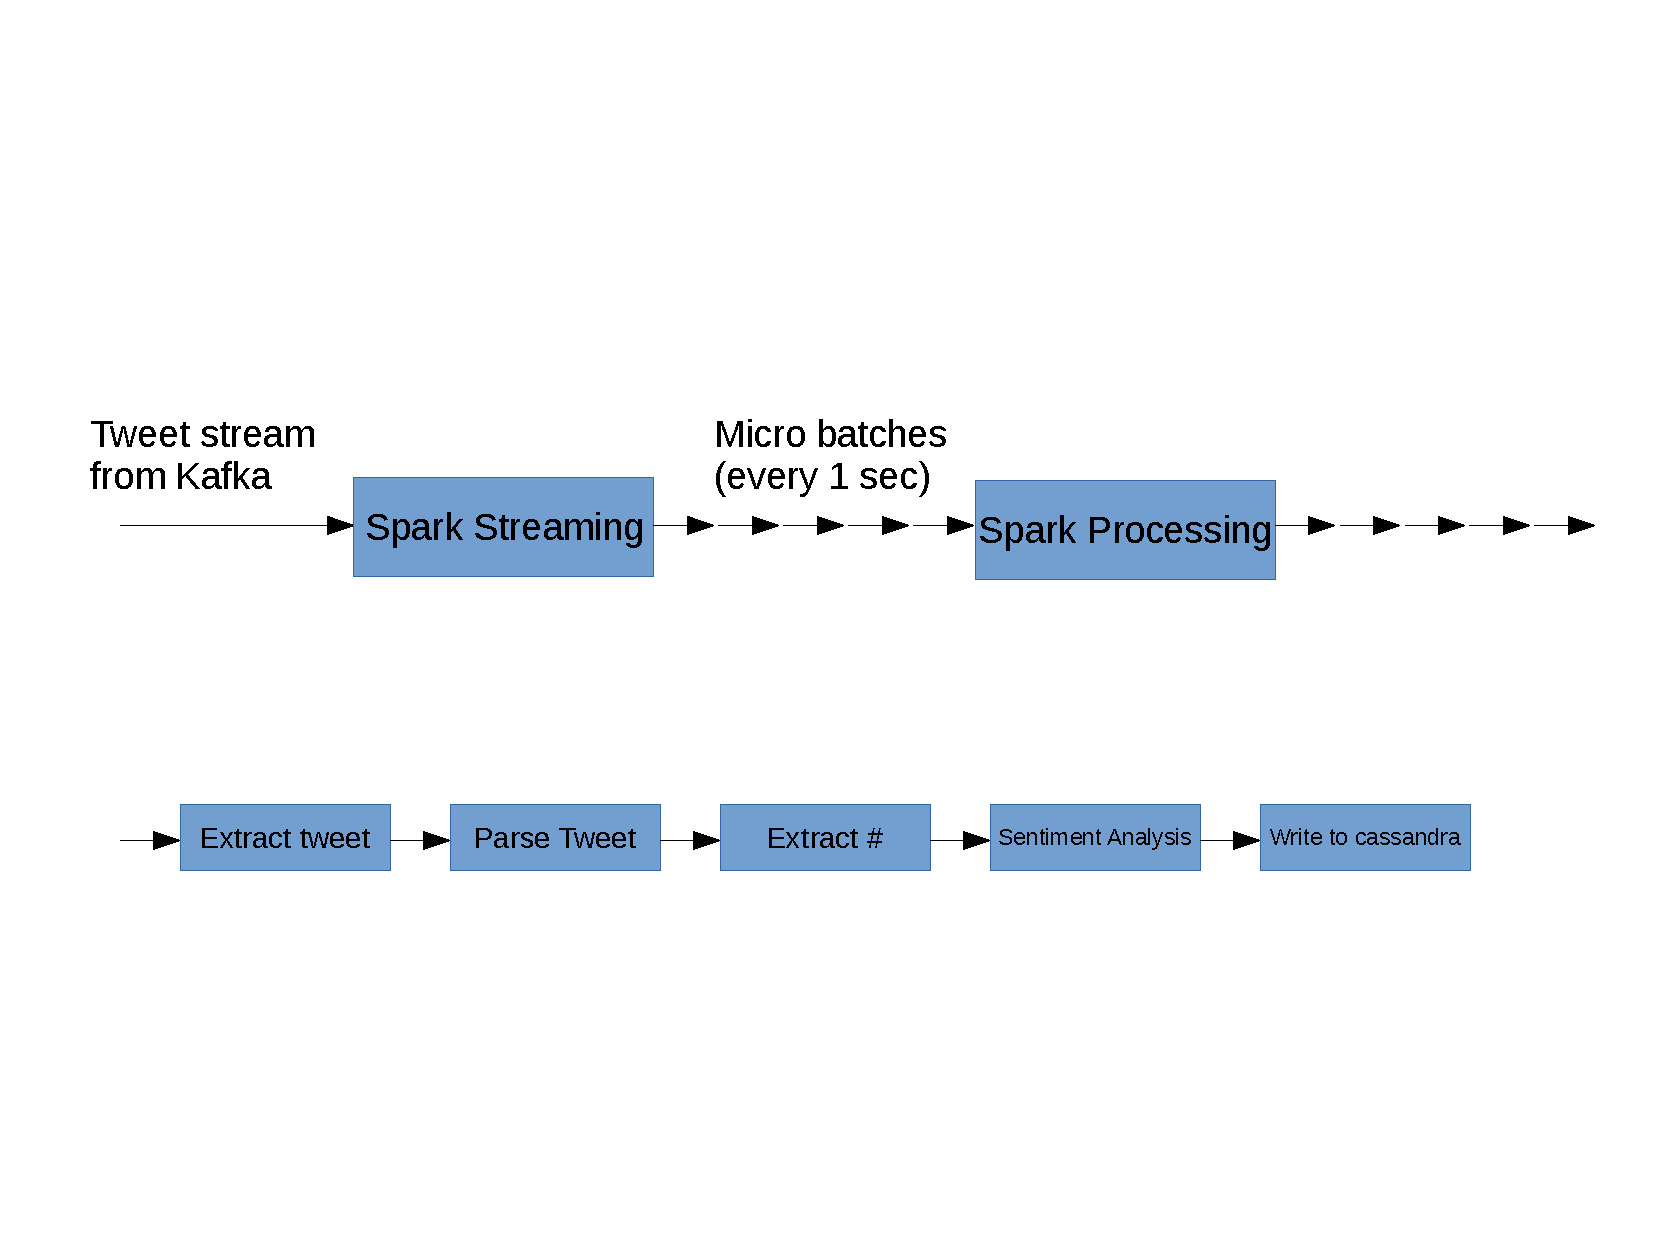
\includegraphics[width=\linewidth]{pics/analytics/streamProcessing.pdf}
\caption{Spark stream processing}
\label{fig:streamProcessing}
\end{figure}

....
% This file was converted to LaTeX by Writer2LaTeX ver. 1.0.2
% see http://writer2latex.sourceforge.net for more info
\documentclass{article}
\usepackage[utf8]{inputenc}
\usepackage[T1]{fontenc}
\usepackage[ngerman]{babel}
\usepackage{amsmath}
\usepackage{amssymb,amsfonts,textcomp}
\usepackage{array}
\usepackage{listings}
\usepackage{hhline}
\usepackage[pdftex]{graphicx}
\author{}
\date{2018-10-07T22:20:48.763142593}
\begin{document}
\section[Architektur]{\selectlanguage{ngerman} Architektur}
\subsection[zwei Phasen]{\selectlanguage{ngerman} zwei Phasen}
Die Ausführung der Analysen erfolgt in zwei Phasen. Die eine Phase ist
die eigentliche Batch-Analyse. Dabei werden alle bisher in der
Datenbank befindliche Tweets ausgewertet. Die andere Phase erfolgt
davor. Die Realtime-Analytics-Komponente überträgt die reinkommenden
Tweets in einer Art ETL-Prozess (extract, transform, load) in die
Datenbank. Dort werden sie in einem für die Analyse optimierten Format
gespeichert.

\subsubsection[ETL{}-Prozess]{\selectlanguage{ngerman} ETL-Prozess}
Der ETL-Prozess wurde ursprünglich notwendig, weil der
Cassandra-Connector für Spark einen Bug enthielt. Befanden sich an
speziellen Stellen im orginalen JSON-Objekt von Twitter NULL-Werte und
wurden diese in die Datenbank geschrieben, dann konnte der Connector
diese Objekte nicht korrekt verarbeiten. Die Tweets aus der Datenbank
werden auf ein Java-Objekt gemappt. Dabei wird versucht, alle Attribute
der Zielklasse mit Werten zu belegen. Dafür wird in der Datenbank nach
einer geeigneten, d.h. exakt gleich benannten Spalte gesucht. Dann wird
abhängig vom Datentyp der Spalte der gelesene Wert in den
entsprechenden Java-Typ umgewandelt. Der Bug tritt nun in der
Verschachtelung auf. Die JSON-Objekte können verschachtelt werden und
ebenso die Datenbank-Spalten. Dafür kann man zuerst den Datenbanktyp
selbst definieren und dann kann dieser als so genannter frozen-type
\ als normaler Spaltentyp genutzt werden. Wenn ein solches Objekt eines
frozen-types nun in der Datenbank als NULL abgespeichert ist, stolpert
der Connector darüber und findet keinen Umwandler von NULL zu einem
entsprechenden Java-Objekt.

Wir haben dann vom direkten Lesen der Tweets aus dem Datenbankteil, in
dem der Webserver sie schreibt, auf Lesen der Tweets aus einem eigenen
Datenbankteil umgestellt. Die Tweets kommen über Kafka an den
Realtime-Analytics-Prozess, der diese auswertet (extract). Der
zugehörige Kafka-Connector enthält keinen solchen Bug.

Vor dem Laden in die Datenbank wird der Tweet nun stark reduziert, d.h.
es werden viele Felder entfernt, die für die Analyse gar nicht benötigt
werden. Zudem werden die NULL-Werte an den kritischen Stellen durch
Dummy-Objekte ersetzt (transform). Schlussendlich werden sie vom selben
Cassandra-Connector in die Datenbank geschrieben, mit dem sie später
auch gelesen werden. (load).

Neben der nun vorhandenen Kompatibilität mit dem Cassandra-Connector
führt der ETL-Prozess auch zu deutlich kleineren Tweet-Objekten, was
die Analyse stark beschleunigt, insbesondere wenn die Tweets über das
Netzwerk übergeben werden müssen.

\subsubsection[eigentliche Analyse]{\selectlanguage{ngerman} eigentliche
Analyse}
Nach dem ETL-Prozess kommt die eigentliche Analyse. Der ETL-Prozess wird
ständig von der Streaming-Komponente ausgeführt, d.h. es werden Tweets
sekündlich in die Datenbank geladen.

Die eigentliche Analyse, eine Batch-Analyse wird regelmäßig, z.B. nachts
durchgeführt. Sie dauert auch deutlich länger, sie könnte gar nicht in
Echtzeit erfolgen. Ziel der eigentlichen Analyse ist es, statistische
Werte über die Aktivität der User und Inhalte der Tweets zu ermitteln.
Hierbei geht es um die Gesamtheit der Tweets. Desweiteren werden
weitere Parameter ermittelt und Empfehlungen vorbereitet. Diese
beziehen sich auf einzelne Tweets bzw. User.

\section[Skalierbarkeit]{\selectlanguage{ngerman} Skalierbarkeit}
Übergeordnetes Ziel dieses Projektes ist ja die Implementierung in einer
skalierbaren und erweiterbaren Architektur. Das Prinzip dafür lautet:
nutze skalierbare Komponenten und verbinde sie skalierbar. Mit
skalierbar ist hier scale-out gemeint, d.h. die Daten aus der Datenbank
liegen auf verschiedenen Servern vor. Die Datenbank kümmert sich um die
Verteilung der ihr zugeführten Daten. Cassandra skaliert durch die
Verteilung der Daten auf verschiedene Server. Ähnlich skaliert Spark.
Spark wird ebenso auf verschiedenen Rechner ausgeführt, die zusammen
als Cluster die Analyse ausführen. Dabei werden die Daten auf dem
Rechner gehalten, der auch die Analyse durchführt. So weit, so gut.
Allerdings gibt es hier nun einen Stolperstein, der die Skalierbarkeit
gefährdet. Die Daten liegen bisher in Cassandra und müssen zu den
Spark-Rechnern übertragen werden. Hier gibt es nun drei denkbare Wege:

\begin{itemize}
\item die Daten werden von einem Koordinator aus Cassandra abgerufen und
in Sparks verteiltes Dateisystem geladen. Offensichtlich ist dieser
Koordinator ein Flaschenhals. Dieser Fall sollte dementsprechend
vermieden werden, erfordert aber einen eigenen Sparkconnector zu
Cassandra.
\item die Daten werden von den einzelnen Spark-Rechner passend
abgerufen, d.h. jeder Spark-Rechner ruft die für ihn notwendigen Daten
ab und die Analyse wird so verteilt, dass diese Datenmengen
untereinander überschneidungsfrei sind.
\item die Berechnung folgt den Daten. Die Analyse von Spark wird auf den
Rechner ausgeführt, auf denen auch Cassandra die Daten hält. Dann
würden sie nur auf dem Rechner übertragen. Offensichtlich würde diese
Variante besonders wenig Netzwerktraffic generieren. Allerdings würde
die Rechnenlast auf den Cassandra-Knoten steigern. Wenn diese Knoten
nun auch die Produktiv-Knoten für die Datenbank des Frontends wären,
müsste man diese Effekte abwägen. Hat man allerdings eine eigene
Datenbank bzw. einen eigenen Keyspace für die Analysen, so müsste man
diese Effekte nicht gegeneinander abwägen. Und wir haben ja einen
solchen Keyspace für die Analysen, der mit dem ETL-Prozess gefüllt wird.
\end{itemize}
Wir verwenden einen Cassandra-Connector in Spark, der das letzte Prinzip
versucht. Er versucht die Analysen möglichst auf dem gleichen Knoten
auszuführen, auf dem auch die Daten in Cassandra liegen. Möglich wird
dies dadurch, dass man diese Informationen aus Cassandra abrufen kann
und dass Spark die Möglichkeit bietet, die Verteilung der Analysen
genau aus solchen Gründen zu beeinflussen. In unserem Testsetup
funktioniert das leider nicht, da keine gesonderten Knoten für die
Analytics-Cassandra-Instanz zur Verfügung stehen und Spark auf anderen
Knoten läuft. Damit entspricht unsere skalierbare Verbindung der aus
dem zweiten Fall.

Der dritte Fall, auch genannt Datenlokalität, ist nicht unbedingt der
bessere. Nicht nur, wenn die Datenbankknoten noch mit anderen Dingen
beschäftigt sind, nein auch, wenn die Analyse im Vergleich zum Laden
der Daten komplexer wird, also mehr Rechenleistung benötigt wird.
Ausprobiert wurde deshalb auch, wie sich unsere Analysen verhalten,
wenn man sie zwar auf mehr CPU-Kernen ausführt, dafür aber ein
langsameres Netzwerk simuliert. Die Anzahl parallel laufender Einheiten
ist deutlich sichtbar. Es werden so viele Einheiten gleichzeitig
fertig, wie der Prozessor Kerne hat. In diesem Fall zeigt aber eine
Auswertung der CPU-Last, dass die Übertragung über das Netzwerk der
Flaschenhals ist, denn die CPU-Kerne sind max. zu Hälfte ausgelastet.
Ist das Netzwerk schneller, dann steigt auch die CPU-Auslastung auf
nahezu 100\%.

\subsubsection[mit Flaschenhals]{\selectlanguage{ngerman} mit
Flaschenhals}

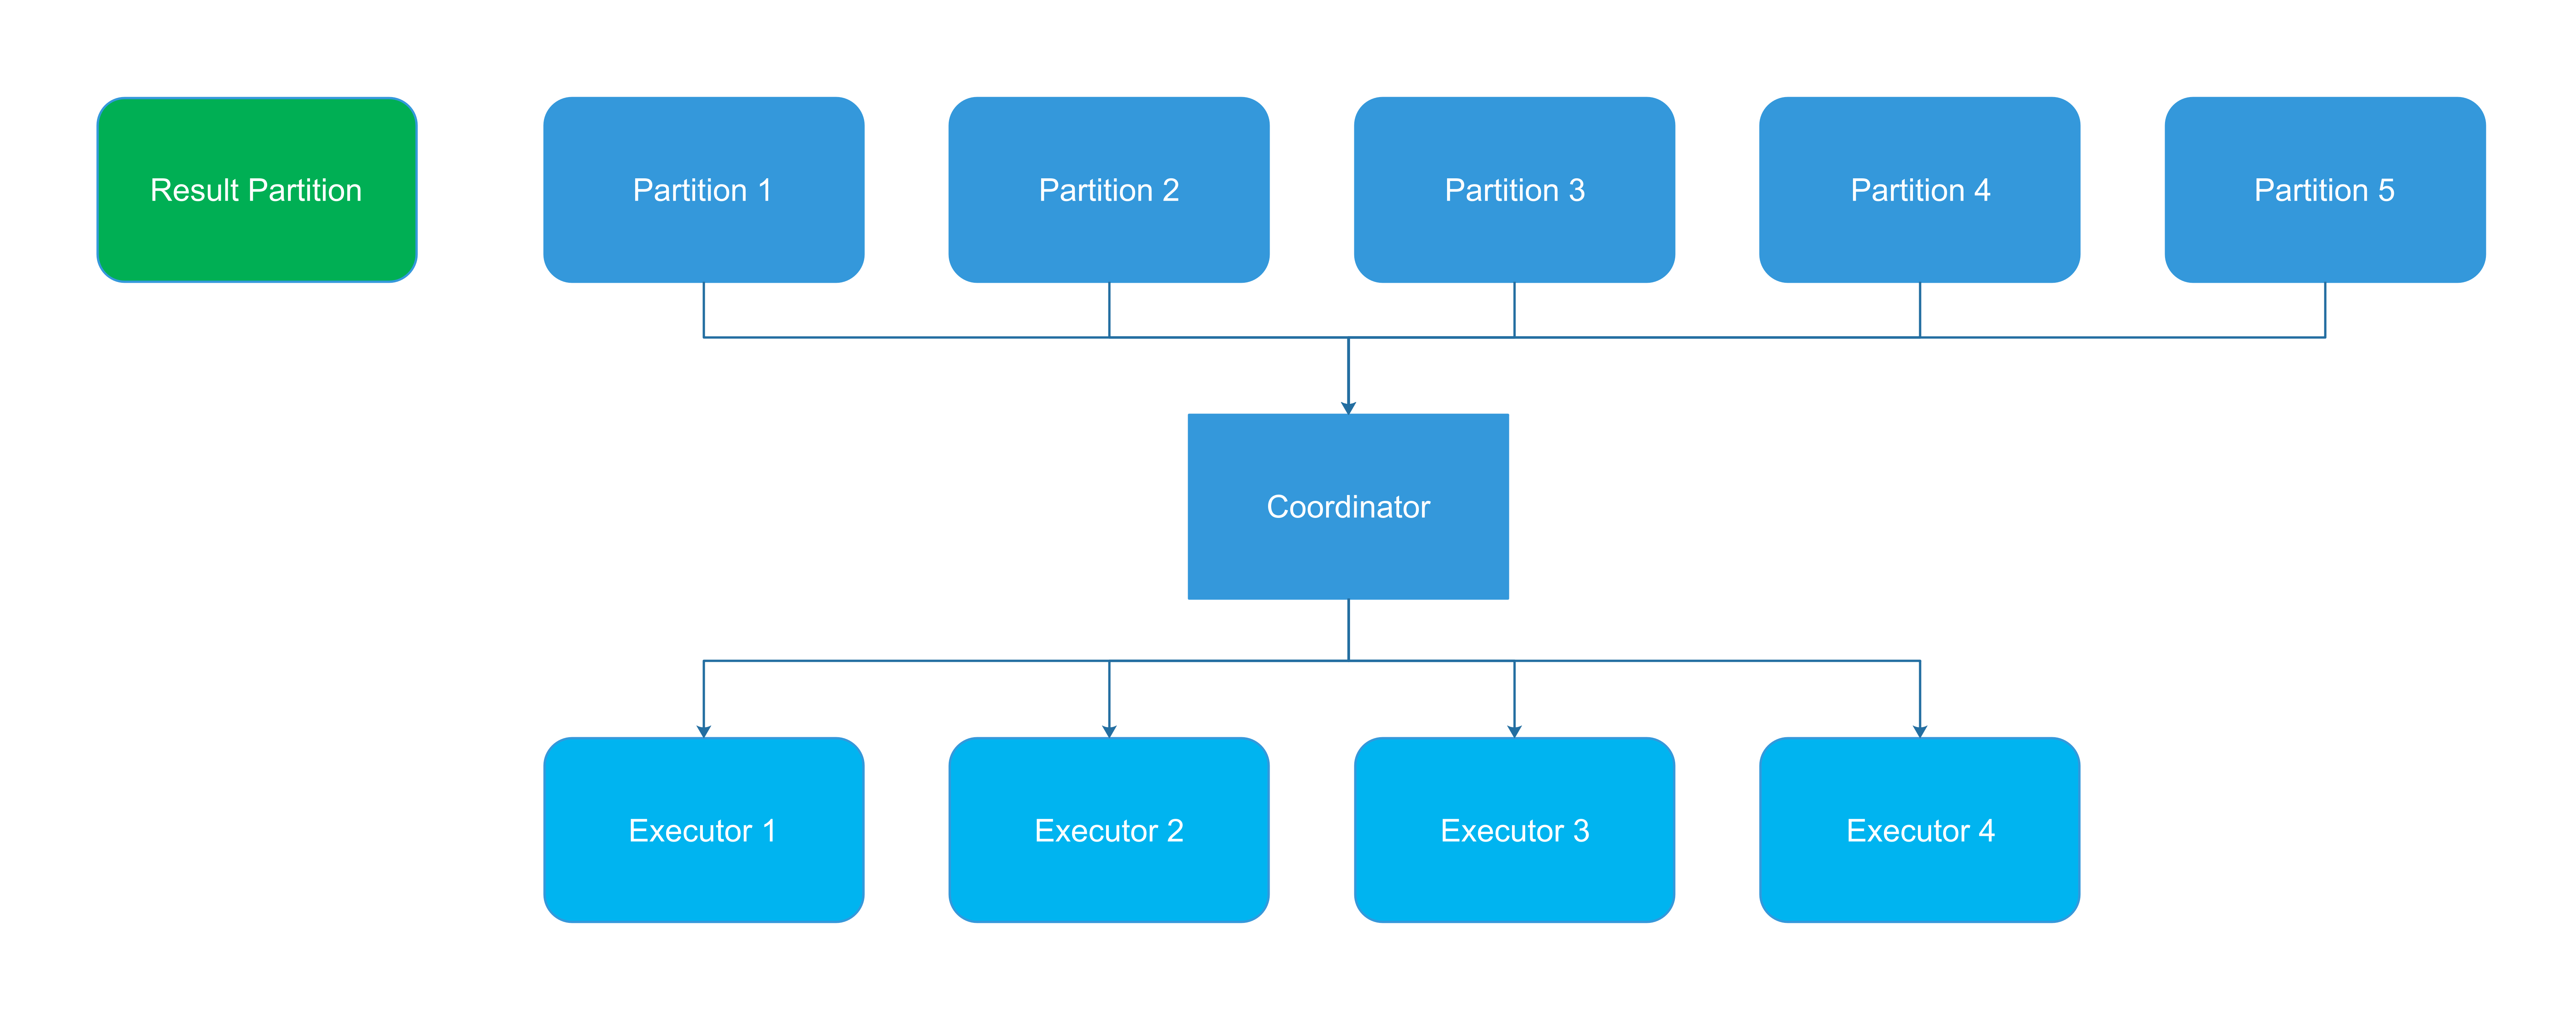
\includegraphics[width=15.24cm,height=5.99cm]{bilder/eigene20PrC3A4sentation-img1.png}


\subsubsection[Durcheinander]{\selectlanguage{ngerman} Durcheinander}

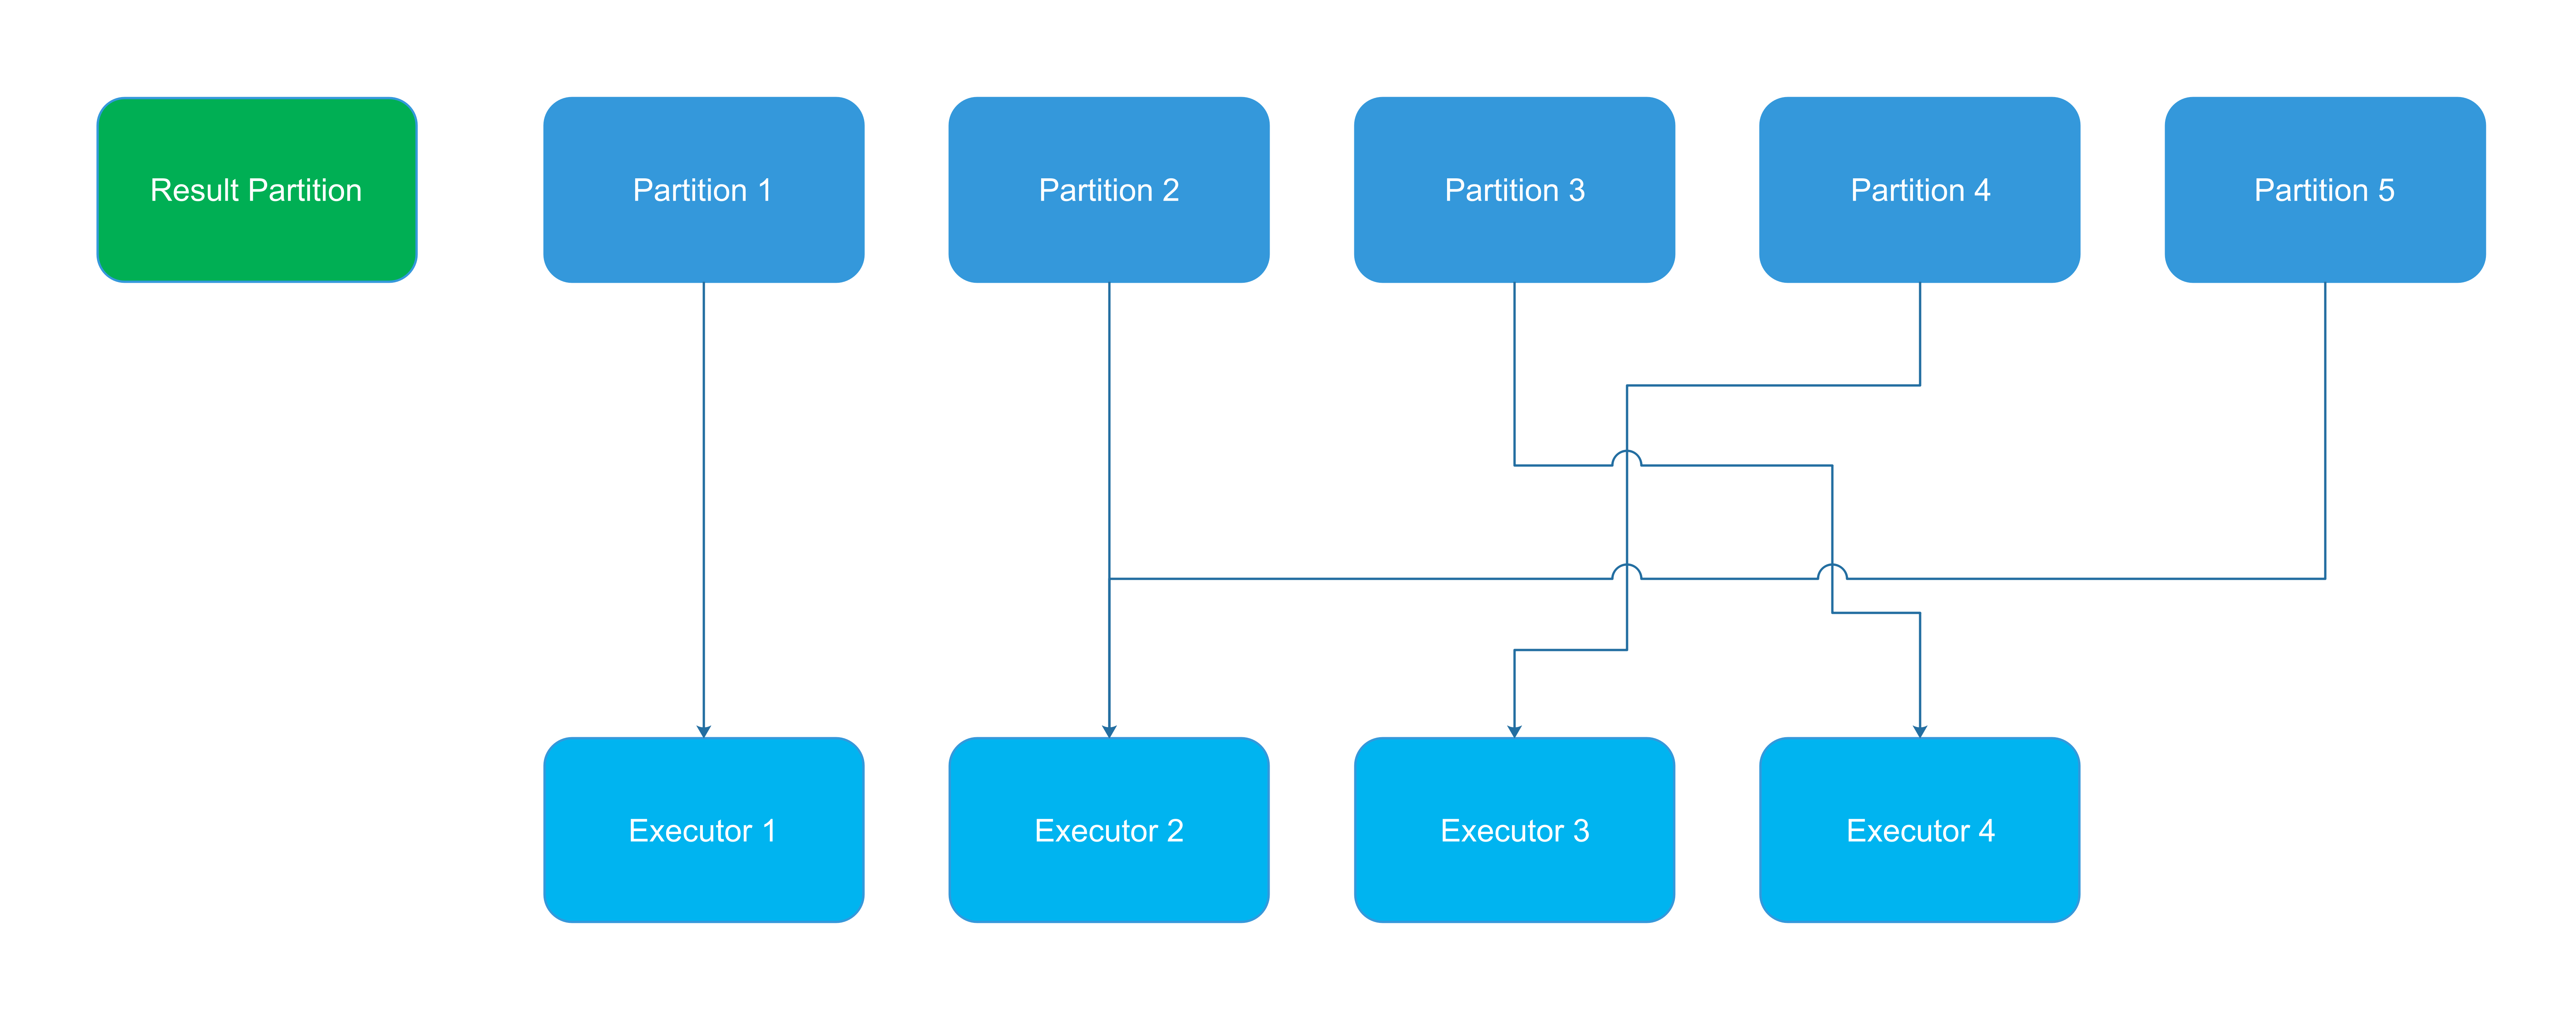
\includegraphics[width=15.24cm,height=5.99cm]{bilder/eigene20PrC3A4sentation-img2.png}


\subsubsection[mit Data Locality]{\selectlanguage{ngerman} mit Data
Locality}

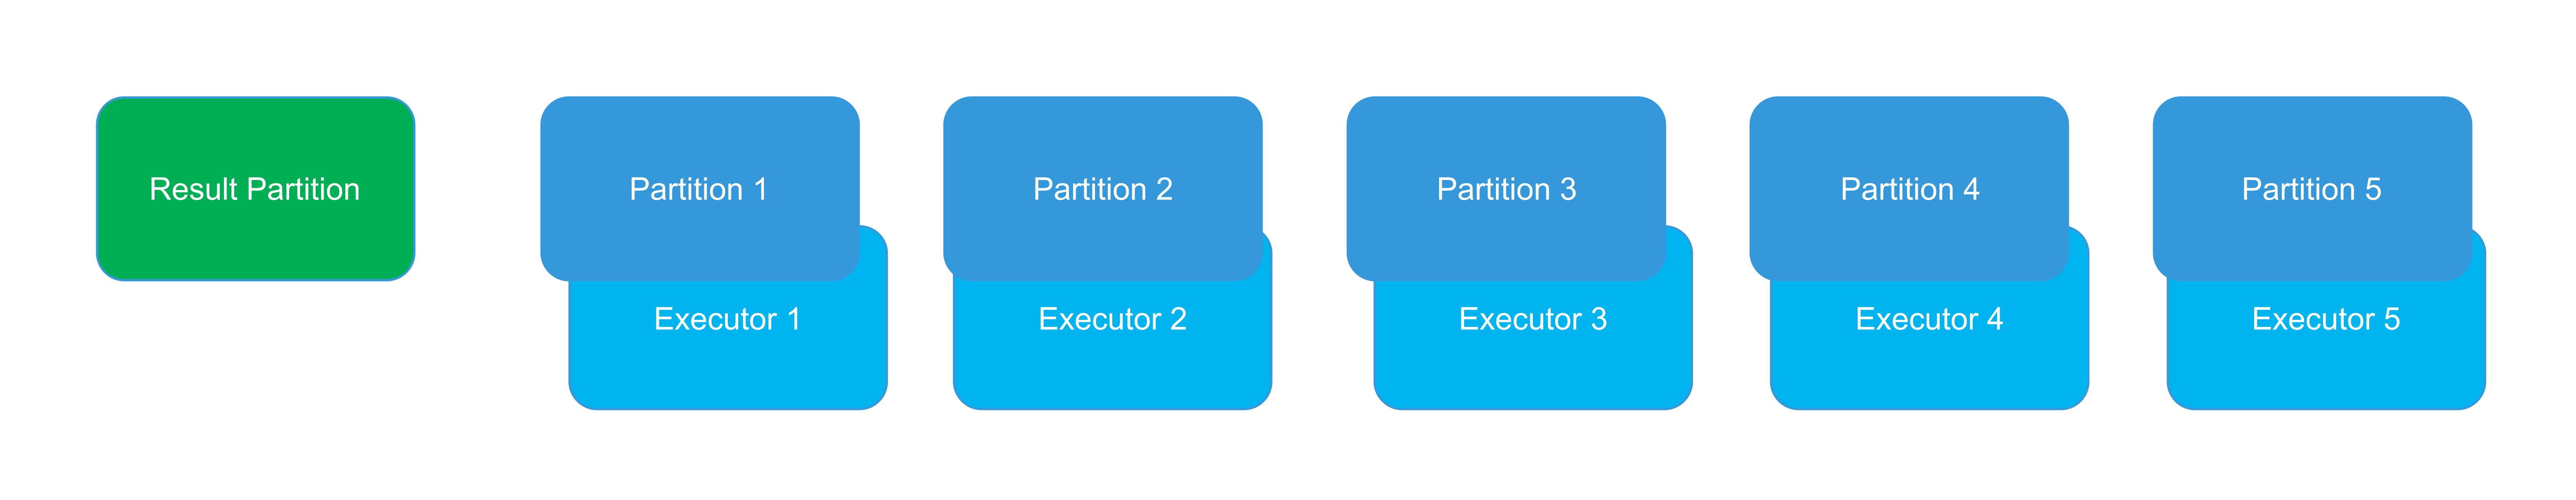
\includegraphics[width=15.24cm,height=2.956cm]{bilder/eigene20PrC3A4sentation-img3.png}


\section[Use{}-Cases]{\selectlanguage{ngerman} Use-Cases}
Die Batch-Analytics-Komponente hat vorrangig das Ziel, inhaltlich
relevante Entwicklungen in den Tweets zu zeigen. Das wären z.B. länger
trendende Hashtags zu identifizieren.

Folgende statistische Werte werden erhoben und im Frontend angezeigt:

\begin{itemize}
\item Gesamtanzahl Tweets
\item Anzahl fröhlicher Tweets (gemessen am Vorliegen eines Smileys) und
Anzahl trauriger Tweets (Vorliegen eines Sadleys)
\item \ die Anzahl Tweets pro Tag
\item \ die Top 10 Hashtags pro Tag
\item \ die Top 10 Stunden mit dem meisten Tweets pro Tag
\item \ die Top10 Tweeter pro Tag
\item sowie die Top 10 verwendeten Wörter pro Tag.
\end{itemize}
Eine Vorstellung der Ergebnisse findet sich weiter unten.

Diese Daten werden von Spark ermittelt und in eine Ergebnistabelle von
Cassandra geschrieben. Dort werden sie vom AnalyticsServices bei
Anfrage durch den Webserver ausgelesen und an den Webserver gesendet.
Dieser wiederum leitet sie an das Frontend weiter, wo sie mittels
Javascript grafisch dargestellt werden.

Weiterhin sind folgende Anwendungen in Spark implementiert:

\begin{itemize}
\item Analyse der Tweetsprache durch Analyse der vorkommenden
Stopwords
\item Ermittlung von zeitlichen Aktivitätsprofilen der User
\item Ermittlung von Association-Rules für das Folgen von Nutzern.
\end{itemize}
Die erste beiden Komponenten werden im Frontend nicht aktiv eingesetzt.
Die letzte Komponente kann nicht sinnvoll benutzt werden, da im
Gegensatz zu den vielen Tweets unsere Userdaten sehr lückenhaft sind.
Es fehlen die Informationen über die gefolgten Nutzern bzw. nur ein
Nutzer in unserer Datenbank hatte mehr als einen Follower. Damit ließen
sich keine Association-Rules generieren. Der einzige Nutzer, dem mehr
als ein Nutzer folgt (zwei Nutzer) ist der Twitter-Account der
übermäßig präsenten koreanischen Boyband BTS. Sie wird später nochmal
genauer angeschaut.

Ein weiterer Usecase für die grafischen Analysen ist die Überprüfung der
Funktionsweise des Systems. Werden die Daten aufgrund einer
Schema-Änderung bei Twitter nicht mehr in die Datenbank gespeichert, so
würde man dies in den Analysen sehen können. Auch ein
Programmierfehler, bei dem der Benutzername nicht richtig übertragen
wurde, fiel auf. Statt Tweetern mit ca. 40-80 Tweets pro Tag tauchte in
den Top 10 der Tweeter nur ein Nutzer auf, nämlich NULL.

Ein dritter Usecase fällt bei der Analyse der Top-Hashtags auf. Am
27.09. z.B. ist einer der Top10-Hashtag PCA. Das steht für
People{\textquotesingle}s Choice Award. Es handelt sich hierbei um eine
Online-Abstimmung, die durch Nennungen in den sozialen Medien erfolgt.
Zur Auswertung ist eine solche Gesamtanalyse natürlich nötig.

\subsection[Erkenntnisse durch grafisch aufbereite
Statistiken]{\selectlanguage{ngerman} Erkenntnisse durch grafisch
aufbereite Statistiken}
Wir haben eine einfache Sentiments-Analyse eingebaut. Ziel ist es, die
insgesamte Stimmung auf einer Skala von positiv bis negativ einordnen
zu können. Die Sentiments-Analyse wertet die Tweets auf das Vorkommen
von Smileys :-) und Sadleys :-( aus. Die jeweilige Gesamtzahl wird dann
angezeigt. Diese Methode ist offensichtlich ziemlich ungenau und das
zeigt sich auch in den Ergebnissen. Am 1.10.2018 hatten wir fast 10
Millionen Tweets in der Datenbank, aber nur 2177 enthielten ein Smiley
und sogar nur 366 ein Sadley.

Hier zeigt sich auch beispielhaft, warum eine Arbeitsteilung zwischen
Datenbank und Analysen sinnvoll sein kann. Die Datenbank kann nämlich
nicht ausgeben, wie viele Tweets in ihr speichert sind. Die
entsprechende Anfrage timed out. Für andere Anfragen ist ein geeigneter
Index notwendig. Dessen Notwendigkeit ist nicht immer im Voraus bekannt
und eine Nachrüstung kaum möglich.

\section{\selectlanguage{ngerman}
interessante Analyseergebnisse}
\subsection[BTS]{\selectlanguage{ngerman} BTS}
Bei unseren Analysen war der Hashtag BTS in verschiedenen Formen immer
präsent. BTS steht für Bangtan Boys und ist eine koreanische Boyband.
Ihre hohe Präsenz auf Twitter ist nicht nur Folge hoher Popularität und
der Auswahl durch Twitter, sondern auch Ergebnis diverser
Social-Media-Kampangen. BTS startete unter anderem die
LoveYourself-Kampange. Ziel derer ist es, die Liebe in der Welt zu
verbreiten. Aussage ist es, dass für die Liebe in der Welt zuerst die
Selbstliebe notwendig ist. Diese Jahr sprachen sie vor den Vereinten
Nationen zu diesem Thema. Ein weiterer Hashtag aus dem BTS Umfeld ist
deren A.R.M.Y, was für Adorable Representative M.C for Youth steht.
Damit wird ihr Fanclub bezeichnet.

Eine These, warum es gerade BTS so konstant in unsere Tweets schafft,
ist dass unser Selektionskriterium love diese LoveYourself-Kampange
trifft.


\includegraphics[width=15.24cm,height=8.557cm]{bilder/eigene20PrC3A4sentation-img4.png}

\bigskip

\subsection[Twitter{}-Spam]{\selectlanguage{ngerman} Twitter-Spam}
Die Analyse der Top 10 Tweeter am 23. und 24.09.2018 zeigt ein weiteres
interessantes Phänomen: den Twitter-Spam. Mit der Möglichkeit sich an
bekannte Hashtags hängen zu können, zieht Twitter auch Spammer an. Am
24.09.(und am 23.09) \ hat es eine Gruppe von Usern geschafft, durch
jeweils 30 Tweets pro Nutzer unsere Top 10 mit Porno-Spam zu füllen,
mit User wie DAILY HOMEMADE, und THE PORN PROMO LIST. In den
darauffolgenden Tagen tauchen sie dann nicht mehr auf, was für
Gegenmaßennahmen auf Seiten Twitters spricht. Am 01.10.2018 tauchen sie
dann langsam wieder in den Top 10 auf.

\subsection[Trump related]{\selectlanguage{ngerman} Trump related}
In unseren Daten sind jeden Tag große Mengen von Tweets über/mit Donald
Trump enthalten. Neben seiner bekanntermaßen hohen Twitterpräsenz liegt
das auch an dem Selektionskriterium, mit dem wir bei Twitter nach
Tweets anfragen. Es enthält unter anderem den Selektor Trump.

\section[spezielle Analyseergebnisse]{\selectlanguage{ngerman} spezielle
Analyseergebnisse}
\subsection[stream{}-bedingte Ergebnisse]{\selectlanguage{ngerman}
stream-bedingte Ergebnisse}
Es gibt einige Gründe, die unsere Analyseergebnisse verzerren.

Der erste Grund ist die konstante Geschwindigkeit unseres
Twitterstreams. Offensichtlich verarbeiten wir nicht 100\% der Tweets
weltweit oder auch nur deutschlandweit. Stattdessen lassen wir uns von
Twitter über deren API eine Auswahl geben. Die API liefert maximal 80
Tweets pro Sekunde aus. Wir haben diese Rate auf 2 Tweets pro Sekunde
limitiert. Am 24.09.2018 kommen alle
Stunden auf $7918 \pm 5$ Tweets. Das entspricht gerade
der Streamgeschwindigkeit.

Zudem lassen z.B. am 01.10 auch die Auswirkung der Analysezeit sehen. An
diesem Tag lief der Stream nur zeitweise und genau diese Zeiten lassen
sich erkennen. Er wurde irgendwo zwischen 10 und 11 Uhr angeschaltet
und lief zwischen 11 und 12 wieder vollständig (ca 7200 Tweets). Nach
12 Uhr wurde er wieder unterbrochen und ca.zwischen 14:30 und 15:40
lief er dann wieder. 

\subsubsection[Sampling verzerrt die absoluten
Zahlen]{\selectlanguage{ngerman} Sampling verzerrt die absoluten
Zahlen}
Bei manchen Analysen, z.B. Tweets pro Tag stimmen die absoluten Zahlen
nicht. Am 24.09.2018 weist die Grafik 353 Tweets aus. Wir wissen aber
durch die Auswertung über die Stunden das es ca. 172800 Tweets sein
müssten (24 Stunden x 7200 Tweets pro Stunde). Das liegt daran, das
für die Grafik ein Sampling der Tweets genommen wurde, d.h es wurde nur
ein Bruchteil analysiert. Während der Entwicklung dient das dazu, dass
die Analysen schnell ausgeführt werden können (ca. 1 Minute vs. 20
Minuten). Im Produktivbetrieb würde man dieses Sampling dann nicht mehr
vornehmen.

\section[genauere Schritte]{\selectlanguage{ngerman} genauere Schritte}
Ein großes Hindernis bei der Entwicklung und dem Betrieb der Analysen
war es, dass die Beispiele und gefundenen Howtos zu einfach sind. Im
Sinne einer gewissen Wissensweitergabe sollen hier anhand einiger
Patterns – analog zu Design Patterns – die gewonnen Erkenntnisse
weitergegeben werden. 

\subsection[doppelter Key]{\selectlanguage{ngerman} doppelter Key}
Eine Herausforderung war es, dass der Mapping-Schritt zwar ein
Key-Value-Mapping vornimmt, aber nur einen Key unterstützt. Für die
Analysen wird aber häufig ein mindestens doppelter Key benötigt. Zum
Beispiel wenn die Top 10 Tweeter pro Tag bestimmt werden sollen. Dann
sieht ein typisches Key-Value-Paar eigentlich so aus (Tag, Tweeter →
1). Die beiden Angaben für den Key lassen sich einfach aus den Tweets
extrahieren. Nun müssen sie noch verbunden werden. Die einfachste
Möglichkeit, die funktioniert hat, ist die beiden Angaben jeweils in
einen String zu exportieren und die beiden Strings zu konkatenieren.
Damit die beiden Teile später wieder getrennt werden können, muss noch
ein eindeutiges Trennzeigen eingefügt werden. Kein einzelnes Zeichen
kann dafür verwendet werden, da sie alle potentiell in den Tweets
vorkommen können. Wir verwenden deshalb eine lange, zufällige
Zeichenkette, wie sie so wohl kaum in einem Tweet vorkommen wird.

Eine weitere Methode wäre es, eine eigene Klasse für das Key-Value-Paar
zu erstellen. Hierbei ist darauf zu achten, sowohl equals() als auch
hashCode() korrekt zu implementieren.

Eine dritte Möglichkeit wäre es, das in Scale eingebaute Tuple2 zu
verwenden.

Keine Möglichkeit war es, bereits zu Anfang die Daten aufzuteilen und
zuerst nach Tagen zu filtern und dann 14 Analysen laufen zu lassen. Das
würde zu lange dauern, da Spark die Daten dann zu häufig anfordern
würde (nämlich neu für jeden Tag).

Auch deshalb wäre eine bessere Unterstützung durch Spark hier sinnvoll.
Denn es gibt einen weiteren Fall, der ganz ähnlich ist.

\subsection[Top10 pro Tag nehmen]{\selectlanguage{ngerman} Top10 pro Tag
nehmen}
Unsere Analysen sind häufig pro Tag. Das bedeutet, dass wir die Top 10
für die letzten 14 Tage zum Beispiel nehmen wollen. Wir brauchen also
14 Top 10s. Die eingebaute Sortierung kann einem hier nur teilweise
helfen. Sortiert man wie normal nach Values, so ist nicht garantiert,
dass sich die Top 10 der 14 Tagen überhaupt am Anfang findet. Werden an
einem Tag besonders viele Tweets abgesendet, so verdeckt das natürlich
die anderen Tage. Die sortierte Liste enthält dann viele Einträge
der aktiveren Tage und die Top 10 der weniger aktiven Tage findet sich
weiter hinten.

Die einzige korrekte Lösung, die wir gefunden haben, ist es sich die
gesammte Liste nach dem Reduce auf einem Knoten zusammenführen zu
lassen und sie dann von oben nach unten zu iterieren. Bei der Iteration
übertragen wir das gesichtete Element die Top10 des entsprechenden
Tages, so lange der Tag nicht schon 10 Einträge in der Liste hat.

Dieses Verfahren ist allerdings unnötig wenig parallelisiert. Würde man
die Daten früh nach Tagen shuffeln, so könnte man diese Operationen
zumindest nach Tagen parallelisiert auf unterschiedlichen Knoten
ablaufen lassen.

Wahrscheinlich gibt es dafür eine Lösung in Spark. Eine einfache
Unterstützung für die Unterteilung von Daten in einzelne Klassen und
dann Durchführung der selben Operation für alle Klassen separat wäre
trotzdem sehr hilfreich. \ 

\subsection{\selectlanguage{ngerman} Bausteine}
Man sagt, dass Spark mit dem Map-Reduce-Paradigmum verwendet wird. Die
Daten werden eingelesen und auf ein Ergebnis oder einen Fall gemappt
und diese dann aggregiert (reduce). Während der Arbeit an den
Batch-Analytics wurde deutlich, dass etwas mehr Schritte vorgenommen
werden müssen. Konkret fielen die Schritte:

\begin{itemize}
\item Daten laden
\end{itemize}
Die Grundoperation für das Laden der Daten ist beim verwendeten
Cassandra-Connector der Table-Scan. Komplexere Abfragen lassen sich
(noch) nicht ausführen. Damit kann keine Selektion nach einem Kriterium
erfolgen (zum Beispiel Tweets der letzten vierzehn Tage). Diese
Selektion muss dann im Filter-Schritt erfolgen.

\begin{itemize}
\item ggf. samplen
\end{itemize}
Gerade während der Entwicklungszeit ist es ratsam, darüber nachzudenken
zuerst die Analysen mit einem (sehr) kleinen Ausschnitt der Daten
durchzuführen. Dafür kann das entstandene RDD entweder gesampelt werden
oder n Elemente davon genommen werden (take). Das erste Fall ist durch den
Salt für den Pseudo-Zufallsgenerator deterministisch, das zweite nicht.
Das erste dauert ähnlich lange wie das Laden der ganzen Daten,
insbesondere ist es unabhängig von dem Anteil der zu holenden Daten. Das
zweite, das Taken, erfolgt viel schneller. Hier werden keine weiteren
Daten mehr übertragen, sobald die gewünschte Anzahl erreicht ist. Die
Daten könnten aber weniger stark durchmischt sein.

Da unsere Operationen nicht besonders teuer sind, hat das Samplen kaum
einen Geschwindigkeitsvorteil gebracht. Für das reine Testen der
Funktionalität konnte das Taken aber mit hohem Geschwindigkeitsvorteil
eingesetzt werden.

\begin{itemize}
\item \ Filtern
\end{itemize}
Dieser Schritt ist deshalb nötig, weil die Grundoperation der Table-Scan
ist. Es können aber auch unnötige Tweets aussortiert werden, z.B.
Tweets, die nicht zu einem gewissen Thema gehören.

\begin{itemize}
\item Mappen
\end{itemize}
Der bekannte Map-Schritt. Häufig werden mehrere Eigenschaften der
Gesamtheit untersucht. Das lässt sich dadurch bewerkstelligen, dass man
ein Vektorobjekt mit Feldern für alle untersuchten Eigenschaften anlegt
und für diese separat die Werte berechnet.

\begin{itemize}
\item Reducen
\end{itemize}
Der bekannte Reduce-Schritt. Hat man während des Mappen-Schritts ein
Vektorobjekt angelegt, so muss man hier auch wieder eine Vektorreduktion
vornehmen.

\begin{itemize}
\item Ergebnis produzieren
\end{itemize}
Nach dem Reduce liegen noch ggf. viele Daten vor. Bei der Analyse der
Top Hashtags liegen z.B. zu allen überhaupt vorkommenden Hashtags die
Häufigkeiten vor. Diese müssen jetzt noch weiterverarbeitet werden, indem
 z.B. die gewünschten Daten extrahiert werden (Top 10 der letzten
vierzehn Tage).

\begin{itemize}
\item und Ergebnis abspeichern
\end{itemize}
Die Daten müssen noch zum Zwecke der Persistenz in Cassandra geschrieben
werden.

auf.


\bigskip

\section[Verbesserungsvorschläge]{\selectlanguage{ngerman}
Verbesserungsvorschläge}
Bei der Arbeit an der Spark-Komponente sind einige
Verbesserungsvorschläge aufgekommen. Man sieht deutlich, dass es sich
bei Spark und Cassandra noch nicht um jahrzehntelang erprobte und
verfeinerte Tools handelt.


\bigskip

\subsection[Frühere Fehlererkennung]{\selectlanguage{ngerman} Frühere
Fehlererkennung}
Ein tolles Feature wäre eine frühere Fehlererkennung. Bisher fallen
gerade Flüchtigkeitsfehler erst bei der Ausführung auf. Das betrifft
vor allem die zusätzlichen Aufgaben, die durch Spark und die Datenbank
hinzukommen. Beispielsweise müssen alle Datenklassen Serializable
implementieren. Meist reicht es, den Zusatz implements Serializable
hinzuzufügen. Vergisst man das, so merkt man erst bei der Ausführung
der Analyse. Ein weiteres Beispiel betrifft das Mapping zur Datenbank.
Vertippt man sich hier z.B. beim Spaltenname, so merkt man das erst bei
der Ausführung. Eine zusätzliche, automatische Analyse vor oder nach
dem Kompilieren wäre sehr hilfreich. Gerade das lange Packen (90
Sekunden) könnte so wegfallen. Sie könnte z.B. die Datenbank bereits
kontaktieren und das Mapping ausprobieren oder durch statische
Codeanalyse Fehler wie die fehlende Serializability finden.

\subsection[inkrementelles Packing]{\selectlanguage{ngerman}
inkrementelles Packing}
Eine andere Verbesserung wäre das inkrementelle Packen. Ändert man einen
kleinen Fehler in einer Klasse wird die Fat-Jar mit allen
Abhängigkeiten erneut gebaut. Allerdings würde der Austausch der
veränderten Klassen ausreichen. Wenn ein solches inkrementelles Packen
möglich wäre, dann würde dies eine große Unannehmlichkeit beheben. In
der Scala-Variante scheint dies zu erfolgen, hier braucht das Packen
nicht so lange.

\subsection{automatisches Zusammenlegen von
Analysen}
Die dritte Verbesserung betrifft die Ausführung mehreren Analysen. In
unserem Fall werden sehr ähnliche Analysen auf den gleichen Daten
ausgeführt. Das Laden der Daten aus der Datenbank dauert allerdings
verhältnismäßig am längsten. Hier wäre es zu begrüßen, wenn die
Analysen automatisch zusammengelegt werden können. Gerne kann man das
auch im Code explizit aktivieren müssen.

Ein Beispiel ist das Zählen von Smileys und Sadleys. Dies könnte ohne
Problem gleichzeitg erfolgen. Es ist nicht erforderlich, zuerst alle
Daten aus der Datenbank zu holen und die Smileys zu zählen und dann
wieder alle Daten aus der Datenbank zu holen und jetzt die Sadleys zu
zählen.

Natürlich lässt sich das auch manuell im Code machen, indem man einen
Analysevektor für die Values erzeugt. Das macht aber die Kopplung im
Code wieder höher und macht z.B. beim Sortieren Probleme, da eigene
Comperatoren neu geschrieben werden müssen oder die Daten vorher wieder
zerlegt werden müssen.

Würde das automatisch erledigt werden, könnten die Analysen insgesamt
deutlich schneller werden, da die Daten nur einmal aus der Datenbank
geholt werden würden.

\section[Probleme]{\selectlanguage{ngerman} Probleme}
In diesem Abschnitt soll auf die häufigsten und/oder nervigsten Probleme
eingegangen werden.

\subsection[sehr lange Ausprobierzeiten]{\selectlanguage{ngerman} sehr
lange Ausprobierzeiten}
Bedingt durch mehrere Effekte dauert es vom Ändern des Codes bis zur
fehlerhaften oder erfolgreichen Ausführung vergleichsweise lange. Klar
lässt sich eine Analyse mit vielen Daten nicht innerhalb kürzester Zeit
ausführen, trotzdem gibt es einige Punkte, die unnötige Wartezeiten zur
Folge haben:

Das Packen der Jar nach dem Kompilieren dauert jeweils 1:30 Minute

Unabhängig davon, wie viel Code geändert wurde, ist das zu lange. Die
resultierte Fat-Jar ist über 170 Megabyte groß. Deshalb spricht viel
dafür, dass zu viele unnötige Abhängigkeiten mitgepackt werden und/oder
dieser Prozess inkrementell beschleunigt werden könnte.

\subsubsection[Spark{}-Job mit vielen Daten dauert sehr
lang]{\selectlanguage{ngerman} Spark-Job mit vielen Daten dauert sehr
lang}
Nachdem man die lange Packzeit überstanden hat, dauert das Ausprobieren
der Analyse mit einer gut gefüllten Datenbank lange, häufig zwischen 10
und 40 Minuten. Dies ist insbesondere beim Debugging der späteren
Phasen nervig. Abhilfe kann hier nicht so einfach geschaffen werden. Je
mehr Daten, desto länger dauert die Analyse. Allerdings sollte das
Sampling, also die künstliche Verkleinerung der Menge der untersuchten
Daten, Abhilfe schaffen. Wirklich besser wird es allerdings nur mit der
Variante take(int n), aber nicht mit dem Sampling.

\subsubsection[und kann bei einem Fehler auch nicht so einfach debugged
werden]{\selectlanguage{ngerman} und kann bei einem Fehler auch nicht
so einfach debugged werden}
Weiterhin fehlt noch ein Debugger. Trifft Spark auf eine Exception so
probiert er es entweder noch einige Mal erneut oder bricht die ganze
Analyse ab (abhängig vom Typ der Exception). Eine einfach Möglichkeit
dieses Datum zu überspringen (z.B. wenn es einen unverarbeitbaren
NULL-Wert enthält) oder zur nächsten Analysen überzugehen, wäre
hilfreich.

\subsection{extrem schwache Dokumentation von Spark}
Das mit Abstand nervigste Problem ist allerdings die schwache
Dokumentation von Spark und dem Cassandra-Connector.

Die API ist zum Teil nahezu unkommentiert (z.B. die API zu JavaRDDs).
Sprechende Methodennamen taugen hier nur teilweise. Werden bei
takeOrdered z.B. die größten oder kleinsten Elemente genommen? Und wie
nehme ich die jeweils andere Variante?

Antwort: takeOrdered nimmt die n kleinsten Elemente. Herausgefunden habe
ich das durch Ausprobieren. Später habe ich die Antwort auch an einer
anderen Stelle in der Dokumentation gefunden, nämlich in der
Dokumentation zur Klasse RDD{\textless}T{\textgreater}. \ Das wäre kein
wirkliches Problem, wenn die Methoden klar als geerbt von
RDD{\textless}T{\textgreater} gekennzeichnet wären.

Zurück zum Problem. Wir wollen die Top 10 Hashtags nehmen. TakeOrdered
nimmt gerade die falschen Elemente. Müssen wir nun einen eigenen
Comparator schreiben. Nein. Nach einiger Recherche findet man heraus,
dass die gesuchte Methode top() heißt. Ein Querverweis wäre hier
ebenfalls sehr hilfreich.

Ein weiteres Beispiel ist der Stopwords-Checker (StopwordsRemover) aus
der Maschine-Learning-Bibliothek. Obwohl er eine Methode
loadDefaultStopWords(String language) mit dem Kommentar Loads the
default stop words for the given language. hat, konnte ich ihn nicht
dazu bewegen, eine andere Sprache als Englisch zu untersuchen. Die
Methode kann mit „German“ ohne Fehler aufgerufen werden. Mittels
stopWords() (The words to be filtered out.) wollte ich nun die
Stopwords für Deutsch erhalten. Erhalten habe ich wieder nur die
Stopwords für Englisch. Schlussendlich habe ich im Quelltext die Listen
mit den Stopwords gesucht und auch gefunden. Dann habe ich sie
extrahiert und mein eigenen Stopwordschecker darauf aufbauend gebaut.


\bigskip


\bigskip

\subsubsection[Beispiele sind meist
Minimalbeispiele]{\selectlanguage{ngerman} Beispiele sind meist
Minimalbeispiele}
Ähnlich verhält es sich mit den Beispielen in der Dokumentation. Sie
helfen nicht dabei, komplexere Analysen zu schreiben und das wäre
nötig, denn die Beispiele sind eigentlich nur Minimalbeispiele.

Beispiel Frequent Pattern Mining aus der Machine Learning Lib. Das
Beispiel hat 3 Transaktionen mit insgesamt 4 unterschiedlichen
Elementen (Zahlen 1, 2, 3, 5). Was, wenn ich nun etwas anderes als Zahlen
nutzen möchte? Wie ist das Format dann?

Noch problematischer ist aber die Rückgabe der Association-Rules. Laut
Quelltext erfolgt die mit model.associationRules.show(). Der Datentyp
wird aber nicht erklärt. Laut Dokumentation der API gibt es für die
Klasse von model aber kein Member associationRules. Es wäre allerdings
nötig, die Rules zu speichern und später wieder anzuwenden. Erst eine
Suche auf Stack-Overflow liefert etwas mehr Informationen:

\begin{quotation}
Brief explanation: model.associationRules gives you a Dataframe with
three columns: antecedent, consequent and confidence.
\end{quotation}

Aber auch hier ist das Format nicht genauer erklärt. So verliert man
viel Zeit mit Ausprobieren und weiterem recherchieren.

Dazu kommen viele kleine Gemeinheiten, die den Entwicklungsprozess
verlangsamen. Möchte man die Ergebnisse sortieren, die man mittels
collect() bekommen hat, bekommt man zwar eine Java.Util.List. Behandelt
man sie jetzt wie erwartet und ruft z.B. sort() auf, so erhält man die
Exception OperationNotImplemented. Dies ist besonders nervig, da das
erst nach der Analyse auffallen kann.


\subsection[weitere Probleme]{\selectlanguage{ngerman} weitere Probleme}

\bigskip

\subsubsection[Bug im Cassandra{}-Connector]{\selectlanguage{ngerman}
Bug im Cassandra-Connector}
Besonders nervig war der Bug in Cassandra-Connector, der bereits im
Abschnitt zum ETL-Prozess beschrieben wurde. Mittlerweile scheinen
gefixte Versionen vorzuliegen.

\subsubsection[Weiterentwicklung der Tools]{\selectlanguage{ngerman}
Weiterentwicklung der Tools}
Nicht zu unterschätzen ist auch die Weiterentwicklung der Tools, da sich
die APIs zum Teil drastisch ändern können. Spark z.B. hat während der
Laufzeit des Projekts seine API von RDDs auf die inkompatiblen
DataFrames umgestellt. Obwohl diese sicherlich ein bedeutender
Fortschritt sind, würde dies deutliche Änderungen im Code bedeutet,
ggf. sogar eine Neuentwicklung. Wir konnten für das Projekt allerdings
noch bei RDDs bleiben.

Der Cassandra-Connector für Spark wurde mehrfach geupdated, allerdings
ohne wirkliche Einflüsse.

Eine Ausnahme gibt es: Cassandra hat ihr Kommunikationsprotokoll in der
Nähe zu unserem Projektanfang radikal neuentwickelt. Es läuft nun auf
einem anderen Port und ist inkompatibel. Anfängliche Versuche mit einer
älteren Version des Connectors aus den Howtos schlug somit fehl. Erst
nach einigem Suche ließ sich ein funktionsfähiges Minimalprojekt
finden.

\section[Daten: Input und Output]{\selectlanguage{ngerman} Daten: Input
und Output}
\subsection[Die verwendete Tabelle für die
Tweets:]{\selectlanguage{ngerman} Die verwendete Tabelle für die
Tweets:}

\lstinputlisting{bilder/TabelleTweets.txt}
\bigskip


\bigskip

Bis auf die die Attribute und deren Datentyp sowie den PRIMARY KEY haben
wir die anderen Werte durch Cassandra erezugen lassen.

\subsection[Zeilen für Datenbank (Output)]{\selectlanguage{ngerman}
Zeilen für Datenbank (Output)}
Es gibt für jede Analyse eine eigene Output-Tabelle. Sie sind sehr
ähnlich. Beispielsweise hier die Tabelle für die Top 10 Tweeter.

\lstinputlisting{bilder/TabelleTop10Tweeter.txt}

\bigskip

Hier wurden wieder die meisten Einstellungen durch Cassandra automatisch
erzeugt. Die Spaltenbennung ist generisch, damit die
Webserver-Zulieferkomponente diese auch generisch übertragen kann, d.h.
dass nur der entsprechende Tabellenname benötigt wird und einzelnen
Anfragen sonst für alle Top 10s gleich laufen können.

\section[Aufbau des Systems]{\selectlanguage{ngerman} Aufbau des
Systems}
Insgesamt fanden sich beim Aufbau des Analysensystems folgende Schritte:

\begin{itemize}
\item Spark-Runner konfigurieren
\end{itemize}
Zuerst muss eine Konfiguration für Spark angelegt werden. Zum einen
unter welcher IP sich der Koordinator finden lässt, zum anderen unter
welcher IP und unter welchem Port sich Cassandra \ finden lässt.

\begin{itemize}
\item Datenmodell festlegen
\end{itemize}
Dann muss das Datenmodell festgelegt werden. Das bedeutet zum einen
Java-Klassen zu bauen, die der Tabelle in der Datenbank
entsprechen. Dafür müssen alle gewünschten Spalten exakt so benannt
werden, wie sie in der Datenbank benannt sind. Zum anderen müssen sie
kompatible Datentypen besitzen. Erst nach längerer Suche ließ sich die
entsprechende Liste beim Hersteller des Cassandra-Connectors finden.
Zudem müssen diese Klassen Serializable sein, da sie über das Netzwerk
verschickt werden. Dafür müssen sie und alle verschachtelten
Memberklassen das Interface Serializable implementieren. Gleich geht
man mit den Ausgabedaten vor, nur das diese dann nicht aus der
Datenbank gelesen werden, sondern in die Datenbank geschrieben werden.
Implementieren die Klassen das Interface nicht, so bricht Spark die
Ausführung später mit einem Fehler ab. Gerade, wenn sich der Fehler in
der Ausgabedatenklasse befindet, ist das besonders ärgerlich, da die
Analyse dann schon länger lief und die Ergebnisse verloren sind.

\begin{itemize}
\item Analysen schreiben
\end{itemize}
Dann kommt der Schritt, in dem die einzelnen Analysen geschrieben
werden.

\begin{itemize}
\item Jar kompilieren
\end{itemize}
Hat man die Analysen geschrieben, so müssen sie kompiliert werden und
als Jar gebunden werden. Der letzte Schritt ist nötig, da das Programm
von Spark auf die einzelnen Knoten verteilt wird. Die Abhängigkeiten
müssen in der Jar enthalten sein, sonst werden sie wahrscheinlich auf
den anderen Knoten nicht gefunden. Das Packen der Jar kann je nach
Abhängigkeiten sehr lange dauern. Bei uns dauert es ca. 90 Sekunden. In
dieser Zeit ist man zum Nichtstun verdammt.

\begin{itemize}
\item die Jar als Spark-Job übergeben
\end{itemize}
Dann wird die kompilierte Jar über das bei Spark mitgelieferte Skript
submit-job an Spark zur Ausführung übergeben.

\section[Phasen des Spark{}-Jobs]{\selectlanguage{ngerman} Phasen des
Spark-Jobs}
Um die Analyse der von Spark erzeugten Logs zu einer Auführung zu
erleichern , zählen wir hier die wichtigsten Phasen auf:

\begin{itemize}
\item Hochfahren
\item Planung
\item Durchführung in Blöcken
\item Ergebnisse anzeigen
\item Ergebnisse schreiben
\end{itemize}

\section{Analysebilder}
\begin{figure}
\centering
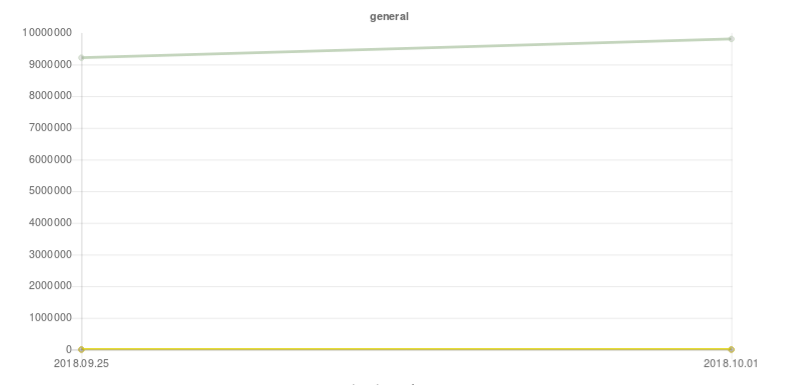
\includegraphics[width=17cm,height=8.274cm]{bilder/BilderAnalyse-img1.png}
\end{figure}
\begin{figure}
\centering
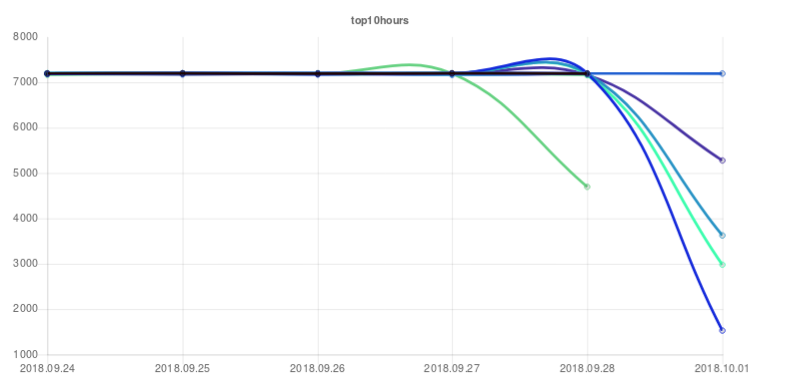
\includegraphics[width=17cm,height=8.056cm]{bilder/BilderAnalyse-img2.png}
\end{figure}
\begin{figure}
\centering
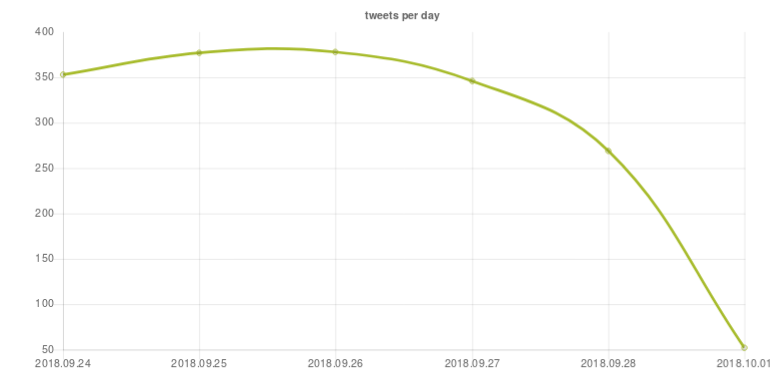
\includegraphics[width=17cm,height=8.322cm]{bilder/BilderAnalyse-img3.png}
\end{figure}

\begin{figure}
\centering
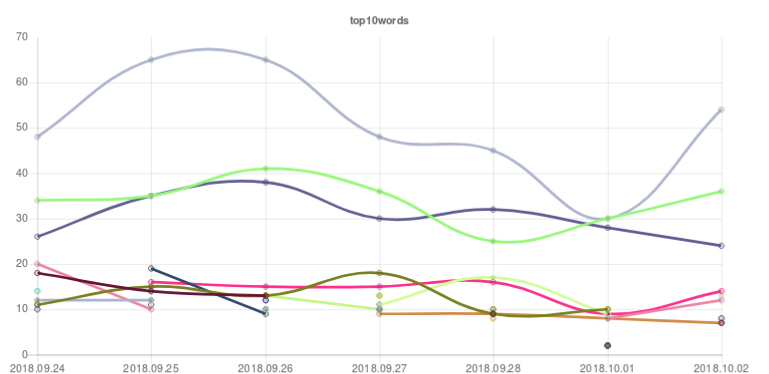
\includegraphics[width=17cm,height=8.267cm]{bilder/BilderAnalyse-img4.png}
\end{figure}
\begin{figure}
\centering
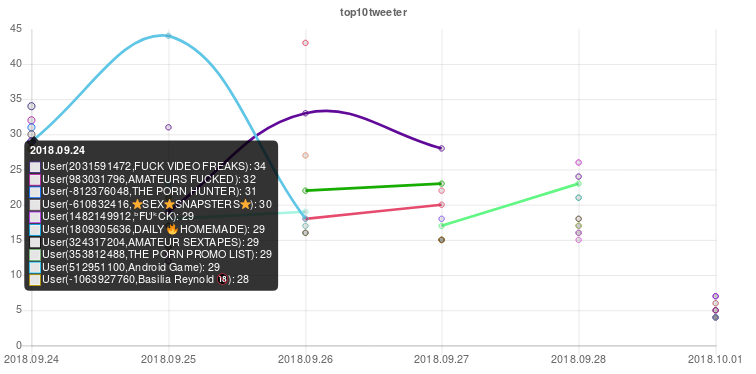
\includegraphics[width=17cm,height=8.408cm]{bilder/BilderAnalyse-img5.png}
\end{figure}
\begin{figure}
\centering
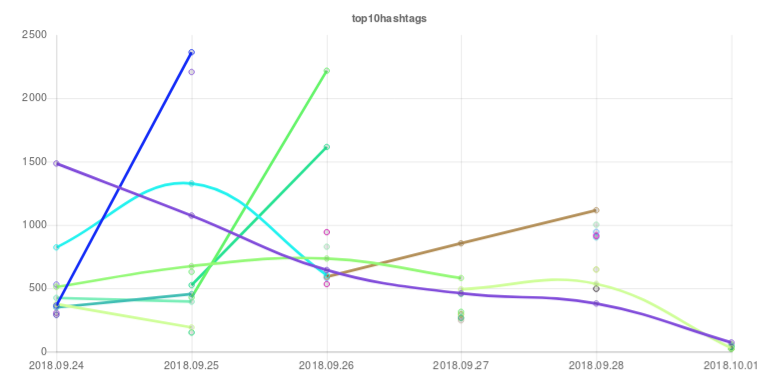
\includegraphics[width=17cm,height=8.645cm]{bilder/BilderAnalyse-img6.png}
\end{figure}


\end{document}



\section{Analytics Provisioning Service}

Für die Bereitstellung der Analysedaten ist der Micro Service \textit{Analytics Provisioning Service} zuständig. 
Dieser liest auf Anfrage Analysedaten aus Cassandra und bereitet diese für die Darstellung im Frontend auf.
In Batchanalyse werden die Ergebnisse geordnet in einer Tabelle pro Analyse gelegt, diese werden einfach nur für die letzten 14 Tage gelesen. Ergebnisse, die weiter in der Vergangenheit liegen, werden zur Zeit nicht bereit gestellt, dies ist theoretisch aber möglich.
Da Cassandra keine Counter als sekundäre Keys unterstützt und nicht für Sortierungen von großen Datenmengen ausgelegt ist,
die Analysedaten aus dem Stream jedoch unsortiert und nicht gefiltert vorliegen, war der naive Ansatz diese mittels einer  user-defined function in Cassandra pro Anfrage zu sortieren. Dies ist aber mit steigenden Tweetzahlen sehr aufwändig und könnte z.B. durch weitere Umsetzungen mit Spark ersetzt werden.

Die Kommunikation passiert auch hier über Kafka und festgelegte Topics.
Es lassen sich beliebig viele Instanzen des Services starten, die Kommunikation skaliert automatisch über die gewählte Kommunikationsarchitektur.

Für die Umsetzung wurde die Platform Node.js mit TypeScrict verwendet. 
\chapter{Conclusion}
Write here you conclusions






\blankpage

% usare questo invece di usare \appendix perchè l'altro dà un ref sbagliato sul primo link dell'indice
\changelocaltocdepth{0}
\begin{appendices}
	%\chapter{Glossary}
\label{appendixA}
Just comment \verb|\chapter{Glossary}
\label{appendixA}
Just comment \verb|\chapter{Glossary}
\label{appendixA}
Just comment \verb|\input{AppendixA-Glossary.tex}| in Masterthesis.tex if you don't need it!

\begin{longtable}{p{2.5cm}p{9.5cm}}

\huge{\textbf{Symbols}}& \\
\hline
\\
\$ & US. dollars. \\
\\
\\
\huge{\textbf{A}}& \\
\hline
\\
A& Meaning of A.\\
\\
\\
\huge{\textbf{B}}& \\
\hline
\\

\\
\\
\huge{\textbf{C}}& \\
\hline
\\

\\
\\
\huge{\textbf{D}}& \\
\hline
\\

\\
\\
\huge{\textbf{E}}& \\
\hline
\\

\\
\\
\huge{\textbf{F}}& \\
\hline
\\

\\
\\
\huge{\textbf{G}}& \\
\hline
\\
\\
\\
\huge{\textbf{H}}& \\
\hline
\\

\\
\\
\huge{\textbf{I}}& \\
\hline
\\

\\
\\
\huge{\textbf{J}}& \\
\hline
\\

\\
\\
%\huge{\textbf{K}}& \\
%\hline
%\\
%\\
%\\
%\huge{\textbf{L}}& \\
%\hline
%\\
%\\
%\\
\huge{\textbf{M}}& \\
\hline
\\

\\
\\
\huge{\textbf{N}}& \\
\hline
\\

\\
\\
%\huge{\textbf{O}}& \\
%\hline
%\\
%\\
%\\
\huge{\textbf{P}}& \\
\hline
\\

\\
\\
\huge{\textbf{Q}}& \\
\hline
\\

\\
\\
\huge{\textbf{R}}& \\
\hline
\\

\\
\\
\huge{\textbf{S}}& \\
\hline
\\

\\
\\
\huge{\textbf{T}}& \\
\hline
\\

\\
\\
\huge{\textbf{U}}& \\
\hline
\\

\\
\\
\huge{\textbf{V}}& \\
\hline
\\

\\
\\
\huge{\textbf{W}}& \\
\hline
\\

\\
\\
\huge{\textbf{X}}& \\
\hline
\\

\\
\\
%\huge{\textbf{Y}}& \\
%\hline
%\\
%\\
%\\
%\huge{\textbf{Z}}& \\
%\hline
%\\
%\\
%\\
\end{longtable}



| in Masterthesis.tex if you don't need it!

\begin{longtable}{p{2.5cm}p{9.5cm}}

\huge{\textbf{Symbols}}& \\
\hline
\\
\$ & US. dollars. \\
\\
\\
\huge{\textbf{A}}& \\
\hline
\\
A& Meaning of A.\\
\\
\\
\huge{\textbf{B}}& \\
\hline
\\

\\
\\
\huge{\textbf{C}}& \\
\hline
\\

\\
\\
\huge{\textbf{D}}& \\
\hline
\\

\\
\\
\huge{\textbf{E}}& \\
\hline
\\

\\
\\
\huge{\textbf{F}}& \\
\hline
\\

\\
\\
\huge{\textbf{G}}& \\
\hline
\\
\\
\\
\huge{\textbf{H}}& \\
\hline
\\

\\
\\
\huge{\textbf{I}}& \\
\hline
\\

\\
\\
\huge{\textbf{J}}& \\
\hline
\\

\\
\\
%\huge{\textbf{K}}& \\
%\hline
%\\
%\\
%\\
%\huge{\textbf{L}}& \\
%\hline
%\\
%\\
%\\
\huge{\textbf{M}}& \\
\hline
\\

\\
\\
\huge{\textbf{N}}& \\
\hline
\\

\\
\\
%\huge{\textbf{O}}& \\
%\hline
%\\
%\\
%\\
\huge{\textbf{P}}& \\
\hline
\\

\\
\\
\huge{\textbf{Q}}& \\
\hline
\\

\\
\\
\huge{\textbf{R}}& \\
\hline
\\

\\
\\
\huge{\textbf{S}}& \\
\hline
\\

\\
\\
\huge{\textbf{T}}& \\
\hline
\\

\\
\\
\huge{\textbf{U}}& \\
\hline
\\

\\
\\
\huge{\textbf{V}}& \\
\hline
\\

\\
\\
\huge{\textbf{W}}& \\
\hline
\\

\\
\\
\huge{\textbf{X}}& \\
\hline
\\

\\
\\
%\huge{\textbf{Y}}& \\
%\hline
%\\
%\\
%\\
%\huge{\textbf{Z}}& \\
%\hline
%\\
%\\
%\\
\end{longtable}



| in Masterthesis.tex if you don't need it!

\begin{longtable}{p{2.5cm}p{9.5cm}}

\huge{\textbf{Symbols}}& \\
\hline
\\
\$ & US. dollars. \\
\\
\\
\huge{\textbf{A}}& \\
\hline
\\
A& Meaning of A.\\
\\
\\
\huge{\textbf{B}}& \\
\hline
\\

\\
\\
\huge{\textbf{C}}& \\
\hline
\\

\\
\\
\huge{\textbf{D}}& \\
\hline
\\

\\
\\
\huge{\textbf{E}}& \\
\hline
\\

\\
\\
\huge{\textbf{F}}& \\
\hline
\\

\\
\\
\huge{\textbf{G}}& \\
\hline
\\
\\
\\
\huge{\textbf{H}}& \\
\hline
\\

\\
\\
\huge{\textbf{I}}& \\
\hline
\\

\\
\\
\huge{\textbf{J}}& \\
\hline
\\

\\
\\
%\huge{\textbf{K}}& \\
%\hline
%\\
%\\
%\\
%\huge{\textbf{L}}& \\
%\hline
%\\
%\\
%\\
\huge{\textbf{M}}& \\
\hline
\\

\\
\\
\huge{\textbf{N}}& \\
\hline
\\

\\
\\
%\huge{\textbf{O}}& \\
%\hline
%\\
%\\
%\\
\huge{\textbf{P}}& \\
\hline
\\

\\
\\
\huge{\textbf{Q}}& \\
\hline
\\

\\
\\
\huge{\textbf{R}}& \\
\hline
\\

\\
\\
\huge{\textbf{S}}& \\
\hline
\\

\\
\\
\huge{\textbf{T}}& \\
\hline
\\

\\
\\
\huge{\textbf{U}}& \\
\hline
\\

\\
\\
\huge{\textbf{V}}& \\
\hline
\\

\\
\\
\huge{\textbf{W}}& \\
\hline
\\

\\
\\
\huge{\textbf{X}}& \\
\hline
\\

\\
\\
%\huge{\textbf{Y}}& \\
%\hline
%\\
%\\
%\\
%\huge{\textbf{Z}}& \\
%\hline
%\\
%\\
%\\
\end{longtable}



\blankpage
	\chapter{Cassandra}
\label{appendix:Cassandra}
Cassandra ist eine NoSql Datenbank, die nach dem Wide-Column Model konzipiert ist. Cassandra vereint verschieden Eigenschaften von Googles BigTable \cite{bigtable} und Amazons Dynamo \cite{dynamo}. Sie wurde 2010 von Facebook entwickelt, um das Inbox Search Problem zu lösen \cite{cassandra}. Es ist eine verteilte Datenbank, die sich unter dem CAP-Theorem als AP charakterisieren lässt, wobei man das Level an Konsistenz manuell einstellen kann.

\section{Daten Model}
\label{sec:DM}
Das Daten Modell von Cassandra entspricht dem von BigTable, also dem Wide-Column Modell. Dies beruht im Wesentlichen, wie alle Arten an NoSql Datenbank Modellen auf Key-Value-Stores. Dabei wird für einen Primary Key jeweils eine Reihe mit Column-Families definiert. Die Column-Families bestehen wiederum aus einem Key, der sie beschreibt, und einem Value der dann den Wert angibt. Der Wert kann allerdings wieder eine Menge an Column-Families sein, wodurch es möglich ist Column-Families beliebig zu verschachteln. Es wird bei der Initialisierung angegeben welchen Typ der Wert hat, Verschachtlung wird über benutzerdefinierte Typen erzeugt.
\begin{figure}[htbp!]
	\centering
	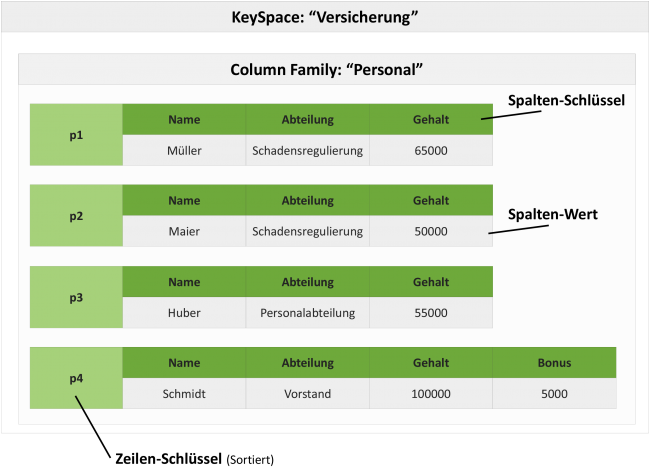
\includegraphics[scale=0.45]{pics/colfam.png}
	\figuresource{\url{http://wi-wiki.de/doku.php?id=bigdata:spaltendb}}
	\caption{Beispiel Daten Modell}
	\label{fig:bspDM}

\end{figure} Column-Families, die wiederum Column-Families beinhalten, bezeichnet man als Super-Column-Families. Bei Cassandra werden bei der Initialisierung einer Tabelle, die auch nichts anderes ist als eine Super-Column-Family, alle möglichen Column-Families angegeben. Sie definiert darüber hinaus den Primary Key über den auf die Werte der Column-Families zugegriffen werden können. Im Unterschied zu herkömmlichen SQL Tabellen ist es aber möglich Werte für diese zu unterschlagen, wie in Abbildung \ref{fig:bspDM} für p1 - p3 dargestellt.\\ 
Ein KeySpace stellt die oberste Schicht des Datenmodells dar. Für den KeySpace werden bei der Initialisierung eine Replikationsstrategie und eine Anzahl Replikas angegeben, die zu erstellen sind. Diese gelten dann für alle Tabellen, die unter dem KeySpace erstellt werden.

\section{System}
Implementiert ist Cassandra in Java. Darauf aufbauend sind auch die Basis Java Typen verfügbar. Die Daten werden von Cassandra redundant auf verschiedene Instanzen verteilt. Systemnachrichten werden dabei über UDP verschickt, Anwendungsnachrichten, also Nachrichten, die mit den Daten zu tun haben, per TCP um den Verlust von Nachrichten zu vermeiden. Bei den Systemnachrichten ist dies zu verkraften.

\subsection{Partitionierung}
Die Partitionierung orientiert sich an der von Dynamo \cite{dynamo}. Cassandra benutzt genauso wie Dynamo Consistent-Hashing, um Daten auf die verschiedenen Instanzen zu verteilen. Dabei erhalten die verschiedenen Instanzen einen Wert, der sie uniform über einen vordefinierten Wertebereich verteilt, wie in Abbildung \ref{fig:uniformHashing} abgebildet. Consistent-Hashing macht aus dem Wertebereich einen Ring, über den dann die Daten auf die Instanzen wie folgt verteilt werden. Aus einem Datum wird über die Hashfunktion ein Hash-wert berechnet. Das Datum wird dann auf der Instanz abgespeichert, deren Wert auf dem Ring aufsteigend als nächstes kommt. Dieses Verfahren kann zu einer ungleichen Verteilung der Daten auf die Instanzen führen, sodass dadurch die Performance des Systems ineffizient wird. Cassandra löst diese Problem anders als Dynamo dadurch, dass die Werte der Instanzen an die Verteilung der Daten angepasst werden, wie in Abbildung \ref{fig:adaptedHashing} dargestellt. So sind zwar einige Instanzen für einen größeren Wertebereich zuständig, andererseits kommen in diesem größeren Wertebereich weniger Daten vor, sodass die Daten uniform auf die Instanzen verteilt werden. Wird der Datensatz zu groß, skaliert Cassandra, indem eine Instanz im Consistent-Hashing Ring zwischen den Knoten mit den meisten Daten eingefügt wird. Danach werden die Bereiche wieder so angepasst, dass alle Instanzen ungefähr gleich belastet sind.
\begin{figure}[htbp!]
	\centering
	\begin{subfigure}[c]{0.49\textwidth}
		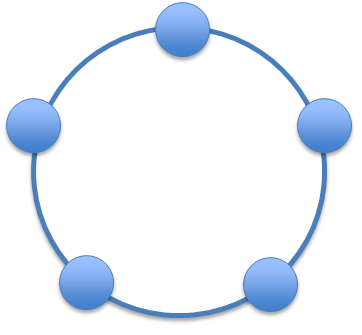
\includegraphics[scale=0.5]{pics/uniformHashing.png}
		\subcaption{Consistent-Hashing uniform distributed instances}
		\label{fig:uniformHashing}
	\end{subfigure}
	\begin{subfigure}[c]{0.49\textwidth}
		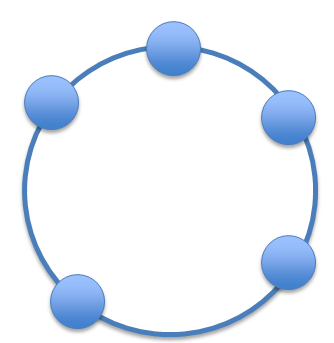
\includegraphics[scale=0.5]{pics/adaptedHashing.png}
		\subcaption{Consistent-Hashing adapted distribution of instances}
		\label{fig:adaptedHashing}
	\end{subfigure}
	\caption{Consistent-Hashing Ring}
\end{figure}

\subsection{Replikation}
Die Art der Replikation in Cassandra ist vom Benutzer konfigurierbar. Die Anzahl der Replikas und die Replikationsstrategie wird durch den KeySpace festgelegt. Dabei kann man zwischen SimpleStrategy und NetworkTopologyStrategy auswählen. Die SimpleStrategy repliziert ohne auf die Netzwerkstruktur einzugehen. Somit beugt sie weniger stark potentiellem Datenverlust vor und sollte daher nur für Test-Zwecke benutzt werden. Sei N die Anzahl Replikas, werden die Daten immer auf die N-1 Nachfolgeknoten repliziert. Bei der NetworkTopologyStrategy wird die Hierarchie von Datacentern und drin enthalten Racks bei der Verteilung betrachtet wird. Somit wird diese Strategie auch für das Deployment empfohlen. Innerhalb dieser Strategie kann man sich wiederum zwischen Rack Aware und Datacenter Aware entscheiden. Dabei werden die Replikas entweder auf verschiedene Racks oder Datacenter verteilt, um die höchst mögliche Datensicherheit zu gewährleisten. Diese Strategien beziehen sich auf den Koordinator, also die Hauptinstanz einer Partition von Daten, da dieser für die Replikation zuständig ist.
Bei der Bestimmung eines Koordinators wird Zookeeper verwendet. Dadurch sind alle Netzwerkänderungen und -konfigurationen persistent gespeichert, da Zookeeper die Konfigurationen jedes Knotens automatisch persistent speichert. Zur Kommunikation werden bei Zookeeper Gossip Algorithmen verwendet.

\subsection{Persistenz}
Persistenz erreicht Cassandra über ein ähnliches System wie BigTable \cite{bigtable}. Zunächst gibt es die MemTable, die im Hauptspeicher gehalten wird und als Cache fungiert. Sie besitzt eine Konfiguration einer Schranke, ab der die MemTable auf die Platte persistiert wird. Auf der Platte gibt es die SSTable, Bloom Filter, index file, compression file und statistics file. Die Daten werden in eine SSTable geschrieben, also eine eigene Datei geschrieben, wenn sie noch nicht vorhanden sind. Wenn dies nicht der Fall ist, wird der betreffende Teil einer SSTable in die MemTable geladen, alle Operationen ausgeführt und die Daten wieder zurück auf die Platte geschrieben. Der Bloom Filter verhindert unnötige Lookups in nicht relevante SSTables. Der Index beschleunigt den Lookup innerhalb einer SSTable. Damit man nicht viele kleine SSTable-Dateien hat werden zwei SSTable, durch einen merge-Prozess immer dann zusammengefasst, wenn eine mindestens halb so groß ist wie die andere. Vorhandene SSTable Files können zusätzlich noch komprimiert werden.

\section{CQL}
Mit CQL (Cassandra Query Language) gibt es eine auf Cassandra zugeschnittene SQL-ähnliche Abfragesprache, die es den Anwendern konventioneller Datenbanken deutlich leichter macht mit Cassandra zu arbeiten. Dabei ist es wichtig zu wissen, dass CQL bei weitem nicht so ausdrucksstark ist wie SQL. Das liegt daran, dass CQL im wesentlich eine abstrakte API für das Cassandra Datenmodell darstellt. In CQL sind normale Datenbank Typen wie int, text, etc. möglich, allerdings kann man auch von Collections wie List, Set und Map Gebrauch machen, da es dafür direkte Java Typen gibt. Des Weiteren ist es möglich eigene Typen zu definieren, wie schon in Abschnitt \ref{sec:DM} beschrieben.\\
\begin{figure}[htbp!]
	\centering
	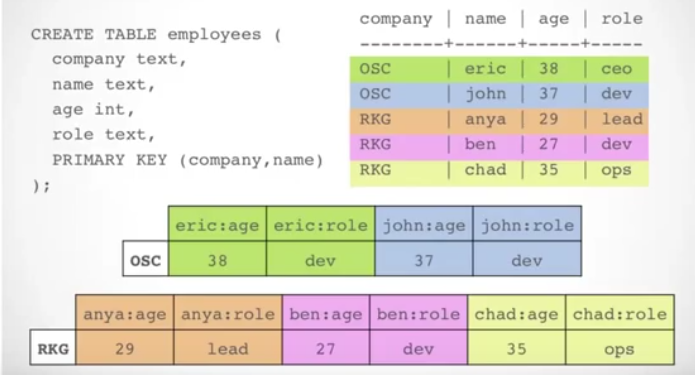
\includegraphics[scale=0.7]{pics/cql_mapping.png}
	\figuresource{\url{https://www.youtube.com/watch?v=UP74jC1kM3w}}
	\caption{CQL Mapping}
	\label{fig:mapping}
\end{figure}
Tabellen und Spalten werden wie ebenso in Abschnitt \ref{sec:DM} beschrieben durch Column-Families dargestellt. und wie in SQL erzeugt. Dabei wird ein Primary Key benötigt, der dann als Row Key fungiert. Es kann nur über diesen Row Key auf die Zeilen zugegriffen werden. Deshalb kann man in der WHERE-Klausel in CQL auch nur Elemente des Primary Key angeben. Auf diesen Elementen wird durch die Indizierung schon beim Speichern in Cassandra eine Sortierung berechnet was die Anfragen deutlich perfomanter macht. Für alle anderen Spalten der Zeile wäre dies also nicht performant und wird von CQL nicht gestattet. Die Spalten und Zeilen werden wie folgt auf das Cassandra Datenmodell abgebildet.\\
Der erste Teil des Primary Keys bildet, wie man sehen kann, den Row Key, die restlichen Teile werden mit ihren Werten in die Beschreibung der Column-Families integriert, so wie im unteren Teil in Abbildung \ref{fig:mapping} beschrieben. Somit werden alle Zeilen mit dem gleichen ersten Teil des Primary Keys in der gleichen Zeile abgespeichert. Über dieses Mapping ist es möglich eine tabellenartige Abstraktion zu erzeugen, die sich durch CQL ausdrückt und Anwendern ein aus SQL bekanntes Interface bietet.

	\chapter{Big Table}
\label{bigTable}
Some text.

\section{Einführung}
Täglich kommen mehrere Petabytes an Daten von über 60 Google Anwendungen zusammen. Dafür verantwortlich sind mehr als 1000 Computer die untereinander vernetzt sind. Um diese Daten verwalten zu können wurde Bigtable ins Leben gerufen. Das Ziel der Datenbank war es in vielen Bereichen anwenden zu können. Dazu sollte es Skalierbar sein sowie eine hohe Performance und Verfügbarkeit besitzen.


\section{Datenmodell}
Bigtable ist eine verteiltes, persistentes multidimensionale sortierte Map. Diese Map ist indexiert über eine row key, columen key und einem timestamp. Jeder Wert in dieser Map ist ein Array mit Bytes. Das folgende Datenmodell soll eine Speicherung von Webseiten veranschaulichen.

\begin{figure}[!htpb]
	\centering
	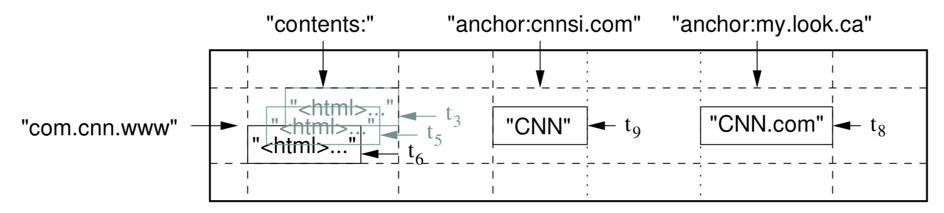
\includegraphics[]{pics/bigtable_schema.png}
	\caption {Tabellen Beispiel}	
\end{figure}

Das Datenmodell besteht aus zwei Familien dem Inhalt und den Ankerpunkten. Die erste Familie beinhaltet den Inhalt der Webseite, mit drei unterschiedlichen Zeitstempeln (t3,t5,t6). Drei unterschiedliche Zeitstempeln bedeutet, dass die Website www.cnn.com in drei unterschiedlichen Versionen abgespeichert wurde. Die Anker Familie beinhaltet jeweils nur eine Version. Den Anker mit „CNN.com“ mit dem Zeitstempel t8 und dem Anker „CNN“ mit dem Zeitstempel t9. 
 
\paragraph{Rows}
Bigtable speichert Daten in lexikopgrahischer reihenfolge und sortiert diese nach Zeilen. Eine row range beinhaltet alle gleichnamigen URL’s, so dass alle mit der gleichen Domain zusammen abgespeichert werden. Das vereinfacht die Analyse und das Hosting der gleichnamigen Domains und macht dies zudem effizienter.

\paragraph{Column families}
Verschieden column keys werden in eine gemeinsame Gruppe gespeichert. Das nennt man column families. Alle Daten, welche in der gleichen Gruppe gespeichert werden sind vom gleichen typ. Bevor Daten in einer Gruppe gespeichert werden können, muss diese column family als erstes erstellt werden.

\paragraph{Timestamp}
Jede Zelle in Bigtable kann mehrere Versionen der gleichen Daten beinhalten. Dieser Versionen werden indexiert durch den Zeitstempel (timestamp). Der Zeitstempel ist bis auf die Micro Sekunde genau. Durch die „two per-column-family“ kann der Benutzer festlegen, wie viele Versionen der gleichen Daten gespeichert werden sollen. Alle weiteren Versionen werden automatisch gelöscht.

\paragraph{API}
Die API von Bigtable ermöglicht das erstellen und löschen von Tabellen und Spaltennamen, sowie das ändern von Tabellen, Cluster und Metadaten einer Spaltenfamilien. Das folgende Codebeispiel wurde in C++ geschrieben und Verändert den Inhalt der Tabelle Webtable. 

\begin{figure}[!htpb]
	\centering
	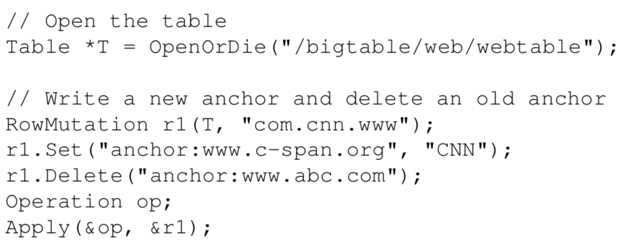
\includegraphics[]{pics/bigtable_api.png}
	\caption {Zugriffs Beispiel mit der BigTable API}	
\end{figure}

Der Code verändert die Spalte „com.cnn.www“ und fügt einen neuen Anker hinzu. Im nächsten Schritt wird ein vorhandener Anker „anchor:www.abc.com“ gelöscht und festgeschrieben.


\paragraph{Building Blocks}
Bigtable ist auf mehreren anderen Teilen der Google-Infrastruktur aufgebaut. Zum Beispiel benutzt Bigtable das verteilte Google File System (GFS). Welches für die Speicherung von Logs und Daten verantwortlich ist. Ein Bigtable Cluster operiert typischerweise auf einem verteilten Pool von Computern. Auf diesem Pool laufen eine breite sparte von verschiedenen Anwendungen. Bigtable basiert auf einem Cluster Management System für Zeit-Planung-Jobs, Ressourcenmanagements auf geteilten Computer, agieren mit Computerfehlern und dem Anzeigen des Computer Status. Das SSTable Format stellt eine persistente, geordnete unveränderliche Abbildung von Schlüsseln zu Werten zur Verfügung, wobei sowohl Schlüssel als auch Werte willkürliche Bytefolgen sind. Operationen werden bereitgestellt, um den Wert zu suchen, der einem bestimmten Schlüssel zugeordnet ist.

\paragraph{Implementation}
Bigtable besteht aus drei Haupt Komponenten, einer Bibliothek, einem Master Server und vielen weiteren tablet servern. Die Bibliothek ist in jeden Client verlinkt, somit kann der Client auf alle Funktionen zugreifen. Der Master Server wird zufällig ausgewählt. Dieser teilt den tablet servern die tablets zu. Außerdem ist für die Verteilung der Lasten zuständig und ist für die garbage collection. Sobald eine Tabelle zu groß wird, wird diese von einem tablet server gesplittet. So wird sichergestellt, dass eine Tabelle nie größer als 100-200 MB ist.

\paragraph{Tablet location}
Um Daten zu speichern, verwendet Google bei Bigtable eine „three-level hirarchy“. Das erste Level ist eine Datei, welches auch das Chubby file genannt wird, dort wird der Speicherort des root tablets hinterlegt. Das root tablet beinhaltet alle Speicherorte aller tablets in einer METADATA Tabelle. Das spezielle an dieser Tabelle ist, dass egal wie groß sie wird, diese niemals geteilt wird. Somit wird sichergestellt, dass die „three-level hirarchy“ eingehalten wird. Die METADATA Tabellen speichern die Orte aller anderen tablets in einer Tabelle ab.

\paragraph{Tablet Zuweisung}
Jedes tablet ist zu einem Zeitpunkt immer nur einem tablet server zugeordnet. Der Master server verfolgt die lebenden tablet servern und die aktuell zugeordneten tablets zu den tablet servern inklusive aller unzugeordneten tablet servern.
Beim Start einer Bigtable führt der Master Server folgende Schritte aus:

\begin{enumerate}
	\item Wählt einen einzigartigen Master Lock in Chubby
	\item Scannt die Server Verzeichnisse um die lebenden tablet server zu finden
	\item Kommuniziert mit den vorhandenen tablet server um bereits zugeordnete tablets zu identifizieren
	\item Master scannt METADATA Tabelle um die vorhandene Zugehörigkeiten zu lernen
\end{enumerate}

\paragraph{Tablet serving}
Ein persistenter Zustand eines tablets wird in GFS gespeichert. Alle Updates werden auf „well-formed“ geprüft und anschließend in einem commit-log gespeichert. Die neusten Updates werden in eine memtable gespeichert, ältere updates werden in die SSTable geschrieben. Wenn Daten aus dem tablet server abgefragt werden muss ein merge zwischen den neuen Daten in der memtable sowie den älteren Daten in der SSTable erstellt werden.

\paragraph{Compaction}
Je mehr Daten gespeichert werden, umso größer wird die memtable. Damit diese tabelle nicht zu groß wird, gibt es ein „minor compaction“. Diese Funktion friert eine memtable ein sobald diese eine bestimmte Größe erreicht hat und erstellt eine neue memtable. Die gefrorene memtable wird zu einer SSTable konvertiert. Je mehr Daten gespeichert werden, desto unordentlicher wird die Ansammlung von SSTable. Um die SSTable zu sortieren wird periodisch ein „merging compaction“ ausgeführt. Dies strukturiert die SSTable neu und es werden Ressourcen, durch die Löschung von Daten, freigegeben. Außerdem werden gelöschte Daten endgültig gelöscht, das ist wichtig für Services, welche sensible Daten beinhalten.

\section{Refinments}
Um die hohe Performance, Verfügbarkeit und Zuverlässigkeit beizubehalten, werden einige Verbesserungen (refinments) benötigt.

\paragraph{Lokale Gruppen}
Gruppierung erspart Zugriffszeit. Zum Beispiel bei dem Datenmodell Webseite. Die „page metadate“ und „content“ der Webseite werden in einer anderen gruppe gespeichert. So muss eine Anwendung, welche nur die Metadaten möchte, nicht durch den kompletten Inhalte einer Seite iterieren.
Zudem gibt es Tuningparameter, welche bestimmten ob Daten in den Arbeitsspeicher geladen werden um die Zugriffszeit zu minimieren.

\paragraph{Kompression}
Ein Benutzer kann selbst bestimmen ob SSTable komprimiert wird und falls ja, in welchem Ausmaß. Jeder SSTable Block kann einzeln ausgewählt werden. Für die Komprimierung kommen die  verfahren Bentley und McLlroy’s zum Einsatz. Diese können mit 100-200Mb/s Kodiert und mit 400-1000 MB/s Enkodiert werden.

\paragraph{Caching für Lesezugriffe}
Für das Caching von Lesezugriffe gibt es zwei verfahren. Der Scan Cache (high-level), speichert key-value Paare und liefert eine SSTable zurück. Das Block Cache (lover-level) verfahren speichert SSTable Blocks, die von der GFS gelesen werden.

\paragraph{Bloom Filter}
Benutzer legt selbst fest ob ein Filter zum Einsatz kommt. Der Vorteil eines Filters liegt darin, dass wenn Daten gesucht werden, nicht jede SSTable nach den bestimmten Daten durchsucht werden muss. Ein Bloom Filter erlaubt es, nach einer bestimmten Art von row/column paaren zu fragen, ob diese in einer SSTable gespeichert sind.

\paragraph{Beschleunigte tablet Wiederherstellung}
Wenn der Master ein tablet von einem Server zu einem anderen Server verschiebt, führt der Ursprungs Server erst ein „minor compaction“ aus um die Ladezeit für den neuen tablet server zu verkürzen.

\paragraph{Unveränderlichkeit ausnutzen}
Es können nur Daten verändert, welche in der memtable stehen. Daten in der SSTable können nicht verändert werden. Das macht man sich zu nutzen indem man keine Synchronisation braucht, wenn auf die Daten zugegriffen wird. Memtable sind die einzigen Daten auf die man schreiben kann und gleichzeitig lesen. Damit es zu keinen komflikten kommt, setzt Bigtable hier auf „Copy-on-write“. 

\section{Performance Auswertung}
\begin{figure}[!htpb]
	\centering
	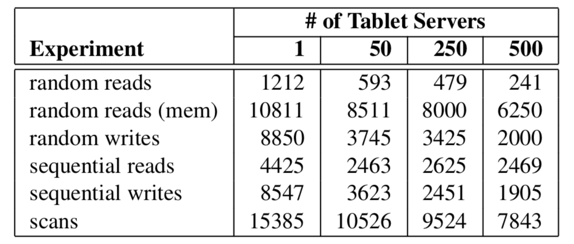
\includegraphics[]{pics/bigtable_performance.png}
	\caption {Percormance Übersicht}	
\end{figure}
Die Performance wird hauptsächlich durch die verwendete CPU (2ghz) begrenzt. Zudem kann man erkennen, dass bei einem tablet server der Durchsatz bei ca. 75MB/s liegt (1000 bytes * 64 KB Block size = 75 MB/s). Damit der Durchsatz bei einem Single tablet server erhöht wird, wird die die SSTable größe in der regel von 64KB auf 8kb gesenkt. 
Zudem wird erkannt, dass der Durchsatz nicht Linear ansteigt. Bei einer Erhöhung der tablet server von eins auf 500 liegt die Erhöhung des Durchsatzes bei gerade mal dem 300 fachen (10811 / (500 * 6250) = 350). Diese Begrenzung liegt wie bei einem tablet server an der CPU der tablet servern.

	\chapter{Dynamo}
\label{appendiceC}


\section{Problemstellung und Einordnung}
Amazon wickelt Bestellungen von Kunden rund um die Welt ab. Hierfür benötigt Amazon ein hochverfügbares System, das sicherstellt, dass jederzeit Bestellungen entgegen genommen werden können. Es werden also viele Rechenzentren benötigt, um diese Last zu tragen. Bei der Auswahl von Rechnern für diese Rechenzentren setzt Amazon allerdings nicht auf hochverfügbare Spezialhardware, sondern setzt handelsübliche Rechner ein. Um dennoch eine möglichst hohe Verfügbarkeit garantieren zu können, hat Amazon die verteilte Datenbank Dynamo entwickelt, die in \cite{dynamo} beschrieben wurde und in diesem Kapitel vorgestellt werden soll. \\ 
\\
Dynamo ist dafür konzipiert, bei Verfügbarkeit einer minimalen Anzahl an Knoten, Schreibvorgänge annehmen zu können. Dynamo ist also partitionierungstolerant und hoch verfügbar, kann Datenkonsistenz aber nur unter bestimmten Bedingungen garantieren. 
\section{Datenmodell}
Dynamo ist ein Key-Value-Store. Werte werden also unter einem Schlüssel abgelegt und können nur über diesen Schlüssel wieder abgefragt werden. Komplexere Anfragen sind daher nicht möglich. Der Wert, der hinterlegt wird, muss keinem festen Datenschema entsprechen - es können beliebige Binärdaten gespeichert werden.

\section{Architektur}

\subsection{Konsistentes Hashing}
Um die Daten den Knoten zuzuordnen, verwendet Dynamo konsistentes Hashing. Hierbei wird für jeden Schlüssel ein MD5 128 Bit Hash-Wert gebildet. Den Knoten wird ebenfalls ein Wert zwischen $0$ und $2^{128}$ zugeordnet. Ein Schlüssel-Wert-Paar wird auf dem Knoten gespeichert, dem der nächst höhere Wert ausgehend vom Hash-Wert des Schlüssels zugeordnet wurde. Gibt es keinen Knoten, der einen höheren Wert hat, wird das Schlüssel-Wert-Paar auf dem Knoten mit dem kleinsten Wert gespeichert.\\
Visuell lässt sich dieses Verfahren wie in Abbildung \ref{fig:bspKonHash} mithilfe eines Kreises darstellen. Jeder Position auf dem Kreis wird im Uhrzeigersinn beginnend am obersten Punkt des Kreises ein Wert von $0$ bis $2^{128}$ zugeordnet. Knoten wie Schlüssel können dann anhand ihres Hash-Wertes auf dem Kreis platziert werden. Ein Schlüssel-Wert-Paar wird auf dem Knoten gespeichert, der auf dem Kreis an der nächsten Stelle im Uhrzeigersinn liegt.
\begin{figure}
	\caption{Beispiel für konsistentes Hashing. Die Daten sollen auf vier Knoten verteilt werden, wobei die Knoten gleichmäßig auf dem Kreis platziert sind.}
	\label{fig:bspKonHash}
	\centering
	\begin{tikzpicture}
		\draw (0,0) circle (2cm);
		\node[fill=black,circle,scale=0.5] (zero) at (0,2) {};
		\node[above] at (zero) {$2^{128}$ $0$};
		\node[fill=black,circle,scale=0.5] (A) at (1.41,1.41) {};
		\node[below left] at (A) {hash(A)};
		\node[fill=black,circle,scale=0.5] (K2) at (2,0) {};
		\node[fill=black,circle,scale=0.5] (B) at (1.79,-0.89) {};
		\node[left] at (B) {hash(B)};
		\node[fill=black,circle,scale=0.5] (C) at (1.41,-1.41) {};
		\node[left] at (C) {hash(C)};
		\node[fill=black,circle,scale=0.5] (K3) at (0,-2) {};
		\node[fill=black,circle,scale=0.5] (D) at (-1.79,-0.89) {};
		\node[right] at (D) {hash(D)};
		\node[fill=black,circle,scale=0.5] (K4) at (-2,0) {};
		\node[fill=black,circle,scale=0.5] (E) at (-1.79,0.89) {};
		\node[right] at (E) {hash(E)};
		\draw (3,2) rectangle (6,0.5);
		\draw (3,-2) rectangle (6,-0.5);
		\draw (-3,2) rectangle (-6,0.5);
		\draw (-3,-2) rectangle (-6,-0.5);
		\draw (zero) -- (3,2);
		\draw (K2) -- (3,-0.5);
		\draw (K3) -- (-3,-2);
		\draw (K4) -- (-3,0.5);
		\node at (4.5,1.5) {Knoten 1};
		\node at (4.5,1) {\scriptsize{Eintrag E}};
		\node at (4.5,-1) {Knoten 2};
		\node at (4.5,-1.5) {\scriptsize{Eintrag A}};
		\node at (-4.5,-1) {Knoten 3};
		\node at (-4.5,-1.5) {\scriptsize{Einträge B, C}};
		\node at (-4.5,1.5) {Knoten 4};
		\node at (-4.5,1) {\scriptsize{Eintrag D}};
	\end{tikzpicture}
\end{figure}
\subsection{Replikation}
Replikation lässt sich nun leicht realisieren, indem die Einträge nicht nur auf dem nächsten, sondern bei einem Replikationsfaktor von $n$ auf den nächsten $n$ Knoten gespeichert werden. Fällt dann ein Knoten aus, lassen sich die Einträge weiterhin auf dem jeweils nächsten Knoten auf dem Kreis auffinden. Bei einem Ausfall muss dafür gesorgt werden, dass die Bedingung, dass alle Daten auf den nächsten $n$ Knoten gespeichert sind, wieder hergestellt wird.
\subsection{Partitionierung und Verteilung}
Bei der Partitionierung aus Abbildung \ref{fig:bspKonHash} ist beim Ausfall eines Knotens das Problem, dass die nächsten $n$ Knoten (bei Replikationsfaktor $n$) die volle Last das Ausfalls tragen müssen, da die Daten, die der ausgefallene Knoten gespeichert hat, auf die nächsten $n$ Knoten repliziert werden müssen. Ist $n$ im Vergleich zur Anzahl der insgesamt verfügbaren Knoten eher klein, wäre es wünschenswert eine bessere Verteilung der Last zu erzielen. Daher platziert Dynamo die Knoten nicht direkt auf dem Kreis, sondern plaziert stattdessen virtuelle Knoten. Dabei stehen mehrere virtuelle Knoten für einen realen Knoten. Nun können die virtuellen Knoten so auf dem Kreis verteilt werden, dass auf die virtuellen Knoten eines realen Knotens die virtuellen Knoten verschiedener realer Knoten folgen. Bei dem Ausfall eines realen Knotens wird die entstehende Last also auf viele oder sogar alle realen Knoten verteilt.\\
\\
In Abbildung \ref{fig:bspKonHash} wurden die Knoten gleichmäßig auf dem Kreis verteilt. Es ließe sich nun ein Schema finden, das für virtuelle Knoten eine Verteilung auf dem Kreis bestimmt, durch die die virtuellen Knoten ebenfalls gleichmäßig auf dem Kreis verteilt werden, und dafür sorgt, dass der Ausfall eines Knotens zunächst von allen anderen Knoten getragen wird. Das Problem ist jedoch, dass das Schema nach dem Ausfall erneut ausgeführt werden müsste, um eine gleichmäßige Verteilung wieder herzustellen. Hierbei würden jedoch meist alle virtuellen Knoten neu platziert werden und es müssten viele Daten verschoben werden. Ein ähnliches Szenario würde das Hinzufügen eines Knotens hervorrufen.\\
Da der Aufwand für das Verschieben der Daten zu hoch wäre, lässt sich ein solches optimales globales Schema nicht realisieren. Stattdessen wurden von Amazon drei Strategien zur Verteilung der Daten evaluiert. Diese werden im Folgenden vorgestellt:
\subsubsection*{Strategie 1}
Die erste Strategie verteilt die virtuellen Knoten zufällig auf dem Kreis. Hierdurch lässt sich eine gute Lastverteilung bewirken, da es unwahrscheinlich ist, dass ein Knoten im Vergleich zu den anderen Knoten einen sehr viel größeren Bereich des Kreises zugewiesen bekommt. Des Weiteren ist die Wahrscheinlichkeit gering, dass auf die meisten virtuellen Knoten eines realen Knotens fast ausschließlich virtuelle Knoten eines einzigen anderen realen Knotens folgen.\\
Außerdem hat diese Strategie den Vorteil, dass das Hinzufügen eines neuen Knotens eine verteilte Operation ist: Der Knoten kann die Positionen seiner virtuellen Knoten zufällig auswählen und die realen Knoten, die die Daten seines Bereichs halten, um die Übergabe der Daten bitten. Diese Knoten können dann ihren Speicher nach Einträgen durchsuchen, die übergeben werden sollen.\\
Es wurde jedoch festgestellt, dass eben dieses Durchsuchen des Speichers eines Knotens sehr aufwändig ist, da alle Einträge überprüft werden müssen. Strategie 2 vereinfacht diesen Suchvorgang. 
\subsubsection*{Strategie 2}
Strategie 2 wurde nur für kurze Zeit eingesetzt und kann als Zwischenschritt zu Strategie 3 betrachtet werden.\\
Strategie 2 unterteilt den Kreis in gleichgroße Partitionen. Dabei muss die Anzahl der Partitionen sehr viel größer sein als die Anzahl der potentiellen virtuellen Knoten. Ein Knoten speichert immer nur die Daten einer vollen Partition. Auch Strategie 2 verteilt die virtuellen Knoten zufällig auf dem Kreis. Auf die gleiche Weise, wie bei Strategie 1 die Einträge auf die Knoten zugeordnet wurden, werden bei dieser Strategie die Partitionen den Knoten zugeordnet. Ein Knoten legt einen neuen Eintrag dann im Speicherbereich der entsprechenden Partition ab. Wird er von einem neuen Knoten aufgefordert, einen Bereich des Kreises abzugeben, muss er nicht seinen kompletten Speicher nach Einträgen durchsuchen, sondern nur die zum Bereich gehörenden Partitionen bestimmen. Hierdurch wird nicht nur der Suchaufwand beim Hinzufügen eines Knotens verringert, sondern auch der benötigte Speicher, um festzuhalten, welcher Bereich des Kreises auf welchem Knoten liegt, verringert sich immens.
\subsubsection*{Strategie 3}
Strategie 3 geht wie Strategie 2 vor, bis auf dass die Knoten nicht mehr auf dem Kreis platziert werden, sondern die Partitionen den Knoten direkt zufällig zugeordnet werden. Kommt ein neuer Knoten hinzu, erhält er von jedem Knoten die gleiche Anzahl an zufällig ausgewählten Partitionen.
\subsection{Die put()- und die get()-Operation}
Mit der put()-Operation lassen sich Daten in Dynamo anlegen. Wird die put()-Operation an einem Knoten aufgerufen, informiert dieser Knoten zunächst den nächsten erreichbaren Knoten auf dem Kreis ausgehend vom Hash-Wert des Schlüssels des neuen Eintrags. Dieser Knoten ist für das weitere Verfahren verantwortlich. Hat er die Nachricht erhalten, speichert er den Eintrag und informiert die nächsten $N-1$ Knoten auf dem Kreis über den Eintrag. Hat er von $W-1$ Knoten eine Bestätigung erhalten, dass diese den Eintrag ebenfalls gespeichert haben, kann er den Nutzer informieren, dass der Eintrag gespeichert ist. Der Nutzer erhält die Bestätigung also, wenn der Eintrag auf $W$ Knoten abgelegt ist. Anschließend wartet der verantwortliche Knoten, ob er von den restlichen Knoten eine Antwort bekommt und informiert den nächsten Knoten auf dem Kreis ebenfalls über den Eintrag, falls einer der $N-1$ Knoten nicht reagiert. Das Ziel ist also, den Eintrag $N$ Mal zu speichern. \\
Bei der get()-Operation wird die Anfrage ebenfalls zunächst an den verantwortlichen Knoten übermittelt. Dieser leitet die Anfrage an $N-1$ Knoten weiter und beantwortet die Anfrage, wenn ihm die Ergebnisse von $N-1$ anderen Knoten und sein eigenes Ergebnis zur Verfügung stehen. Um Widersprüche in den Ergebnissen auflösen zu können, wird eine Versionierung der Daten benötigt.
\subsection{Versionierung}
Dynamo verändert gespeicherte Einträge nicht, sondern behandelt eine Änderung als neue Version der Daten. Dynamo verwendet Vektoruhren, um aufzulösen, welche Version eines Eintrages neuer ist. Der Zeitstempel des alten Eintrages wird bei einem Update vom Nutzer der Datenbank mitgegeben, sodass der Knoten, der für den neuen Eintrag verantwortlich ist, einen neuen Zeitstempel erstellen kann. Findet ein Knoten zwei Einträge vor, die widersprüchliche Vektoren haben, also keine Aussage getroffen werden kann, welcher Eintrag neuer ist, speichert er beide Einträge ab und bei der nächsten Anfrage werden beide Einträge dem Nutzer übergeben. Dieser muss dann den Konflikt auflösen. \\
\\
Es gibt einige Anwendungsfälle, in denen eine solche Konfliktlösung leicht ableitbar ist. So wird in \cite{dynamo} der Anwendungsfall des virtuellen Einkaufskorbs als Beispiel genannt. Hatte ein Nutzer die Version 1 seines Einkaufkorbes und hat anschließend zwei Artikel in den Einkaufskorb gelegt, wobei beim ersten Artikel basierend auf Version 1 eine Version 2 des Einkaufskorbes erstellt wurde und beim zweiten Artikel ebenfalls basierend auf Version 1 eine Version 3 erstellt wurde, so lässt sich der Konflikt zwischen Version 2 und Version 3 leicht durch das Vereinigen der beiden Einkaufskörbe lösen. Auf diese Weise kann kein hinzugefügter Artikel verloren gehen. Nur wenn ein Artikel entfernt wurde, kann es dazu kommen, dass dieser Artikel wieder im Einkaufskorb landet.
\section{Erneute Einordnung}
Mithilfe der Parameter $W$ und $R$ kann Dynamo etwas differenzierter im CAP-Theorem eingeordnet werden. Je niedriger die Parameter $W$ und $R$ sind, desto verfügbarer und partionierungstoleranter wird Dynamo. Werden beide Parameter auf $1$ gesetzt, reicht ein verfügbarer Knoten, um eine Schreiboperation durchzuführen und ein verfügbarer Knoten, der eine beliebige Version des Eintrag gespeichert hat, um eine Anfrage zu beantworten. Allerdings leidet die Konsistenz unter sehr niedrigen Werten $W$ und $R$. Werden $W$ und $R$ auf die Anzahl der Knoten gesetzt, ist Dynamo komplett konsistent, aber weder verfügbar, wenn ein Knoten ausfällt, noch partitionierungstolerant.
	

\chapter{MapReduce}
\label{MapReduce}

\section{Modell}

MapReduce ist ein generalisierter Ansatz für verteile Datenverarbeitung.
Zusätzlich wird mit MapReduce eine Laufzeitumgebung vorgeschlagen, welche für die automatische Verteilung und Parallelierung zuständig ist und außerdem Fehlerbehandlung, sowieso Kommunikation während der verteilten Berechnung abdeckt.
Folgende Übersicht basiert auf dem Paper \textit{MapReduce: Simplified Data Processing on Large Clusters} \cite{mapReduce}.


\begin{figure}[H]
	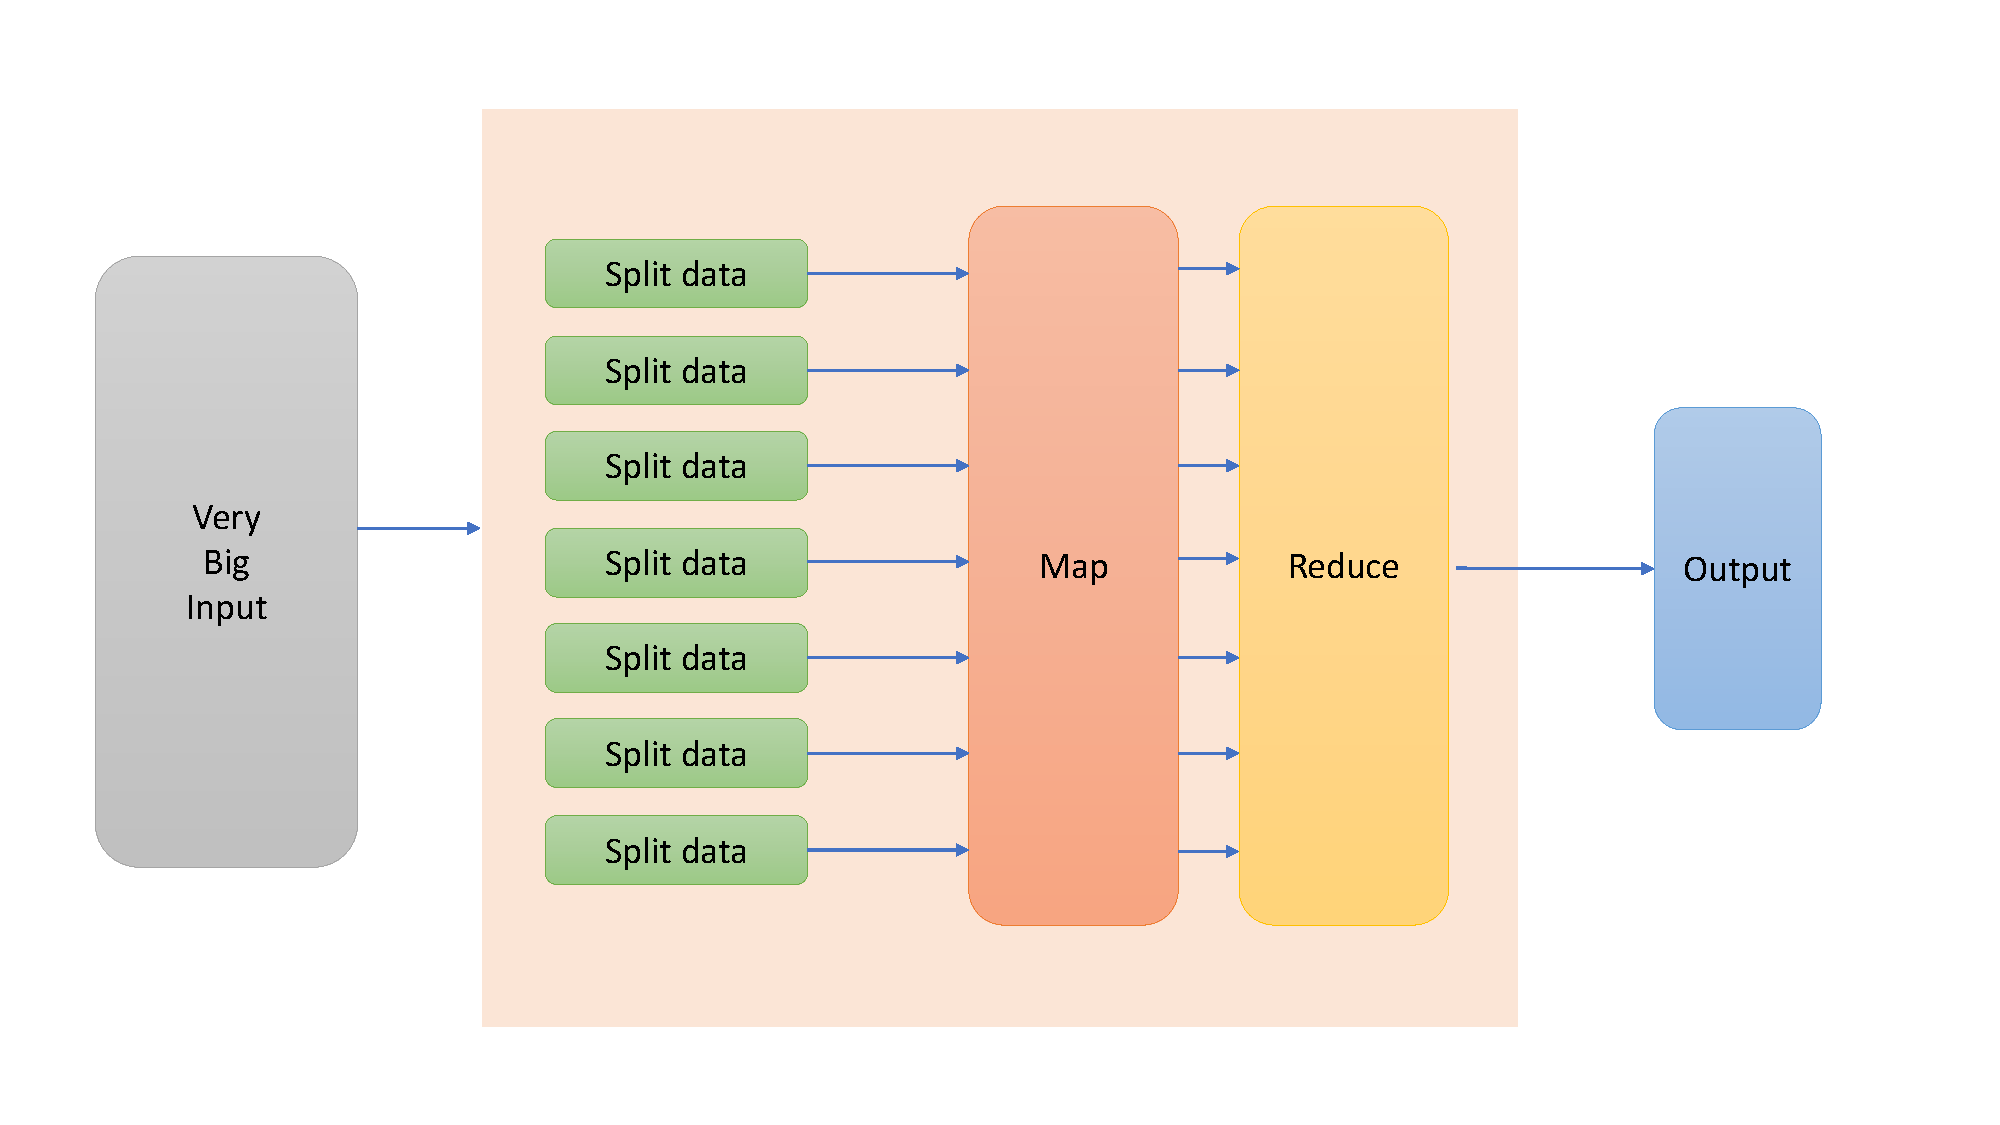
\includegraphics[width=\textwidth]{pics/mapReduce/overview}
	\caption{MapReduce Modell Übersicht}
\end{figure}


Um eine verteilte Berechnung und Verarbeitung zu vereinfachen, wird diese in zwei grobe Phasen aufgeteilt: Map und Reduce.
Für beide Phasen muss der Nutzer jeweils eine entsprechende Funktion definieren.
Der Input liegt als key/value Paare und vor und MapReduce produziert wiederum key/value Paare als Ergebnis.
In der Map Phase werden aus den gegeben key/value Paaren Zwischenwerte berechnet, welche wiederum als key/value Paare vorliegen. Diese werden anschließend gruppiert und in der Reduce Phase weiterbehandelt.
In der Reduce Phase werden dann die berechneten Zwischenwerte für gleiche keys zusammengefasst und aggregiert.

Beispiel:
Für eine Vielzahl von vorliegenden Dokumenten soll die Wortanzahl ermittelt werden.
Dann könnten die Map und Reduce Funktionen wie folgt aussehen:

\begin{lstlisting}[language=json,firstnumber=1]
map(String key, String value):
	// key: document name
	// value: document contents
	for each word w in value:
		EmitIntermediate(w, "1");

reduce(String key, Iterator values):
	// key: a word
	// values: a list of counts
	int result = 0;
	for each v in values:
		result += ParseInt(v);
	Emit(AsString(result));

\end{lstlisting}

Die Map function gibt also einfach jedes Wort plus ein Anzahl, in diesem Falle einfach 1 zurück.
Anschließend würde die Reduce Funktion alle zurückgebenen Anzahlen für jedes Wort summieren.



\section{Implementation}

Für das MapReduce Interface sind laut Paper (cite) verschiedene Umsetzungen möglich, die sich an den  Ausführungsumgebungen ausrichten.
Im Paper wird dann eine Umsetzung für eine damals typisch eingesetzte Environment vorgestellt.
Als Ausführungsumgebungen werden große Cluster (Anzahl 100-1000 Knoten) von Computern mit durchschnittlicher Rechenleistung und Hauptspeicher genannt.
Folgend wird beschrieben wie die Verteilung der Map und Reduce Funktion in dieser Umgebung von Google implementiert wurde.
Aufden Knoten läuft ein verteiltes Dateisystem (GFS), welches ein Zugriff auf Dateien über das Netzwerk ermöglicht, ein Knoten jedoch dabei diese Dateien wie lokate Dateien behandeln kann.
Der Nutzer übermittelt den MapReduce-Job an ein Scheduling System, welches dann die Ausführung koordiniert.


\subsection*{Vorbereitungen}
Ein Knoten übernimmt die Aufgabe des Masters, welcher dann die weitere Ausführung und das Scheduling übernimmt.
Der übermittle MapReduce-Job wird dann wie folgt in verschiedene Tasks aufgeteilt:
\begin{enumerate}
	\item
	Die Eingabedaten werden in M Parts gesplittet, pro Part wird später ein Map-Task ausgeführt.
	\item
	Die Reduce-Phase wird in R Reduce-Tasks aufgeteilt.
	Hierzu wird die Menge der möglichen Zwischenergebnisse
	durch eine Verteilungsfunktion in R Partitionen aufgeteilt.
\end{enumerate}
Diese Tasks werden den Workern dann dymamisch während der Ausführung zugeteilt.
Typische Zahlen sind: Z.B: M=200.000 R=4000, workers=2000

\subsection*{Ausführung der Map Phase}

In der Map Phase teilt der Master jedem freien Worker einen Map-Task zu.
Der Worker liest den zum Map-Task gehörenden Datenpart und führt darauf die Map-Funktion aus.
Hierbei werden (bis zu) R lokale Dateien (eine Datei pro Key) mit
Zwischenergebnissen lokal gespeichert.
Zum Schluss übermittelt der Worker den Speicherort der Zwischenergebnisse an den Master, damit diese später verteilt werden können.

\begin{figure}[H]
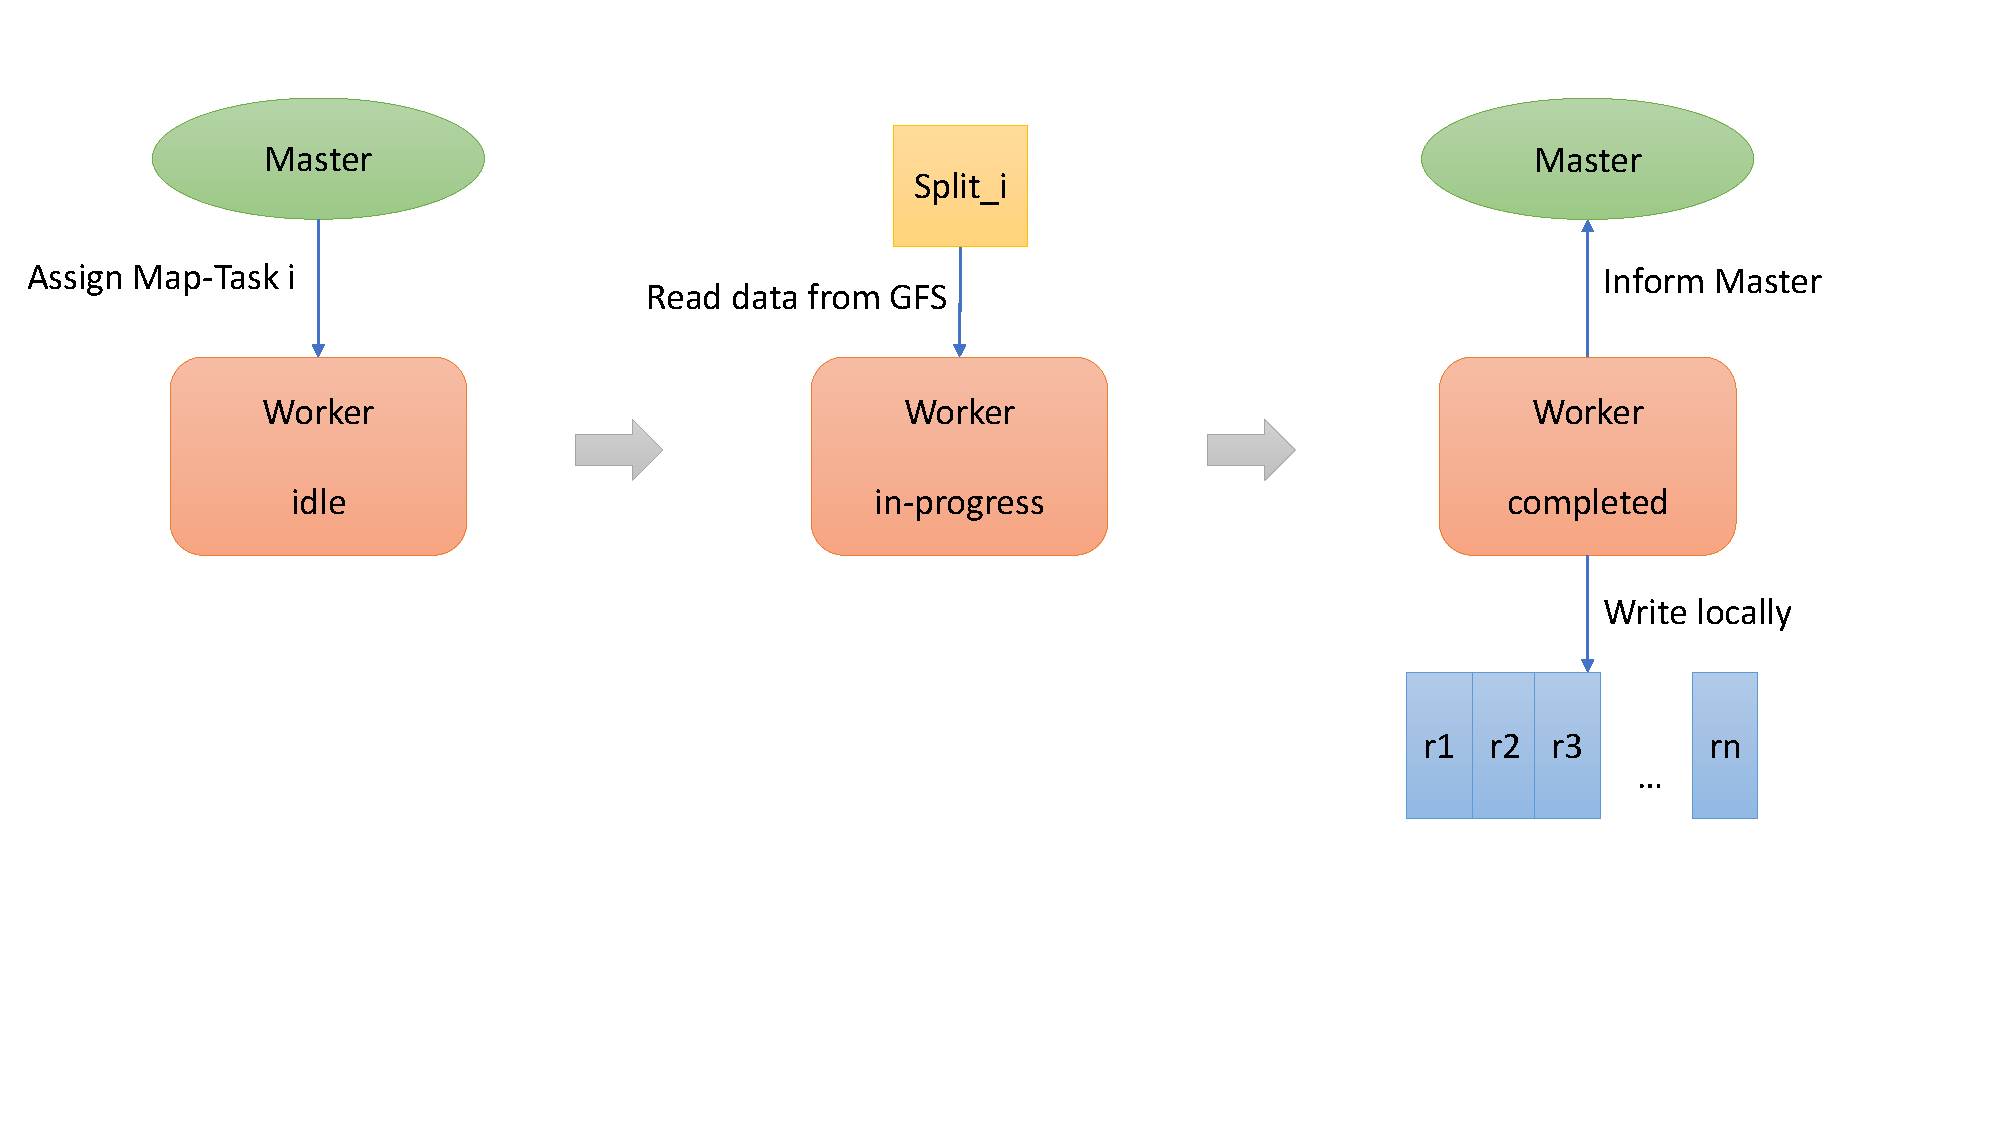
\includegraphics[width=\textwidth]{pics/mapReduce/mapassign}
	\caption{Ausführung eines Map tasks}
\end{figure}

\subsection*{Ausführung der Reduce Phase}

Der Master verteilt die Reduce-Tasks auf freie Worker und übermittelt dabei die Speicherorte der Zwischenergebnisse pro Key.
Dann liest der ausführende Worker die Zwischenergebnisse pro Key mittels RPC von den anderen Knoten, sortiert die Daten und wendet die vom User definierte Reduce-Funktion darauf an.
Anschließend wird ein Output-File mit dem Ergebnis ins verteilte Dateisystem geschrieben.


\begin{figure}[H]
	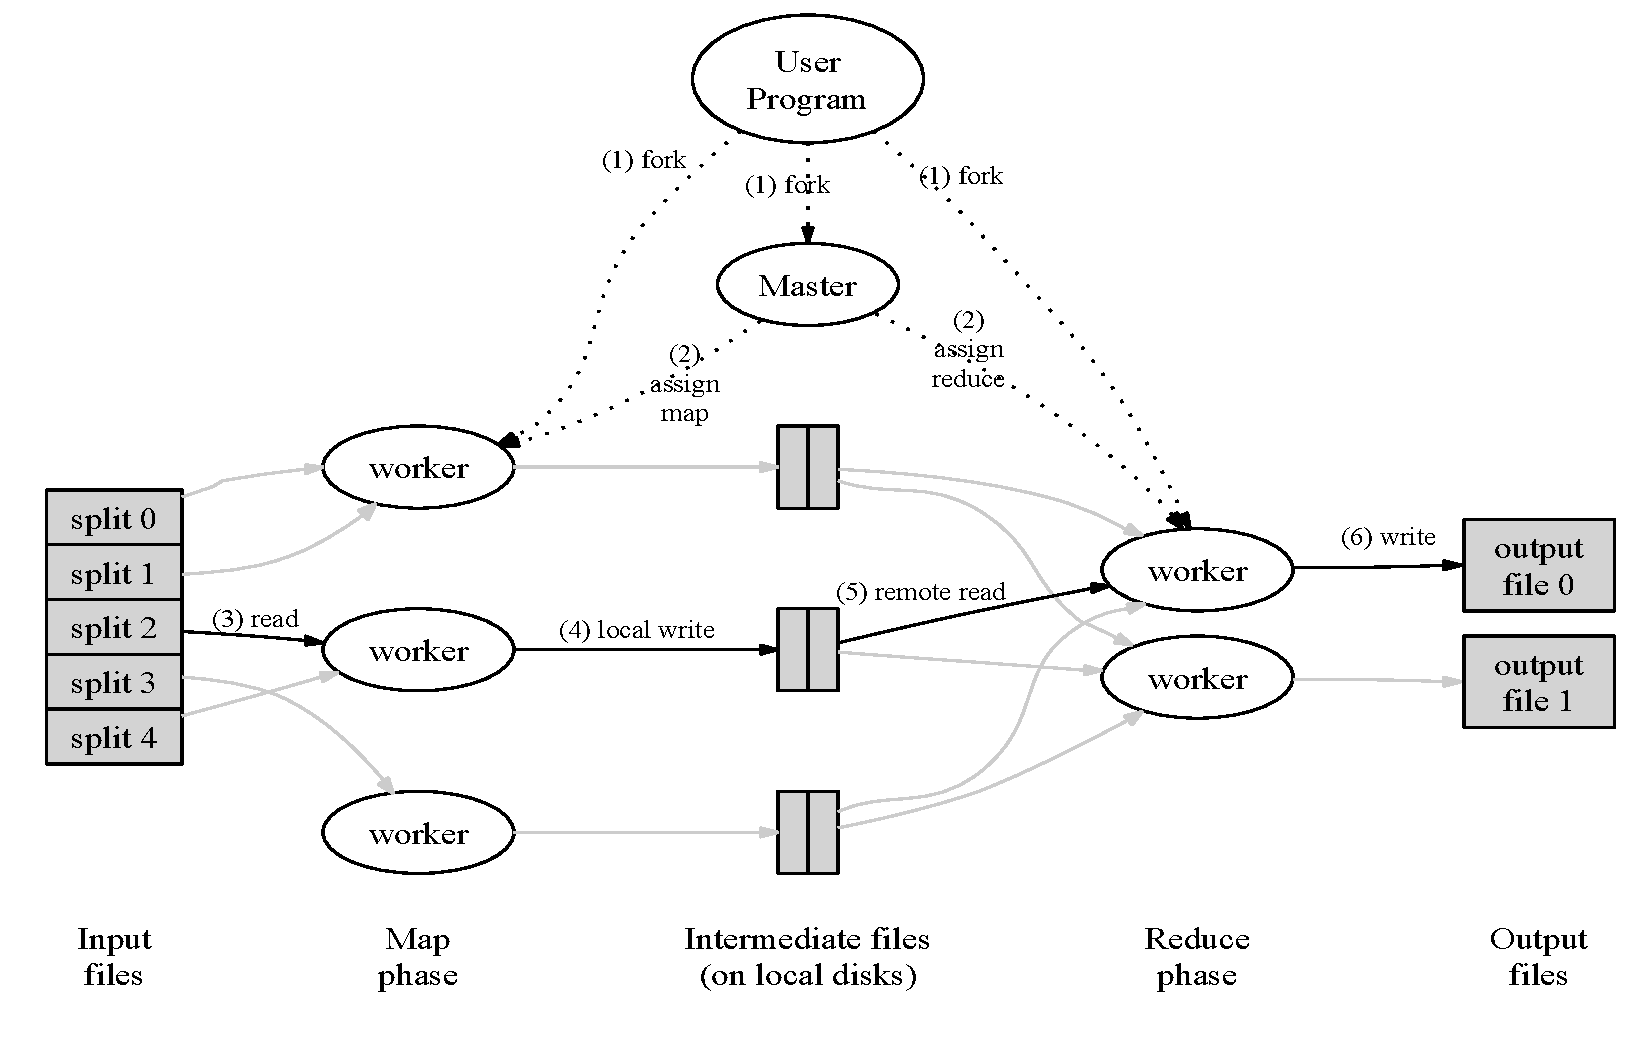
\includegraphics[width=\textwidth]{pics/mapReduce/mapreduce-osdi04e}
	\caption{Übersicht der gesament MapReduce Ausführungslogik}
\end{figure}


\subsection*{Fehlertoleranz}

Da MapReduce für den parallel Einsatzu auf vielen Knoten gedacht ist und einzelne Knoten ausfallen können, gibt es spezielle Fehlerfälle die betrachtet und behandelt werden.

Um ein Failure des Masterknotens aufzufangen, schreibt dieser periodisch Checkpoints vom derzeitigen Ausführungsstatus.
Tritt nun ein Fehler im Master auf, wird ein neuer Knoten als Master gestartet und die Ausführung vom letzten Checkpoint fortgeführt.

Jeder Workerknoten wird vom Master mittels Heartbeat periodisch auf Erreichbarkeit und Status abgefragt.
Wird ein ausgefallener Worker oder ein fehlerhafter Job erkannt, wird zwischen abgeschlossenen und nicht abgeschlossenen Job unterschieden.
Ein nicht abgeschlossener Map oder Reduce Task wird einfach auf einem anderen Worker neu gestartet.
Abgeschlossene Map Tasks werden auch erneut ausgeführt, da die Zwischenergebnisse lokal auf den Knoten liegen und diese entsprechend fehlen.
Abgeschlossene Reduce Tasks müssen nicht erneut ausgeführt werden, weil die Ergebnisse im verteilten Dateisystem gespeichert werden.


\section{Refinements}

Zur eigentlichen Ausführungslogik gibt es noch weitere Refinements, die die Ausführung optimieren.
\subsection*{Combiner}
In der Map Phase entstehen oftmals Wiederholungen von Zwischenergebnissen.
Im Wordcount Beispiel:
\begin{verbatim}
(foo bar bar bar) → (foo, 1) (bar, 1) (bar, 1) (bar, 1)
\end{verbatim}

Ein Worker kann nach Abschluss einen Map-Tasks die Zwischenergebnissen pro key mittels Combine Funktion zusammenfassen.
Z.B.
\begin{verbatim}
(foo, 1) (bar, 1) (bar, 1) (bar, 1) → (foo, 1) (bar, 3)
\end{verbatim}


\subsection*{Partitioning Function}

Die Nummer der Reduce-Tasks wird von Nutzer festgelegt.
Nun gibt es eine default Partitioning Function (hash(key) mod R),
welche die Zwischenergebnisse nach Keys den Reduce-Tasks zuordnet.
Durch die default PF werden meist gut verteilte Partitionen generiert,
allerdings kann der Nutzer auch eigene Verteilungsfunktionen definieren.

\subsection*{Datenlokalität}

Die Inputdaten werden im verteilten Dateisystem in Blöcke geteilt und repliziert auf verschiedenen Knoten gespeichert.
Da diese Blöcke später den MAP-Tasks zugeordnet sind, versucht der Master die Tasks so zu verteilen, dass die benötigten Blöcke auf den zugeordneten Knoten oder zumindest physisch in der Nähe liegen.
Hierdurch wird der Netzwerkdurchsatz während der Taskausführung reduziert und eine Ausbremsung verhindert.


\subsection*{Backup Tasks}

Einzelne, aufgrund Nebeneffekten sehr langsame Knoten, können den Gesamtprozess aufhalten, besonders wenn diese zum Ende eine Phase auftreten.
Um dies zu vermeiden, werden zum Ende einer MapReduce Phase Tasks welche noch nicht abgeschlossen sind, repliziert und auf mehren Knoten parallel ausgeführt.
Der erste abgeschlossene Task 'gewinnt' und langsame Knoten werden übergangen.


\section{Probleme und Nachteile von MapReduce}

MapReduce udn Spark (siehe chapter spark) ermöglichen die parallele und verteile Verarbeitung von riesigen Datenmengen.
Allerdings speichert und verarbeitet MapReduce alle Daten auf der Platte, während Spark durch eine in-memory Verarbeitung bis zu 100 mal schneller ist.
Auch bei iterativer Verarbeitung kann Spark durch die RDDs mehrere Operationen im Speicher ausführen, 
während MapReduce für jede Iterationen einen gesamten Durchlauf anstößt.
MapReduce zwingt den Nutzer die Verabeitung der Daten in eine Map- und eine Reduce-Funktion aufzuteilen, Spark bietet dem Nutzer hier viel mehr Komfort, weil zusätzliche Operationen möglich sind und eine High Level API anbietet. 

Zusätzlich bietet Spark eine Möglichkeit Streams zu verabeiten, was gerade in Hinsicht auf unseren Anwendungsfall, nämlich die Verarbeitung und live Analyse von Twitterdaten interessant ist. 


    \chapter{Spark}
\label{Spark}

\section[Spark und MapReduce]{\selectlanguage{ngerman}\rmfamily Spark
und MapReduce}
{\selectlanguage{ngerman}
Aufbauend auf der Vorstellung von MapReduce soll in diesem Abschnitt die
Software Spark beleuchtet werden. MapReduce ist ein Programmiermodell,
das auch bei Spark Anwendung findet. Allerdings bietet Spark weitaus
mehr Operationen. Die MapReduce-Referenzimplementierung ist Hadoop.
Spark integriert sich in das Hadoop-Ökosystem und wirkt dort als
Execution Engine.}

{\selectlanguage{ngerman}
Es wird ergänzt durch andere Komponenten von Hadoop wie dem
YARN-Ressourcen Manger, das verteilte Dateisystem HDFS,
Recovery-Mechanismen bei Ausfällen und Vorkehrungen zur
Datensicherheit.}

{\selectlanguage{ngerman}
Dabei nutzt Spark die persistente Storage von anderen und konzentriert
sich auf die Verarbeitung der verteilten Berechnungen im Speicher. Das
grundlegene Datenmodell soll hier besprochen werden, ebenso wie die
Architektur von Spark, die die Analysen ausführt und wie das im Spezialfall
Spark Streaming funktioniert.}

\section[RDDs]{\selectlanguage{ngerman}\rmfamily RDDs}
Wir beginnen mit der zentralen Datenstruktur, den RDDs. RDD steht für
Resilent Distributed Dataset. Die Grundidee hinter den RDDs ist es, die
Daten immutable (unveränderbar) vorzuhalten und einen festen Satz an
Operationen anzubieten. Diese Operationen erzeugen wiederum neue RDDs
oder bringen Analysen zu Ende. Spark soll zwei Ziele mit Hilfe der RDDs
erfüllen, nämlich Abstraktion von verteilten Arbeitsspeicherkonzepten
(distributed shared memory) und die Ausfalltoleranz.

Die RDDs werden im Hauptspeicher gehalten. Es geht nicht darum, wie
diese dauerhaft gespeichert werden können (persistiert werden).

Dadurch, dass es sich bei den RDDs um eine Abstraktion handelt, müssen
diese noch im konkreten Fall implementiert werden. Die RDDs sind nur
die Schnittstelle mit den definierten Operationen.

Für die Umsetzung betrachten wir im Folgenden noch verschiedene Dinge.
Anfangen werden wir bei dem Teil distributed im Namen der RDDs, nämlich
damit, wie die Verteilung bei Spark funktioniert.

\section[Funktionsweise Verteilung bei
Spark]{\selectlanguage{ngerman}\rmfamily Funktionsweise Verteilung bei
Spark}
Wie auch bei MapReduce werden bei Spark die gleichen Operationen auf
viele verschiedene Einzeldaten angewendet. Dabei erfolgt die Anwendung
der Operationen unabhängig voneinander für jedes einzelne Datum. Später
in der Berechnung werden dann einzelne Daten zusammengefügt. Damit
können die Daten verteilt werden. Spark bietet drei große Arten der
Partitionierung der Daten:

\begin{itemize}
\item Hash-Partitioning
\end{itemize}
Dabei entscheidet der Hashwert der Daten darüber, zu welcher Paritition
sie gehört. Vorteil ist, dass die Verteilung im Normalfall sehr
ausgeglichen zwischen Partitionen ist.

\begin{itemize}
\item Sort-Partitioning
\end{itemize}
Dabei werden die Daten sortiert und benachbarte Daten kommen in die
gleiche Partition. Vorteil ist es, dass s.g. Range-Anfragen schnell
beantwortet werden können, da die ähnlichen Daten benachbart sind.
Nachteilig ist, dass die Daten möglichweise sehr ungleich auf die
Partitionen verteilt sind.

\begin{itemize}
\item eigene Kontrolle über die Partitionierung
\end{itemize}
Der Programmierer eigener RDDs kann auch eigene Strategien zur
Partitionierung innerhalb der RDDs vorgeben. Dabei können auch schon
vorhandene Partitionierungen der Datenquellen weitergeführt werden.

Beispielhaft hierfür soll die Erstellung eines RDDs aus Daten von HDFS
(Hadoop Distributed Filesystem) gezeigt werden. Hier wird die eigene
Partitionierung so eingesetzt, dass die Daten in den RDDs auf den
gleichen Knoten liegen, wie die Daten im HDFS. Man spricht dann von
Datenlokalität.

Im HDFS sind die Daten in Blöcken partitioniert, die auf verschiedene
Rechner verteilt werden. Nun erfolgt ein 1:1 Mapping der Blöcke im HDFS
auf die Partitionen im \ RDD. So entsteht das HadoopRDD. Dieses
HadoopRDD kann dann mit den standartisierten RDD-Operationen ganz
normal weiterverarbeitet werden.

Liegen die Daten nicht schon verteilt vor, z.B. im einem verteilten
Dateisystem, so kann Spark sie auch automatisch verteilen. Dies erfolgt
beim Aufruf der Methode sc.parallize(). sc steht hier für SparkContext.
Dieses Objekt bietet viele Verwaltungsfunktionen an. 

\section[Lineage]{\selectlanguage{ngerman}\rmfamily Lineage}
\begin{figure}
\centering
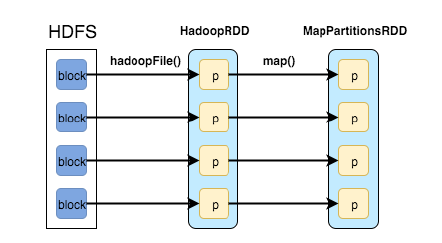
\includegraphics[width=\textwidth]{bilder/Seminartext-img1.png}
\caption{Erstellung RDD aus HDFS} 
\end{figure}
Wir haben im vorigen Abschnitt gesehen, wie Spark für die Verteilung das
Partitionieren (Sharding) vornimmt. Neben der Verteilung, die hier wie
im gesamten Projekt durch Scale-Out erfolgt, muss sich Spark auch um
Ausfalltoleranz kümmern. Durch die hohe Anzahl eingesetzter Rechner
steigt die Ausfallwahrscheinlichkeit stark an. Um die Erkennnung
ausgefallener Rechner kümmert sich der Ressourcenmanager und ebenso für
die Inbetriebnahme von Ersatzrechnern bzw. weiterer Rechner für höhere
Leistung.

Spark braucht allerdings einen Mechanismus, wie die Analyse fortgeführt
wird, wenn einer der Rechner ausgefallen ist. Zwei Dinge sind
beantworten: wie kommt man an die lokal gespeicherten Daten? Sie sind durch
den Ausfall nicht mehr zugreifbar und wie wird die Berechnung mit
diesen Daten fortgesetzt?

Die Antwort bei Spark ist erstaunlich einfach. Dies liegt daran, dass
die RDDs immutable sind. Dadurch kann das RDD nach erstmaliger
Fertigstellung nicht in einer unsauberen (dirty) Zustand kommen.
Mechanismen für ein UNDO teilweise fertiger Operationen sind also nicht
notwendig. Stattdessen wird nur ein REDO benötigt. Und um dieses Redo
geht es bei der sogenannten Data Lineage. \ Die Grundidee ist es, für
die RDDs die Herkunft, also die Entstehungsgeschichte aufzuzeichnen
bzw. im Voraus zu berechnen. Zur Erinnerung: das verloren gegangene RDD
ist durch eine Reihe von Transformationen von anderen RDDs aus den
ursprünglichen Eingabedaten entstanden. Fällt nun ein Knoten aus und
geht damit das RDD verloren, so können in der Lineage-Datenstruktur für
dieses RDD die Eltern-RDDs gefunden werden. Sofern diese noch vorliegen
(z.B. auf einem nicht-ausgefallenem Knoten), wird einfach die
aufgezeichnete Operation mit den Eltern-RDDs wiederholt. Sind diese
Eltern-RDDs ebenfalls nicht mehr vorhanden oder ausgefallen, so wird in
der Kette rekursiv durchgegangen. Am Ende stehen die orginalen
Eingabedaten. Das Konzept geht davon aus, dass diese Daten bereits
redundant vorliegen. Das ist auch der Fall, wenn z.B. HDFS genutzt wird
die Originaldaten hiervon geladen werden.

Diese Idee kann nun durch Checkpoints ergänzt werden. Unter einem
Checkpoint versteht man hier eine persistente Kopie von RDDs in einer
tieferen Lineage-Ebene. So muss bei einem Ausfall nur bis maximal zu
diesem RDD in dem Checkpoint zurückgegangen werden. Je länger die
Geschichte eines RDD ist, desto lohnender kann dieser Vorgang sein.
Dagegen spricht natürlich der erhöhte Speicherverbrauch.

Neben der Betrachtung auf RDD-Ebene lässt sich diese Betrachtung auch
auf Partitionsebene innerhalb des RDDs übertragen. Den eigentlich sind
die RDDs ja über mehrere Rechner verteilt (Scale-Out) und auf dem
Rechner liegen dann Partitionen verschiedener RDDs und meist nicht das
ganze RDD.

\section[Programmiermodell]{\selectlanguage{ngerman}\rmfamily
Programmiermodell}
Spark ist sowohl ein Framework, dass einfache Möglichkeiten für
verteilte Analysen bereitstellt, als auch eine Möglichkeit die so
erzeugten Analysen durchzuführen.

In diesem Abschnitt wird nochmal genauer auf das Programmiermodell
eingegangen. Die Daten werden mittels Scale-Out-Algorithmen verteilt
analysiert. Um möglichst hohe Parallelisierung zu erreichen, werden die
Daten in den meisten Fällen als unabhängig angenommen. Beispiele für
Eingabedaten sind Datenbanktabellen oder csv-Dateien.

Die einzelnen Einträge werden unabhängig voneinander vorverarbeitet.
Dies geschieht im Map-Schritt. Dann werden die Ergebnisse
zusammengefügt. Das passiert im Reduce-Schritt. So weit entspricht das
Vorgehen dem MapReduce-Programmiermodell. Spark erweitert es um einige
Operationen.

Dabei werden zwei Typen unterschieden: Aktionen, die aus einem RDD einen
konventionellen Datentyp, wie int, erzeugen. Der andere Typ sind
Transformationen, die aus RDDs wieder andere RDDs erzeugen. Dabei
werden neue RDDs erzeugt und nicht ursprünglichen RDDs verändert, denn
RDDs sind ja immutable.

Man könnte also von einem TransformAction-Programmiermodell als
Weiterentwicklung des MapReduce-Programmiermodells sprechen.

Zu den Transformationen gehören auch filter und flatMap. MapReduce
erweckt den Eindruck, dass es zumindest im Map-Schritt eine
1:1-Abbildung zwischen Elementen des einen RDDs zu Elementen des neuen
RDDs besteht. Natürlich lassen sich auch Elemente entfernen, die dann
im neuen RDD nicht mehr vorkommen (filter) und neue Elemente erzeugen. Dafür
wird eine Liste dieser Elemente als Transformationsergebnis für ein
Element erzeugt und statt map flatmap aufgerufen. Dabei werden alle
Listenelemente zu eigenen Elementen in dem neuen RDD.

Beispiele für Aktionen sind:

\begin{itemize}
\item count()
\item collect()
\item reduce()
\end{itemize}
Beispiele für Transformationen sind:

\begin{itemize}
\item map()
\item filter()
\item flatMap()
\item sample()
\item join()
\item sort()
\end{itemize}
Hinweis: Zur Zeit stellt Spark seine API von RDDs auf Dataframes um.
Diese haben deutlich erweiterte Möglichkeiten. Sie können mit ähnlichen
Operationen wie die von SQL bearbeitet werden.


\subsection{Beispielcode}

\subsubsection{Bekannte Wordcount}
\lstinputlisting[language=Java]{bilder/wordcount.scala}


\subsubsection{Approximation von PI}
\lstinputlisting[language=Java]{bilder/pi.scala}

Die Funktionsweise ist wie folgt: \ math.random liefert einen Wert
zwischen 0 und 1. Wir stellen uns einen Einheitskreis vor. Sein
Flächeninhalt ist$\pi r^2$, also bei $r=1$ $\pi$. Nun wird geprüft, ob die Koordinate (x,y) in
dem Einheitskreis liegt. Wenn dies der Fall ist, dann wird sie gezählt.
Der Anteil der Koordinaten, die in dem Einheitskreis liegen im
Vergleich zu der Gesamtzahl an Samples, entspricht gerade
$\frac{1}{4}\pi$ Der Faktor Vier
kommt daher, dass wir nur den ersten Quadraten des Einheitskreis
betrachten.

\section[Spark und Distributed Shared
Memory]{\selectlanguage{ngerman}\rmfamily Spark und Distributed Shared
Memory}
Am Anfang haben wir als ein Ziel von Spark die Abstraktion für
Distributed Shared Memory beschrieben. Das wollen wir nun nochmal
aufgreifen und beide vergleichen. Dadurch, dass die Operationen
gegenüber der Distributed Shared Memory eingeschränkt werden, nämlich
insbesondere Veränderungen nur bei gleichzeitiger Kopie des RDDs
vorgenommen werden können, entfallen viele Aufgaben. Distributed Shared
Memory funktioniert wie verteilter Arbeitsspeicher, d.h. die einzelnen
Rechner können mehr oder weniger unreguliert Lese- und
Schreiboperationen vornehmen. Damit das nicht im Chaos endet, müssen
sie sich Protokolle zur Synchronisation nutzen. 

Betrachten wir einige Aufgaben genauer:


\begin{itemize}
\item Konsistenz der Daten sicherstellen
\end{itemize}
Ist bei RDDs nicht notwendig, da die RDDs immutable sind. Es muss nur
überwacht werden, ob das RDD vollständig erzeugt wurde. Dadurch wird der
ganze Transformationsvorgang atomar. Bei Distributed Shared Memory ist
das nicht so. Da sind zusammengehörige Schreiboperationen nicht atomar,
d.h. es ist durchaus möglich, dass der erste Teil der
Schreiboperationen bereits umgesetzt wurde (z.B. Kontostand bei einer
Überweisung verringern), der zweite Teil aber nicht (z.B. Kontostand
beim Empfänger erhöhen). Deshalb muss die Anwendung hier ein spezielles
Protokoll zwischen den Knoten einführen.

\begin{itemize}
\item Fault Recovery
\end{itemize}
Kann bei RDDs durch Lineage vergleichsweise einfach vorgenommen werden.
Bei Distributed Shared Memory ist wieder ein kompliziertes Protokoll
notwendig. Checkpoints sichern die Daten. Da die Konsistenz aber nicht
notwendigerweise gegeben ist, braucht es Rollback-Vorgänge. 

Eindeutiger Nachteil der RDDs ist ihr schlechter Umgang mit
feingranualaren Schreibevorgänge, d.h wenn nur wenige Elemente eines
RDDs geändert werden sollen. Distributed Shared Memory liegt hier
eindeutig vorne, da alle Operationen feingranular erfolgen können.

\section[Spark{}-Architektur]{\selectlanguage{ngerman}\rmfamily
Spark-Architektur}
Hauptaugenmerk in diesem Abschnitt soll auf der Berechnung der Job
Stages liegen. Mit Hilfe der Transformationen und Aktionen lassen sich
komplexe Abfolgen von Operationen auf unterschiedlichen RDDs und auch
in Kombination dieser RDDs erzeugen. Während die Transformationen für
alle Partitionen parallel ausgeführt werden können, müssen die parallel
erfolgenden Operationen durch Spark erst berechnet werden.

Dazu werden die komplexen Operationsfolgen in Stages unterteilt. Sie
entsprechen den Knoten in einem DAG (einem azyklischen Graphen).
Dadurch entsteht eine partielle Ordnung der Stages. Stehen zwei Stages
weder in einer Vor- noch in einer Nacheinander-Beziehung, so können sie
parallel berechnet werden, sofern ihre Eltern-RDDs bereits berechnet
wurden. 

Ein entscheidender Unterschied stellen hier die Operationen da. Sind die
Operationen Joins oder groupByKey, so müssen alle daran beteiligten
RDDs vollständig berechnet sein, damit die Operation ausgeführt werden
kann. Man spricht dann von einer wide dependency. D.h. bei der
Ausführung muss das erste RDD auf die anderen RDDs warten. Andere
Operation wie map, union, join mit co-partitionierten Input oder filter
brauchen das nicht. Sie liegen innerhalb eines Stages in einer Abfolge.
Man spricht hier von narrow dependencies.

\begin{figure}
\centering
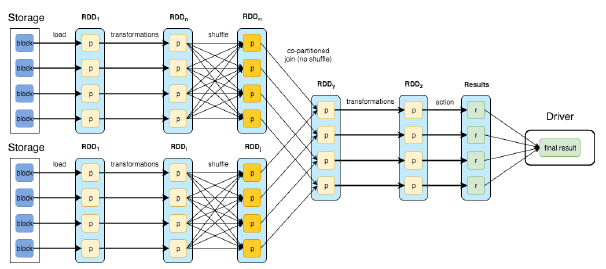
\includegraphics[width=\textwidth]{bilder/Seminartext-img2.png}
\caption{Spark Stages}
\end{figure}

\bigskip

\subsection[Durchlauf durch
Komponenten]{\selectlanguage{ngerman}\rmfamily Durchlauf durch
Komponenten}
Betrachten wir nun Einbindung der Job-Stage-Berechnung in die
Architektur. Alles fängt mit den RDDs an, die inkl. ihrer Lineage aus
dem Javacode ermittelt werden. Sie werden als DAG in den DAGScheduler
eingegeben. Dieser berechnet die möglichen Jobstages und ermittelt
daraus TaskSets für die einzelnen Rechnenknoten. Er gibt sie an den
Clustermanager weiter. Dieser verteilt sie dann an geeignete Knoten. In
diesen Knoten, den Executors, werden diese dann in Threads ausgeführt. 

\begin{figure}
\centering
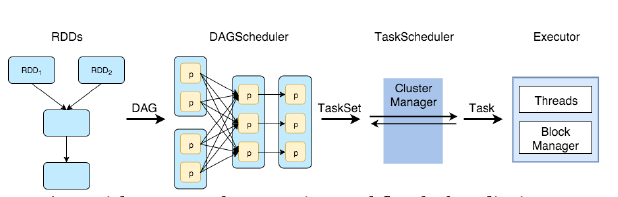
\includegraphics[width=\textwidth]{bilder/Seminartext-img3.png}
\caption{Spark Architektur}
\end{figure}

\bigskip

\section[Vor{}- und Nachteile von
Spark]{\selectlanguage{ngerman}\rmfamily Vor- und Nachteile von Spark}
Fassen wir nochmal die Vorteile und Nachteile von Spark zusammen.
Entscheidend ist die Art von Programm, das ausgeführt werden soll.
Jenachdem ist Spark besser oder weniger gut geeignet.

Schlecht geeignete Programme sind Programme mit vielen asynchronen,
feingranularen Updates auf einem gemeinsamen Zustand. Dies würde zu
einer Explosion der Anzahl von RDDs führen. Beispiele hierfür sind
Web-Anwendungen und inkrementelle Web-Crawler. Alternativen wären
RAMCloud, Percolator und Piccolo.

Gut geeignete Programme führen Bulk Writes auf vielen Daten aus.
Insbesondere dann, wenn Datenlokalität ausgenutzt werden kann, ist
Spark gut geeignet. Spark punktet dann mit effizienter Fault Tolerance
durch Lineage und Ausgleich von langsamen Knoten, da kein Rollback
notwendig ist.

\section[Funktionsweise Spark
Streaming]{\selectlanguage{ngerman}\rmfamily Funktionsweise Spark
Streaming}
Als letztes wollen wir noch die Funktionsweise einer Variante von Spark
anschauen, nämlich Spark Streaming. Wenn man nicht auf periodisch
ausgeführte Analysen warten möchte, sondern gewissermaßen live auf
Ergebnisse zugreifen möchte, kann Spark Streaming eingesetzt werden.

Die Eingabedaten kommen dabei als kontinuierlicher Stream. Sie werden in
Microbatches zerlegt, d.h. es werden z.B. die Daten einer Sekunde
zwischengespeichert. Dann wird ein herkömmlicher Spark-Job auf dem
Batch ausgeführt. Dies wird kontinuierlich für die einkommenden Streams
gemacht. Spark nennt dieses Vorgehen D-Streams. Es ist ein Denkmodell
dafür, dass einkommende Einträge als Microbatches in einem RDD
gespeichert werden. Auf diesem werden dann parallel deterministische
Operationen ausgeführt, analog wie bei der Batch-Analyse. Ein D-Stream
ist also eine Folge von Datensets. Es ist keine komplexe
Synchronisation der einzelnen Knoten notwendig. Sie operieren
unabhängig voneinander und bekommen ihre Aufgaben aus dem DAGScheduler
vorgegeben. Sie greifen nicht auf gemeinsamen Speicher schreibend zu.
\ Ausfälle von Knoten sowie zu langsame Knoten lassen sich genau wie
sonst auch beheben. 

\begin{figure}
\centering
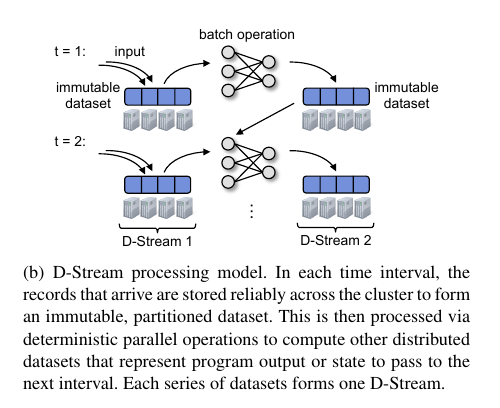
\includegraphics[width=\textwidth]{bilder/Seminartext-img4.png}
\caption{Sparks DStreams}
\end{figure}
\subsection[alternatives, nicht verwendetes
Denkmodell]{\selectlanguage{ngerman}\rmfamily alternatives, nicht
verwendetes Denkmodell}
Ein alternatives Modell wäre der Continuous Operator. Dabei haben die
Nodes einen inneren Zustand, ggfs. gibt es einen dezidierten
gemeinsamen Zustand. Ausfalltoleranz kann dann mit einem
Synchronisationsprotokoll erreicht werden, das Replikation vorsieht.
Schwieriger ist hier die Recovery. Da die zusammenhängenden
Schreiboperationen nicht atomar ausgeführt werden, braucht man wie bei
bei Distributed Shared Memory Rollback und weitere Mechansimen.

Allerdings können hiermit auch komplexere Berechnungen vorgenommen
werden. Es gibt die künstlichen Microbatches-Grenzen nicht.
Dementsprechend sind z.B. Rolling-Windows einfacher. 
	\colorlet{punct}{red!60!black}
\definecolor{background}{HTML}{EEEEEE}
\definecolor{delim}{RGB}{20,105,176}
\colorlet{numb}{magenta!60!black}

\lstdefinelanguage{json}{
    basicstyle=\normalfont\ttfamily,
    numbers=left,
    numberstyle=\scriptsize,
    stepnumber=1,
    numbersep=8pt,
    showstringspaces=false,
    breaklines=true,
    frame=lines,
    backgroundcolor=\color{background},
    literate=
      {0}{{{\color{numb}0}}}{1}
      {1}{{{\color{numb}1}}}{1}
      {2}{{{\color{numb}2}}}{1}
      {3}{{{\color{numb}3}}}{1}
      {4}{{{\color{numb}4}}}{1}
      {5}{{{\color{numb}5}}}{1}
      {6}{{{\color{numb}6}}}{1}
      {7}{{{\color{numb}7}}}{1}
      {8}{{{\color{numb}8}}}{1}
      {9}{{{\color{numb}9}}}{1}
      {:}{{{\color{punct}{:}}}}{1}
      {,}{{{\color{punct}{,}}}}{1}
      {\{}{{{\color{delim}{\{}}}}{1}
      {\}}{{{\color{delim}{\}}}}}{1}
      {[}{{{\color{delim}{[}}}}{1}
      {]}{{{\color{delim}{]}}}}{1},
}

\chapter{Search Engine}
Die Twitter-Klon Applikation soll mit einer Suchfunktion erweitert werden. Diese Suchfunktion wird mit einem Such-Service umgesetzt, der auf der Elasticsearch-Engine basiert. Elasticsearch setzt auf Apache Lucene auf, einer in Java geschriebenen Bibliothek für die Volltextsuche. Es ist open-source, dokumentenorientiert, in Java geschrieben und lässt sich über einen REST-API ansprechen. Damit ist es ein guter Kandidat für unser Use-Case.

\section{Zielsetzung}
Das Ziel des Suchservices ist die Ausgabe von \textit{best-match} Ranglisten über eine Tweets-Sammlung zu erstellen, indem man nach bestimmten Benutzern, Tags und Freitexteingaben sucht. Als Erweiterung der Suchfunktion wird ein Text-Vervollständigung Feature erstellt, das beim Suchen nach Tweets passende Vorschläge liefert. Und zum Schluss sollen ausgewählte Datensätze, mit Hilfe eines Analyse- und Visualisierungstools, auf der Homepage als eine Grafik angezeigt werden. 

\section{Vorgehen}
Zuerst wird eine \textit{Elasticsearch-Service} Architektur angefertigt. Diese stellt nur ein Teil der \textit{Twitter-Klon} Umsetzung und behandelt die Kommunikation zwischen \textit{Elasticsearch}, \textit{Elasticsearch-Service} wie den \textit{Kafka-Topics}. Nachfolgend wird Elasticsearch entsprechend der \textit{Twitter-Klone} Applikation konfiguriert und für die Datenaufnahmen vorbereitet. Infolgedessen wird der Such-Service implementiert, der \textit{Elasticsearch} mit den \textit{Kafka-Topics} verbindet und für den Datenaustausch zuständig ist. Anschließend werden Datenvisualisierungen mit Hilfe von \textit{Kibana} angefertigt. Zum Schluss wird der Elasticsearch Abschnitt mit einem Fazit beendet.

\section{Service Design}
Der komplette Nachrichtenaustauch der \textit{Twitter-Klon} Applikation wird mit einem skalierbaren und performanten Messaging-Service umgesetzt, nämlich \textit{Apache Kafka}. Dieser, bietet die Möglichkeit, mit Hilfe der Nachrichten-Topics den Overhead an Kommunikation zwischen den Services zu verringern, die Services von einander zu entkoppeln und die Daten parallel zu verarbeiten.
Diese Eigenschaft ermöglicht das Entkoppeln des Such-Service‘es von dem Restsystem, sodass die Suche unabhängig von den Schnittstellen der heterogenen Klienten bedient werden kann. 
Dafür wurden drei Topics erstellt und ein Datenformat vereinbart, das langfristig alle unsere Wünsche abdecken soll. Die Such-Service Use-Cases sind in drei Gruppen eingeteilt, die mit Hilfe von drei Kafka-Topics realisiert wurden: Neue Dokumente indexieren/abspeichern, Anfragen empfangen und Anfragen beantworten.
%\captionsetup{justification = raggedright,singlelinecheck = false}
\begin{figure}[htbp!]
	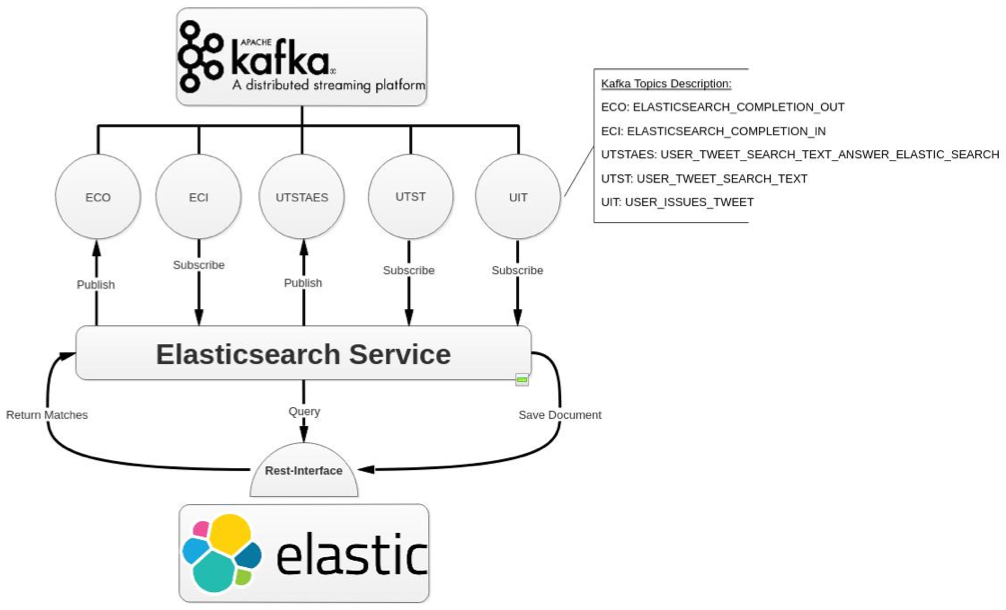
\includegraphics[scale=0.8]{material/architecture/Elasticsearch.png}
	\caption{Elasticsearch Service Architectur}
	\label{fig:ESA}
\end{figure}

Der Such-Service meldet sich an den entsprechenden Kafka-Topics an, öffnet ein Datenstrom und empfängt Nachrichten mit den Speicher-, Suchkriterien, sowie der dazugehörigen Benutzerkennung. Um den Speicherplatz optimal zu nutzen, werden aus der Nachricht nur für die Suche relevante Felder ausgelesen und an die Elasticsearch REST-Schnittstelle weitergeleitet, wie z.B. der Text, die Benutzerkennung, die Tags und der Zeitstempel.  

Das Verschicken der Nachrichten über unsere Applikation durchläuft den \textit{UIT} Topic, dieser bietet jedem Abonnenten den Zugriff auf die neu eingetroffenen Mitteilungen. Der Elasticsearch-Suchservice ist einer der bestehenden Abonnenten des \textit{UIT} Topics und bereitet die neu eingetroffenen Nachrichten für die Weiterleitung und das Speichern des Inhalts in Elasticsearch. Die, mit Metainformation bestückten, Nachrichten laufen eine Transformation durch wie Filterung, Umbenennung und Umstrukturierung, um der Elasticsearch erwarteten Datenstruktur zu entsprechen und Speicherplatz zu sparen. 

Für die Suchfunktion werden die Topics \textit{UTST} und \textit{UTSTAES} genutzt. Über den \textit{UTST} werden Suchanfragen entgegengenommen und in eine Elasticsearch-Rest-Anfrage umgeformt. Die Suchanfrage kann von dem Suchservice auf verschiedene Weise durchgeführt werden. Zum Beispiel durch eine Term-, Bollean-, Match-, Multimatch- und Match-Phrase- Suche. Jede Abfrageart, kann im bestimmten Fällen vorteilhaft ausgenutzt werden und kann Fallspezifisch eingesetzt werden. 
Das Suchergebnis wird anschließend als eine sortierte Identifikationsliste zu enthaltenen Nachrichten auf dem \textit{UTSTAES} Topic hinterlegt. Damit wäre die Suche beendet und das weitere Geschehen des Suchergebnisses den \textit{UTSTAES} Abonnenten überlassen.

Die Suchvervollständigung verhält sich ähnlich der Suchfunktion. Der Suchservice kommuniziert über die Topics \textit{ECI} und \textit{ECO}, die vervollständigung Anfragen für die Benutzereingabe publizieren und mögliche Eingabewünsche entgegennehmen. Die Eingabewünsche könne mit Hilfe der Elasticsearch Vervollständigung oder durch die nGrams-Implementation umgesetzt werden. Diese Ansätze sind in der Granularität, Umsetzung, Laufzeit und Speicherbedarf unterschiedlich und könne Fallabhängig ausgetauscht werden. 


\section{Elasticsearch Konfiguration}
Elasticsearch funktioniert \textit{out of the box}, das heißt, man muss den Service nur starten und das Indexieren, wie das Suchen der Dokumente funktioniert reibungslos. Im Gegensatz zu den relationalen Datenbanken ist eine Schema Definition für Elasticsearch nicht notwendig. Obwohl ein Schema nicht gefordert ist, ist es höchst ratsam dieses zu deferieren, denn das \textit{Type-Matching} der Felder wird ansonsten nach dem \textit{Best Guess} Prinzip erstellt und kann unter umstanden zum unerwünschten Verhalten führen.

\subsection{Index Settings}
Die \textit{out of the box} Fähigkeit von Elasticsearch ist toll zum Ausprobieren, jedoch ist es für den Betrieb ungeeignet, da die Einstellungen für die bestmögliche Skalierung von Elasticsearch, wie das Durchsuchen der Texte immer von der Domäne abhängt. Falsche oder keine Anpassung, kann die Skalierungsmöglichkeiten von Elasticsearch drastisch senken und damit den Betrieb unerwartet unterbrechen. Des Weiteren ist die Anpassung der Textvorverarbeitung eine Kernaufgabe jeder Such-Engine, dementsprechend sollte man sich besonders sorgfältig um diese Aufgabe kümmern, sodass alle relevanten Ergebnisse ermittelt und in einer passenden Ordnung dem Nutzer vorgelegt werden können.

\subsection{Sharding \& Replication}
Zuerst wird der Elasticsearch Index auf Shards und Replicas aufgeteilt. Damit enthält ein Shard eine Teilinformation oder ein Replikat der Teilinformation des Indexes, der auf unterschiedliche Hardware aufgeteilt werden kann. Obwohl die Verschiebung des Shards Knotenübergreifend realisiert werden kann, kann dieser nicht in zwei neue Shards gespalten werden, wenn die Hardware an ihre Grenzen stößt. Damit ist ein Shard die Skalierungseinheit des Indexes und muss sorgfältig gewählt werden. Der uns gegebene Elasticsearch Cluster arbeitet nur auf einem Knoten, dementsprechend ist der Skalierungsfaktor von fünf genug um zukunftssicher den Index bis auf fünf weitere Knoten aufteilen zu können. Der Replikationsfaktor beschreibt wie viele Replikate für einen Shard erstellt werden. Für eine Einstellung aus fünf Shards und einem Replikat entsteht eine Gesamtdatenmenge von 10 Shards. Daraus folgt ein immenser Anstieg an Speicherverbrauch für jeden nächsten Replikat eines Shardes. Die Replikate bieten im Gegensatz die Ausfallsicherheit und die Performance Steigerung der Lesezugriffe. Da die Performance und die Ausfallsicherheit für jeder skalierbare Applikation Kernkriterien sind, kann Elasticsearch diese bei Bedarf im laufenden Betrieb durch neue Replikate stärken. In unserem Fall steht nur einen Knoten zur Verfügung, dementsprechend folgt kein Anstieg der Performance wie Ausfallsicherheit mit Hilfe der Replikation.
% Bild  mit Reploikation der Shards und Replikas auf Knoten.
\\\\
\textbf{Initiale Index Einstellungen}
\begin{lstlisting}[language=json,firstnumber=1]
{
  "twitterindex": {
    "settings": {
      "index": {
        "number_of_shards": "2",
        "number_of_replicas": "0",
        "refresh_interval": "1s",
        "provided_name": "twitterindex",
        "creation_date": "1529674155106",
        ...
        "uuid": "wOHQnu5GQjOs7iP-Cv-_MQ",
        "version": {
          "created": "6020399"
        }
      }
    }
  }
}
\end{lstlisting}

\subsection{Textvorverarbeitung}
Als nächstes wird der Textvorverarbeitungsprozess definiert. Unter dem Schlüssel \textit{Analyzer} wird ein \textit{Custom Analyzer} und die dazugehörigen Vorverarbeitungsschritte erstellt. Dieser wird innerhalb Elasticsearch aufbewahrt und mit Funktionalität belegt. Der Analyzer zerlegt den Text mit dem \textit{Partial Word Tokenizer} in Tokens nach einem bestimmten Muster, nämlich nach einem Leerzeichen, nach einem Großbuchstaben Anfang und nach einer Zahl.
Dieser Zerlegungsschritt erfüllt die gegebenen Anforderungen, könnte aber auf Kosten des Speicherplatzes durch den mächtigeren \textit{Edge NGram Tokenizer} ausgetauscht werden. Nachfolgend laufen die Tokens eine Transformationskette durch. Zuerst werden die Tokens in Kleinbuchstaben umgewandelt, auf den Wortstamm zurückgeführt und Worte mit geringen Informationsgehalt, sowie verboten Worte entfernt. Zuletzt werden die Worte mit ähnlicher Bedeutung wie \textit{Universität Hamburg} und \textit{UHH} in Synonymlisten zusammengefasst und als gleichgültig behandelt. 
\\\\
\textbf{Analyzer}
\begin{lstlisting}[language=json,firstnumber=1]
"analyzer": {
...
  "my_analyzer": {
    "filter": [
      "my_tokenizer",
      "lowercase",
      "my_stemmer",
      "english_possessive_stemmer",
      "my_stop",
      "my_synonym"
    ],
    "type": "custom",
    "tokenizer": "standard"
  },
...
}
\end{lstlisting}

\subsection{Data Mapping}
Zuletzt braucht Elasticsearch ein Datenschema, um die automatische Fehleinschätzung des Mappings zu vermeiden. 
Elasticsearch baut einen Suchindex auf, der Dokumentenbasiert in einem JSON Format abgespeichert wird. Das Mapping garantiert eine Typenzusicherung wie das Format, der zu speichernden Felder und Dokumente. Zum Beispiel das Datumformat, das Regionsunabhängig vor dem Abspeichern von Elasticsearch normalisiert wird oder das Textfeld, das man mit bestimmten Eigenschaften und Funktionen anreichert, um das gewünschte Verhalten zu realisieren. 
Der Text, kann als \textit{Keyword} abgespeichert werden, das Eins-zu-eins durchsucht wird oder ein \textit{Text}, das mit Hilfe der Volltextsuche komplexen Suchkriterien umsetzen kann.
Das Elasticsearch Mapping für den Twitter-Klon definiert ein Dokumentenformat mit sieben Felder: id, message, tags, users, timeStamp, userLocation und userLocationCompletion. Für die Suche sind die Felder \textit{message}, \textit{tags} und \textit{use} relevant, diese werden vom Type \textit{Keyword} und \textit{Text} gespeichert. Das Feld \textit{timeStamp} wird auf ein \textit{Long} projiziert und für die Datenvisualisierung mit Kibana genutzt, um die wöchentlichen Trends anzuzeigen. Das Feld \textit{userLocation} hält die vom Benutzer eingetragene Standort, der mit der Textvervollständigungsinformation von Elasticsearch angereichert und durch das Feld \textit{userLocationCompletion} beschrieben. Zum Vergleich wird das Feld \textit{userLocation}  zusätzlich mit dem \textit{nGram Analyzer} belegt, um die Text-Verfollständigung von Elasticsearch mit der \textit{nGram} Methode vergleichen zu können.  
\\\\
\textbf{Mapping}
\begin{lstlisting}[language=json,firstnumber=1]
"userLocation": {
  "type": "text",
  "analyzer": "nGram_analyzer",
  "search_analyzer": "nGram_search_analyzer"
},
"userLocationCompletion": {
  "type": "completion",
  "analyzer": "simple",
  "preserve_separators": true,
  "preserve_position_increments": true,
  "max_input_length": 50
},
\end{lstlisting}


\section{Search Service}
Die Implementation des Such Service wird mit Java und Spring realisiert. Spring ist ein weit verbreitetes und etabliertes Enterprise Framework für Java. Dieses besitz eine große Palette an Werkzeigen, die das Arbeiten in einer heterogenen Umgebung stark vereinfachen. Daher eignet sich Spring besonders gut für unseren Anwendungsfall. Für den Nachrichtenaustausch zwischen Apache Kafka, Elasticsearch und dem Suchservice wird, die von Spring entwickelte \textit{Spring for Apache Kafka} und die von Elasticsearch angebotene \textit{Elasticsaerch Rest Client} Bibliotheken genutzt.
Die interne Logik des Suchservices wird von den Java Beans umgesetzt, die im Springkontext auf dem Apache Tomcat Application Server ausgeführt werden und die gewünschte Such-Funktionalität umsetzen.

\subsection{Such-Interface}
Um die Kommunikation und Fähigkeiten des Such Services übersichtlich zu gestalten, wird ein Interface mit den gewünschten Anfragen erstellt und anschließend implementiert. 

\begin{enumerate}
	\item über die Tags
	\item über die referenzierten Benutzer
	\item über angegebenen Standortnamen mit der Textvervollständigung
	\item über die Term-Suche auf den Tweet-Text
	\item über die Volltextsuche auf den Tweet-Text
	\item über den Text wie den Benutzet Standortnamen
	\item über einen Zeitraum
	\item über einen Zeitraum mit Benutzer und Tag Präferenz 
\end{enumerate}

\subsection{Such-Implementation}
Elasticsearch bietet eine JSON-ähnliche domänenspezifische Sprache, mit der man Abfragen ausführen kann. Dies wird als \textit{DSL Query} bezeichnet. Die Abfragesprache ist ziemlich umfassend und bietet komplexe Filter und Aggregation Möglichkeiten. Die Anfragen des Suchservices sind ausgelegt die wichtigsten Anfragemöglichkeiten von Elasticsearch darzustellen. Es werden \textit{term}, \textit{match}, \textit{multi match}, \textit{match phrase}, \textit{bool}, \textit{compleation} und \textit{aggregation} Anfragen behandelt. 
\\\\
\textbf{Suchen nach Tags}
\begin{lstlisting}[language=json,firstnumber=1]
{
  "query": {
    "terms": {
      "tags.keyword": "?"
         }
    }
}
\end{lstlisting}

\textbf{Suche nach Referenzierten Benutzer}
\begin{lstlisting}[language=json,firstnumber=1]
{
  "query": {
    "terms": {
      "users.keyword": "?"
    }
  }
}
\end{lstlisting}

Die Tag- und Benutzersuche wird mit der Term-Suche umgesetzt, diese sucht nach Dokumenten, die genau, die im angegebenen Feld angegebenen Begriffe enthalten. Die Tweets werden entsprechend den TF/IDF Relevanz sortiert und präsentiert.  
\\\\
\textbf{Textvervollständigung nach Standortnamen}
\begin{lstlisting}[language=json,firstnumber=1]
{
  "suggest": {
    "location_suggest": {
      "prefix": "?",
      "completion": {
        "field": "userLocationCompletion",
        "fuzzy": {
          "fuzziness": 1
        }
      }
    }
  }
}
\end{lstlisting}
Der Textvervollständigung bietet Funktionen zur automatischen Vervollständigung. Es werden Vorschläge wehrend des Tippens einer Anfrage getätigt und führt schneller zu relevanten Ergebnissen. Durch die zusätzliche \textit{fuzzy} Eigenschaft der Abfrage werden zusätzlich Tippfehler abgefangen um die Suche den Nutzer angenehmer zu gestalten.
\\\\
\textbf{Term-Suche auf den Tweet-Text}
\begin{lstlisting}[language=json,firstnumber=1]
{
  "query": {
    "match": {
      "message": "?"
    }
  }
}
\end{lstlisting}

\textbf{Volltextsuche auf den Tweet-Text}
\begin{lstlisting}[language=json,firstnumber=1]
{
  "query": {
    "match_phrase": {
      "message": {
        "query": "?",
        "slop": 1
      }
    }
  }
}
\end{lstlisting}

Die Suche über den Textkörper eines Tweets kann auf zwei Arten getan werden. Im ersten Fall wird eine Match-Suche \textit{metch} durchgeführt, diese normalisiert die Suchterme, verknüpft sie mit \textit{OR} und durchsucht den Textkörper nach Suchbegriff-Treffern. Im zweiten Fall nutzt man die zusammenhängende Suchanfrage \textit{phrase match}, welche im Gegensatz zu \textit{match} die Terme mit \textit{AND} verknüpft und eine Einschränkungen mitbringt, nämlich die Ordnung der Suchterme im Textkörper. Um die Suche flexibler zu gestalten, kann sie aufgeweicht werden, indem man die akzeptable Entfernung der Suchterme mit der \textit{Slope} Eingeschalt beeinflusst. In unseren Fall erlaubt diese eine Entfernung von einem Wort zwischen den Suchbegriffen.
\\\\
\textbf{Standortabhängige Tweets}
 \begin{lstlisting}[language=json,firstnumber=1]
 {
  "query": {
    "multi_match": {
      "query": "?",
      "fields": [
        "message",
        "userLocation"
      ]
    }
  }
}
\end{lstlisting}
\\\\
Die \textit{multi match} Abfrage sucht nach Nachrichten, dessen Inhalt einen Ort verweist und der Autor sich in dieser Region befindet. Diese Abfrage verhält sich wie \textit{match}, jedoch über eine Menge von Feldern.
\\\\
\textbf{Suche Tweets über den Zeitraum mit referenzierte Benutzer zuerst}
 \begin{lstlisting}[language=json,firstnumber=1]
{
  "query": {
    "bool": {
      "must": {
        "terms": {
          "tags": "?"
        }
      },
      "filter": {
        "range": {
          "timeStamp": {
            "gte": "now-1d/d",
            "lt": "now/d"
          }
        }
      },
      "should": [
        {
          "term": {
            "users": "?"
          }
        }
      ]
    }
  }
}
\end{lstlisting}
Diese Suchanfrage führt ein neues Konzept der \textit{bool} Anfrage, die aus mehreren Komponenten besteht. Die Suche besteht aus erforderlichen Feld-Treffern wie den optionalen Feld-Treffern. Daraus ergibt sich eine Rangordnung aus den relevanten Ergebnissen. Zuletzt läuft die Liste einen Zeitfilter durch um den Zeitraum einzuschränken. 
\\\\
\textbf{Top Tweets für die letzten sieben Tage }
 \begin{lstlisting}[language=json,firstnumber=1]
{
  "aggs": {
    "top_tags": {
      "significant_terms": {
        "field": "tags",
        "size": 10
      }
    }
  },
  "query": {
    "bool": {
      "must": [
        {
          "match_all": {}
        },
        {
          "range": {
            "timeStamp": {
              "gte": "now-7d/d",
              "lt": "now/d"
            }
          }
        }
      ]
    }
  }
}
\end{lstlisting}
Diese Anfrage ist zuständig für die Visualisierung in Kibana. In diesem Fall wird mit Hilfe der \textit{bool} Anfrage und der Elasticsearch-Aggregation, die am häufigsten verwendeten Tag über den Datensatz von sieben Tagen erarbeitet.  
\\\\
\section{Visualisierung mit Kibana}
Die Visualisierungsmöglichkeiten von Kibana sollen es ermöglichen große Datenmengen zu analysieren unterstützt durch flexible Filter. Es bietet Echtzeit-Analyse von Daten, individuell konfigurierbare Visualisierung, dynamische Dashboards und Browserbasiertes Interface, das Plattformunabhängige funktioniert.\\\\
Die Kibana Visualisierungen basieren auf den Aggregationsmöglichkeiten von Elasticsearch. Dieses aggregiert über den Elasticsearch Indexinhalt und erstellt Grafiken, die in HTML eingebunden werden können. Zur Verfügung stehende Visualisierungstypen: Area Chart, Data Table, Line Chart, Markdown Widget, Mertric, Pie Chart, Tile Map, Vertical Bar Chart.
%\captionsetup{justification = raggedright,singlelinecheck = false}
\begin{figure}[htbp!]
  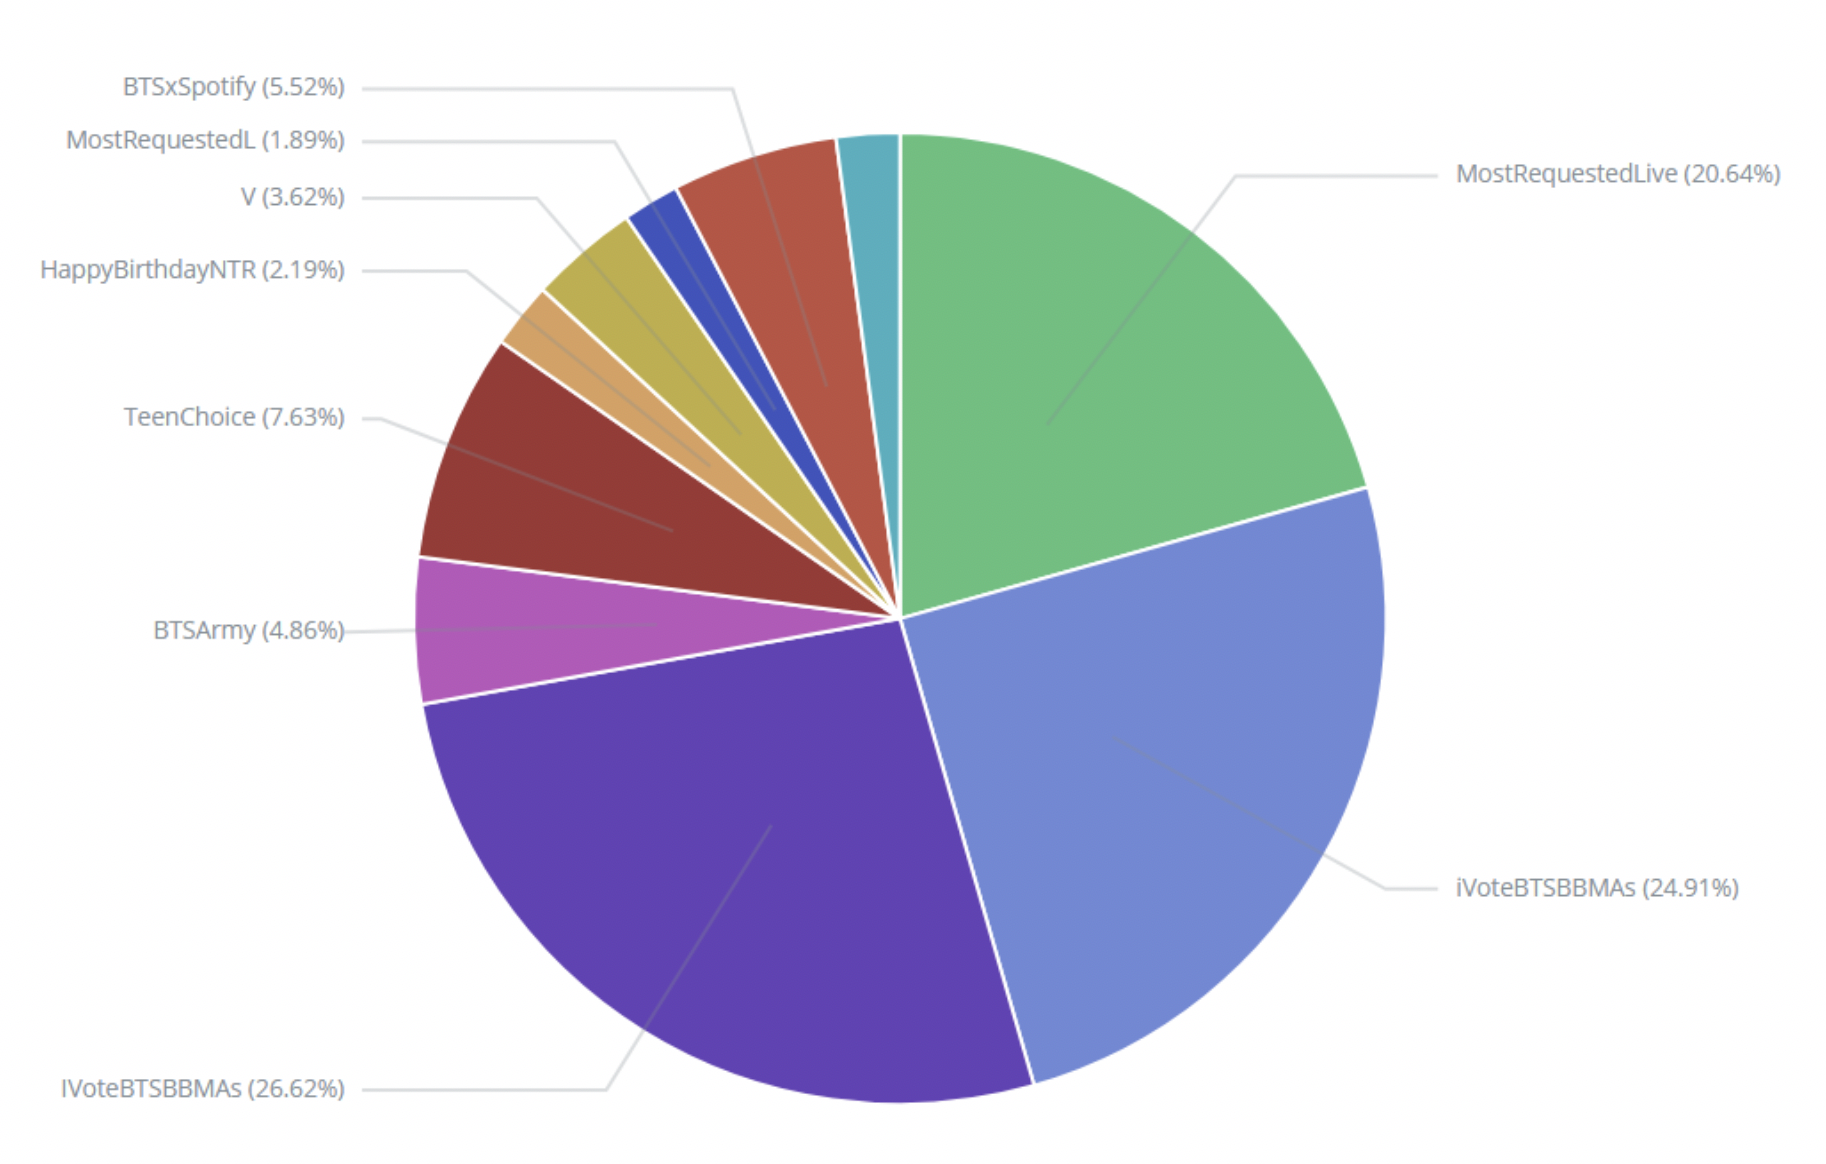
\includegraphics[scale=0.4]{material/architecture/kibana.png}
  \caption{Kibana Analyseplattform} 
  \label{fig:Kibana}
\end{figure}

\section{Fazit}
\subsection{Suchfunktionalität}
Jede moderne Software bietet eine Möglichkeit nach Daten zu suchen. Mit Hilfe von Elasticsearch kann eine einfache Suche nach einer Website oder einem Dokument innerhalb einer Sammlung implementiert werden. Anschließend kann eine Rechtschreibprüfung hinzugefügt werden. Höchstwahrscheinlich ist eine fuzzy Suche und automatische Vervollständigung nötig, möglicherweise sogar während der Eingabe. Da die Relevanz wichtig ist, können fortgeschrittene Ranking-Schemata erstellt werden. Zum Beispiel können Suchergebnisse basierend auf dem Standort, Zeit sowie des Benutzers ausgeführt werden. Und um zu wissen, was die Benutzer tatsächlich tun, kann die Nutzung der Software protokolliert und gespeichert werden für die spätere Analyse der Nutzerdaten.
\newline
Damit ist Elasticsearch eine moderne und mächtige Such-Engine, die fortgeschrittene Suchfunktionalität anbietet und für viele Anwendungsfälle geeignet ist.

\subsection{Performance}
Elasticsearch hat sich als eine robuste und fähige Such-Engine bewiesen, es konnte alle Ziele ohne Einschränkungen erfüllen und zusätzlich mit einer Vervollständigungsfunktion ergänzen. Die Index Konfiguration lässt sich einfach bedienen und über kleine Kalibrierungsschritte im JSON Format von einfachen bist komplexen Indexstrukturen erstellen. Von den Shards, Replicas bis zu den Data-Routings ist Cluster übergreifend alles möglich. Das Suchen ist eine etablierte IT-Disziplin, die mit Komfort, Kosten und Gewinn fest verbunden ist. Demgemäß ist Elasticsearch perfekt geeignet große Datenmengen zu durchsuchen und scheint mit der Anfragegeschwindigkeit, die mit jedem weiteren gefüllten Hardwareknoten die Anfragen automatisch parallelisiert. 
Somit bleibt die Geschwindigkeit im grünen Bereich auch nach dem Anstieg der Datenmenge.  
Allerdings haben die positiv gelisteten Eigenschaften ihre Tücken. Die Konfiguration des Indexes kann im Kleien so wie im Großen geschehen. Die richtige Hardware- (RAM/SSD/HDD) wie Indexkonfiguration muss gewissenhaft gewählt werden, um die versprochenen Geschwindigkeiten zu erreichen. Dementsprechend gewinnt man Zeit durch die automatisierte Datenverwaltung und verliert durch die Elasticsearch Wartung/Feinabstimmung. 

\subsection{Dokumentation und API}
Ebenso problematisch sind die Elasticsearch Abfragen, die einerseits gut im JSON-Format beschrieben und dokumentiert sind, jedoch in der Umsetzung, durch die von Elasticsearch zur Verfügung gestellten JAVA Bibliothek in JAVA schwer verständlich und Komplex in der Umsetzung.
Erst zum Ende des Projekts bin ich auf \textit{Mustach} gestoßen, die \terxtit{JSON-Templats} für die Abfragen erstellt und diese in einer simplen Form an Elasticsearch weiterleitet.  

\subsection{Tools}
Besondere positiv aufgefallen ist die WebUI Kibnan die mit Elasticsearch über REST Anfragen kommuniziert. Es ist möglich nach Daten zu suchen, den Clusterstatus abzufragen sowie aussagekräftige Grafiken zu erstellen. Diese Werkzeuge bieten dem Entwickler einen einfachen und übersichtlichen Einstig in die Elasticsearch-Umgebung. 

	%\chapter{Appendix D}

\section{Section 1}

\end{appendices}

% Esempio
%\index{Esempio |see{Esempio 2}}

\blankpage

%Indice analitico per il momento non verra' messo.
%\printindex %indice analitico


\bibliography{references}
\end{document}

%comandi utilizzati nel template:
%\texttt{} %per scrivere con carattere diverso
%\textbf{} %per scrivere con carattere diverso
%\href{http://www.blob.com/}{testo}
%\index{} %per indice analitico
%\footnote{} %note
%\noindent 
%\label{} 
%\ref{}
%\cite{PdfReference}
%\bibitem{PdfReference}
%®
%
%per inserire una figura:
%\begin{figure}[H]
%\begin{center}
%\includegraphics[width=12cm]{problematiche-del-ciclo-passivo.eps}\\
%\caption{Ciclo attivo e passivo in un'azienda}
%\label{fig:cicliAziendali}
%\end{center}
%\end{figure}
%
%per inserire una tabella:
%\begin{longtable}{p{3cm}p{9cm}}
%\textbf{Titolo} & Descrizione.\\
%\\
%\textbf{Titolo} & Descrizione.\\
%\\
%\end{longtable}
